\lhead{\begin{tikzpicture}[remember picture, overlay]
    \node [anchor=100,inner sep=0] (imagenIZQUIERDA) at (current page header area.north){
\includegraphics[width=18cm]{img/Encabezado.PNG}};
    \end{tikzpicture}}
    \rhead{Ángeles-Hurtado}
    \rfoot{\begin{tikzpicture}[remember picture, overlay]
    \node [anchor=140,inner sep=0] (imagenDERECHA) at (current page footer area.south){
\includegraphics[width=18cm]{img/Foot.PNG}};
    \end{tikzpicture}}
    %----------------------------------------------------------------------------------------
    \lfoot{ \thepage}
    % \renewcommand{\labelenumi}{\alph{enumi}.)} 
    %----------------------------------------------------------------------------------------
    %----------------------------------------------------------------------------------------
    %	TITLE SECTION
    %----------------------------------------------------------------------------------------
    
    \setlength{\droptitle}{-5\baselineskip} % Move the title up
    \title{\textbf{Estudio de tiempos y movimientos en el ensamble de un circuito electrónico utilizando diferentes métodos para su optimización }} % Article title
    
     \author{ 
    \textsc{ Olverpa-Pérez, Eliseo Abraham}\\ 
    %  Afiliación:
    \texttt{ Instituto Tecnológico de Querétaro } \\ 
    \texttt{Tecnológico Nacional de México } \\ 
    \texttt{ Querétaro, México }\\ 
    \texttt{ l22140900@queretaro.tecnm.mx} 
    \and 
    \textsc{Ángeles-Hurtado, Luis Alberto}\\ 
    %  Afiliación:
     \texttt{ Instituto Tecnológico de Querétaro } \\ 
     \texttt{ Tecnológico Nacional de México } \\ 
     \texttt{Querétaro, México}\\ 
     \texttt{alb3rt0.ah@gmail.com} 
    }
    
    
    %----------------------------------------------------------------------------------------
    
    % \begin{document}
    
    % Print the title
    \maketitle
    \thispagestyle{fancy}
    
    %----------------------------------------------------------------------------------------
    %	ARTICLE CONTENTS
    %----------------------------------------------------------------------------------------
    
    % \section*{Resumen}
    % \textit{Palabras clave:}
    % El resumen (ancho de página) deberá contener entre 100 y 200 palabras tipo Adobe Devangari 11 puntos.
    
    \begin{abstract}
    \noindent 
    El resumen (ancho de página) deberá contener entre 100 y 200 palabras tipo Adobe Devangari 11 puntos.
    
    \end{abstract}
    % 
    % 
    \textbf{\textit{Palabras clave}}: Optimización, estudio, movimientos, tiempos, método, circuito.
    % \keywords{First keyword should be the corresponding to the research area according with the authors guide. Maximum of 6 keywords.}
    
    \section{Introducción}
    
    % \begin{itemize}
    %     \item Se debe exponer de manera concreta y en lenguaje sencillo : el tema, o lo(s) objeto (s) de estudio. 
    %     \item Se deben de mencionar las metodologías más usadas muy brevemente. 
    %     \item Se debe de señalar el avance en los últimos años.
    %     \item Al final se debe hacer alusión al o lo(s) objetivos del proyecto de investigación.
    %     \item Debe de tener Referencias científicas, URL, tesis, etc.
    % \end{itemize}
    % Define estudio de tiempos y movimientos
    El estudio de tiempos y movimientos analiza los métodos, materiales, herramientas e instalaciones utilizados en la ejecución de un trabajo. Este análisis tiene como objetivo describir cómo un estudiante promedio de cuarto semestre de ingeniería industrial puede adquirir las habilidades necesarias para desarrollar un proyecto desde cero mediante la implementación de este estudio.\cite{patent}
    Por otro lado el estudio de movimientos tiene por objetivo eliminar o mejorar elementos que afectan a la productividad, seguridad y calidad de la producción. Dando paso a la optimización  El estudio de tiempos es la determinación del tiempo requerido para realizar un proceso, actividad, tarea u operación específica.\cite{parra2020analisis}
     %Ensamble 
     Este estudio estará fundamentado en un ensamble de diversas partes que implementa un circuito electrónico,
     % Circuito electrónico 
     teniendo en cuenta que un circuito electrónico consiste en una estructura de placas formadas por materiales semiconductores, materiales activos y pasivos, cuyo funcionamiento es crear un recorrido completo por el cual pueda viajar la corriente. Depende del flujo de electrones para la generación, transmisión, recepción y almacenamiento de información, con el fin de efectuar una tarea determinada. \cite{thomas2007principios}
    
     Optimización se define como la búsqueda de la mejor manera de realizar una actividad; en este caso, se refiere a optimizar el tiempo de ensamble. Para llevar a cabo este trabajo, se requieren herramientas como el método de tiempos predeterminados, que consiste en una colección de tiempos de movimientos básicos, los cuales se asignan a los movimientos fundamentales y a grupos de movimientos que no es posible evaluar con precisión mediante los procedimientos normales de estudio de tiempos con cronometro. Son resultado del estudio de una muestra grande de diversas operaciones con un dispositivo de tiempos como una cámara de película o de vídeo-grabación capaz de medir elementos muy cortos. \cite{niebel1980ingenieria} \cite{vidalesaplicacion}
     Como objetivo general, el alumno desarrollará habilidades en los campos de la ingeniería de producción, del producto y de la calidad.
    % 
    \section{Justificación}
    
    % \begin{itemize}
    %     \item Se debe de describir lo que se requiere, lo que se necesita o lo que se demanda en la actualidad con un enfoque global pero terminar con menciones a temas locales o nacionales.
    %     \item Debe de tener Referencias científicas, URL, tesis, etc.
    % \end{itemize}
    % 
    % Se debe de describir lo que se requiere, lo que se necesita o lo que se demanda en la actualidad con un enfoque global pero terminar con menciones a temas locales o nacionales.
    % 
    % Cuantos tipos de manufactura existen?
    Desde los años 1800, se han presenciado tres revoluciones industriales que han impulsado significativamente el desarrollo tecnológico. \cite{peemans1992revoluciones}Estas revoluciones han transformado la manufactura, que ha experimentado avances notables y continúa evolucionando en la actualidad. Actualmente, hay diversos tipos de manufactura en constante desarrollo.
    A nivel global, la diversidad y complejidad de la industria manufacturera dificultan la cuantificación precisa del número de empresas dedicadas a esta actividad. Sin embargo, se conoce que México subió de la posición octava a la séptima entre las mayores economías exportadoras de manufacturas del mundo en 2022, desplazando a Taiwán, de acuerdo con datos de la Organización Mundial de Comercio (OMC).\cite{ELECONOMISTA}
    
    Este trabajo permitirá implementar varios métodos como el estudio de tiempos y movimientos para la optimización y mejora del ensamble de un circuito electrónico, ofreciendo un panorama a los procesos y métodos utilizados en la industria para identificar oportunidades y tener un mejor uso de los recursos. 
    % 
    % 
    \section{Descripción del problema}
    
    % \begin{itemize}
    %     \item Se debe describir la desviación o diferencia del ``es'' con respecto al ``debe ser''.
    %     \item Se debe hacer alusión a la incógnita científica*.
    %     \item Debe de tener Referencias científicas, URL, tesis, etc.
    % \end{itemize}
    % \textbf{*La incógnita científica es el elemento cuya solución incrementa el conocimiento científico.}
    % 
    % 
    % ``es''
    Para cada país es fundamental la formación y desarrollo tecnológico ya que representa una competencia a nivel global, que por medio de las diferentes revoluciones industriales se ha permitido el desarrollo de estas competencias tecnológicas, una manera de desarrollar esta competencia es por medio del Estudio del Trabajo buscando generar un mayor rendimiento en la industria, gestionando recursos para su mejor aprovechamiento, entre otras.
    
    En países como México, se observan problemas como la falta de oportunidades laborales para los jóvenes, la insuficiente preparación de los empleados y la informalidad laboral. Los jóvenes enfrentan tasas de desempleo más altas que otras generaciones, generalmente debido a la falta de experiencia laboral.
    
    El estudio del trabajo al ser la encargada de gestionar el uso eficaz de los recursos y establecer estándares, por lo que tendría que permitir a las empresas e instituciones adaptarse a estas transformaciones, mejorando la eficiencia, productividad, lo cual requiere un análisis riguroso con soluciones innovadoras pero la falta de experiencia y conocimientos generan una limitante para la adaptación a las nuevas tecnologías y métodos.
    % 
    \section{Fundamentación teórica}
    
    Es la sección central y de mayor debate, donde debe fundamentarse la hipótesis. Por lo tanto, es esencial señalar claramente la razón y justificación de la suposición, utilizando únicamente referencias científicas. Es crucial retomar el tema presentado en la introducción, pero ahora profundizando para aclarar la incógnita científica y poder plantear la hipótesis. Es necesario abordar la descripción del problema en mayor profundidad, enfocándose en los objetos de estudio. Además, se debe profundizar en las metodologías empleadas para el estudio del tema, utilizando únicamente referencias de artículos y libros científicos.
    
    Plan de Respuesta a Emergencias: Documento técnico que establece la organización y metodología necesarias para la preparación y gestión ante situaciones de emergencia.
    
    Sistema de Tiempos Predeterminados (STP): Conjunto de tiempos para movimientos básicos. Se asignan a movimientos fundamentales y a grupos de movimientos que no pueden ser evaluados con precisión mediante procedimientos normales de estudio de tiempos con cronómetro. Estos tiempos son el resultado del estudio de una gran muestra de diversas operaciones, utilizando dispositivos de tiempo como cámaras de película o vídeo grabación capaces de medir elementos muy cortos.
    
    Therbligs: Son los 17 movimientos en los que se puede descomponer cualquier tarea, mayormente en el ámbito laboral, con el objetivo de determinar la productividad de un operario en su estación de trabajo.
    
    MTM: Significa Medición de Tiempo de Métodos. Es un procedimiento para mejorar métodos y establecer estándares de tiempo, reconociendo, clasificando y describiendo los movimientos necesarios para realizar una operación específica y asignando normas de tiempo predeterminadas a estos movimientos. 
    
    El sistema MTM asigna valores de tiempo para los movimientos fundamentales como alcanzar (inicio del movimiento para tomar algo), mover (desplazamiento con la mano llena), girar (movimiento rotatorio de la mano, muñeca y antebrazo alrededor del eje del antebrazo), asir (tomar o coger con la mano), colocar en posición (ubicación en un sitio específico), desensamblar (separar piezas unidas) y soltar (liberar el control del objeto). 
    
    Los datos de las tablas MTM-1 provienen del análisis cuadro por cuadro de películas cinematográficas tomadas en diversas áreas de trabajo. Estos datos fueron ajustados al tiempo requerido por el operario promedio mediante la técnica Westinghouse.
    
    El formato para el registro de tiempos en MTM se denomina Hoja de análisis de métodos.
    
    El muestreo de trabajo es un método de medición indirecto que, a través de observaciones instantáneas, permite determinar la cantidad de tiempo de actividad o inactividad en un proceso productivo.
    % 
    % 
    % Cuales son las revoluciones industriales que ha vivido la humanidad?
    % A lo largo de la historia del hombre las técnicas manuales para elaborar herramientas y mejorar la caza y la calidad de vida fueron fundamentales para la supervivencia.
    % La revolución industrial han cambiado las fuentes de energía básicas y los medios de comunicación para desplazar mercancías, personas e información.
    % 
    % 
    \section{Hipótesis}
    
    % Es la suposición con fundamento científico relativa a la solución del problema, necesidad o de cómo se aprovecha la oportunidad con la incógnita científica y se fundamenta con: 1. Una suposición (en afirmativo o negativo) y ésta deberá vincularse con:
    % 2. La fundamentación científica que deberá ser precisa 3. Una entidad de comparación para probar la suposición y
    % 4. La variable con que se califica o cuantifica la comparación o se prueba la hipótesis.
    % 
    % 
    El presente proyecto se llevara a cabo con ayuda del estudio de tiempos y movimientos aplicado al ensamble de un circuito electrónico utilizando diferentes métodos del estudio de tiempos y movimientos para su optimización al igual que disminuir el costo del mismo, buscando que el estudiante desarrolle la capacidad para generar proyectos y determinar tiempos estándar. 
    % 
    % 
    \section{Objetivo}
    % 
    % 
    El alumno diseñará, mejorará e integrará sistemas productivos de bienes y servicios aplicando tecnologías para su optimización.
    Diseñará, implementará y mejorará sistemas de trabajo para elevar la productividad.
    En un plazo menor a seis meses y se plasmara en un proyecto integrador.
    % 
    % 
    \subsection{Objetivos específicos}
    % 
    \begin{itemize}
        \item Desarrollar una guía de emergencia para analizar la instalación en la que se llevo acabo la experimentación.
        \item Analizar los métodos, materiales, herramientas e instalación utilizada o que se ha de utilizar en la ejecución del ensamble de un circuito electrónico.
        \item Se establecerá la forma más económica de realizar el trabajo.
        \item Normalizar los métodos, materiales, herramientas e instalaciones.
        \item Determinar exactamente el tiempo necesario para que una persona competente realice el trabajo con una marcha normal.
    \end{itemize}
    % 
    % 
    \section{Metodología}
    
    
    Mediante la metodología de observación y análisis estadístico, se llevó a cabo esta investigación. La recopilación y estudio de datos se efectuaron en la ciudad de Querétaro, en las instalaciones del Instituto Tecnológico de Querétaro (ITQ). Específicamente en el edificio “C”, salón C07, en un horario de 2:00-3:00 pm de lunes a jueves y viernes de 2:00-4:00 p.m. el presente proyecto de desarrollo de febrero a mayo del 2024. 
    
    Se utilizó como caso de estudio el ensamblaje de una tarjeta electrónica, empleando software de diseño asistido por computadora (CAD). En este proceso, se definieron las estructuras a todos los niveles, se establecieron los límites de potencia y control, y se desarrolló la arquitectura requerida para seleccionar la opción más adecuada para su implementación.
    
    En la primera fase de la experimentación, se tomaron dos muestras continuas con una cámara de vídeo. Posteriormente, se aplicaron diversas metodologías para determinar el tiempo de ciclo y el tiempo estándar.
    
    \begin{figure}[H]
        \centering
        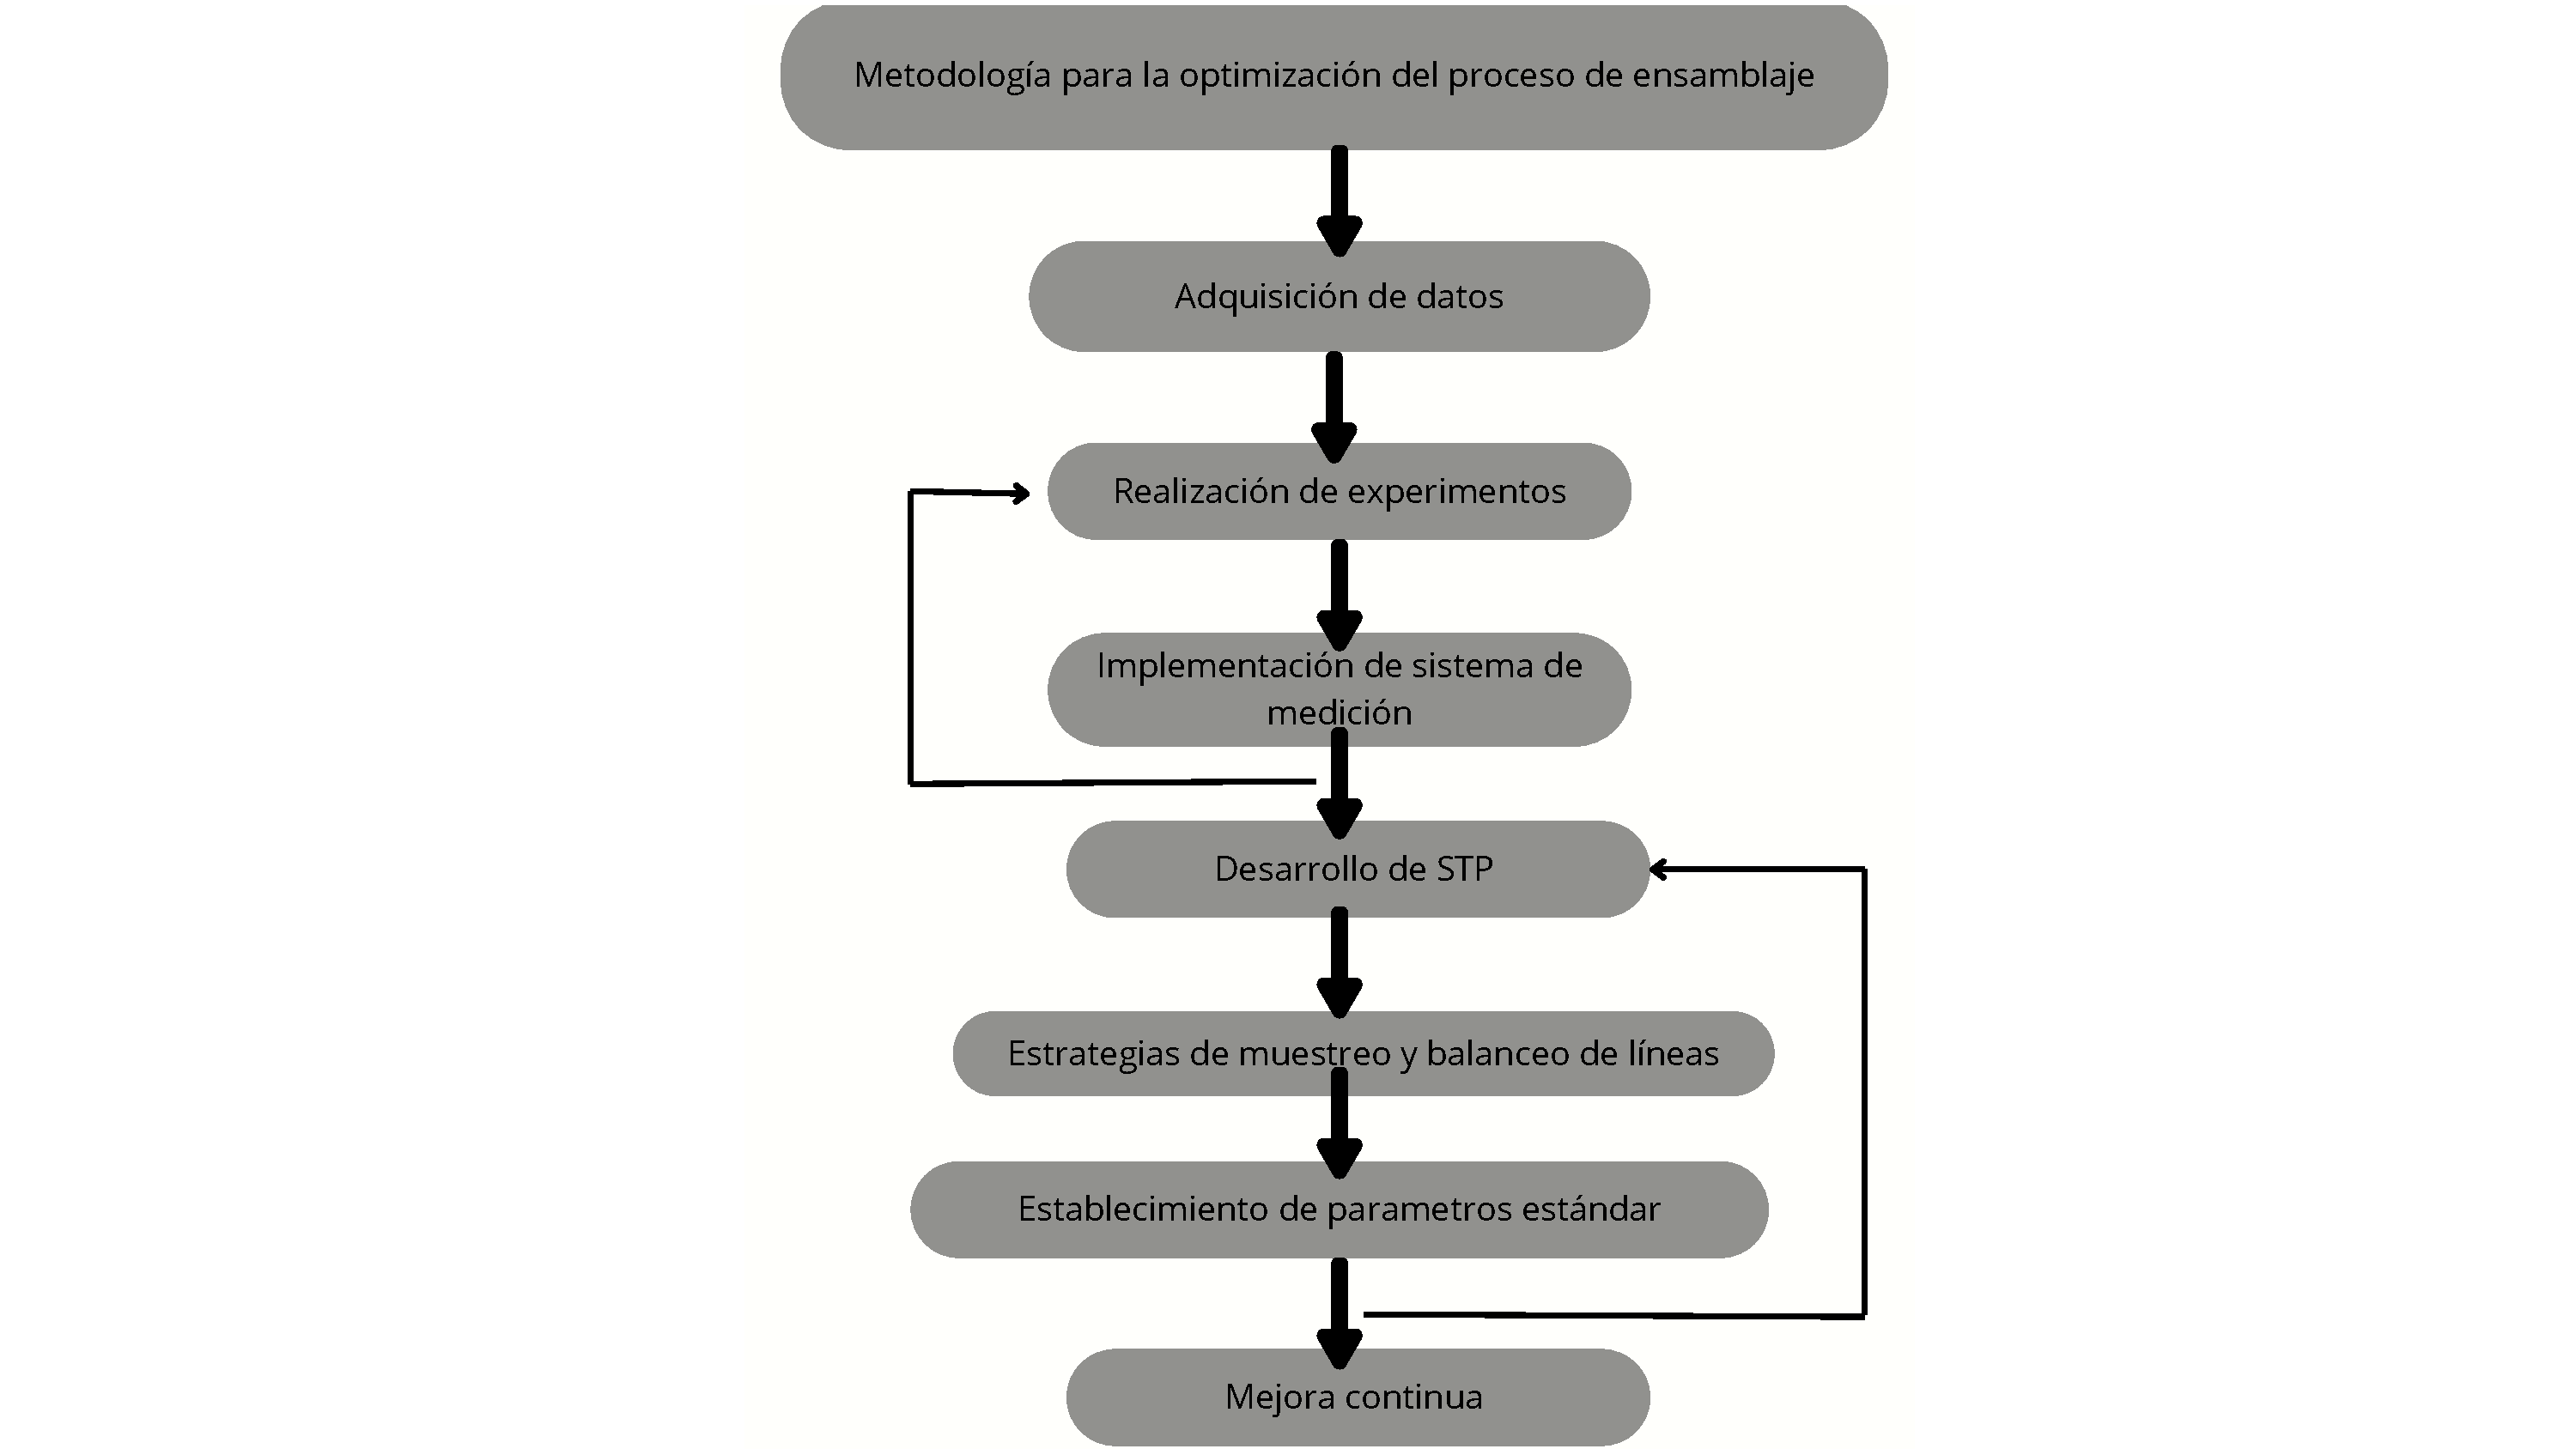
\includegraphics[scale=0.181]{21/img/diagramaMetodología.pdf}
        \caption{Diagrama de la metodología el desarrollo del sistema.}
        \label{fig:diagramaMetodologia}
    \end{figure}
    
    
    \subsection{Desarrollo de la guía de plan de Emergencia}
    
    
    Con esta guía, nuestro objetivo es minimizar las posibles emergencias de incendio y los riesgos de accidentes en el Instituto Tecnológico de Querétaro. Esto se logrará mediante capacitaciones anuales para el personal, las cuales les permitirán tomar decisiones efectivas en situaciones de emergencia para proteger la seguridad de todas las personas dentro y fuera de la institución, así como la integridad de las instalaciones.
    % 
    % 
    \subsection{Análisis de los métodos, materiales, herramientas e instalación utilizada en la ejecución del ensamble de un circuito electrónico}
    
    Se realizo en las instalaciones del Instituto Tecnológico de Querétaro plantel centro, analizando cada factor que se
    
    \subsubsection{Planeación}
    
    Para este proyecto, se propone identificar la forma más eficiente y económica de ejecutar el trabajo. El enfoque estará en detectar áreas de mejora, reducir el tiempo de ciclo y eliminar movimientos innecesarios. Para ello, se recopilarán datos mediante la grabación de un vídeo continuo, lo que permitirá determinar el tiempo con precisión.
    
    Para la ejecución de estas actividades, se empleará una serie de materiales que optimizarán el proceso de ensamblaje. El profesor ha proporcionado la lista de materiales necesarios.
    
    Durante la elaboración de este proyecto, se definió inicialmente el objeto de estudio, que es un circuito eléctrico compuesto por una tarjeta LCD y un ESP-32. En primer lugar, nos familiarizamos con los componentes de este ensamblaje. A continuación, se detallan todos los componentes de nuestro ensamblaje, especificando el modelo y el costo por unidad. Cada uno de los materiales se debe medir, manipular, oler y evaluar para luego representarlos en un programa asistido por computadora, en este caso, se utilizó SolidWorks 2019. Es crucial describirlos en su totalidad.
    \begin{itemize}
    \item El protoboard utilizado en este ensamblaje es una placa para construir prototipos de circuitos electrónicos sin necesidad de soldar. La versión de 300 puntos es más pequeña, ideal para proyectos simples o pruebas rápidas. Tiene 300 puntos de conexión, organizados en filas y columnas con carriles de alimentación en los bordes. Está hecho de plástico ABS con tiras de contactos de cobre o latón recubiertas de níquel.
    \item ESP32-C6: Utilizado para desarrollar aplicaciones IoT, controladores embebidos y proyectos que requieran conectividad inalámbrica. Está fabricado con una placa de circuito impreso (PCB) que incluye un microcontrolador, antena y otros circuitos integrados.
    \item LCD 16x2: Es una pantalla de cristal líquido con 16 columnas y 2 filas de caracteres, generalmente con retro iluminación LED. Su propósito es mostrar información alfanumérica en proyectos electrónicos, como datos de sensores o mensajes del sistema. Los materiales que la componen incluyen vidrio LCD, electrodos de indio y estaño, retro-iluminación LED y una carcasa de plástico.
    
    \item Potenciómetro: Este es un potenciómetro de precisión con una resistencia de 500 ohmios y un diseño robusto. Su propósito es ajustar la resistencia en un circuito, permitiendo el control de variables como el brillo de una pantalla o el volumen de un sonido. Está compuesto por una carcasa de plástico o metal, un elemento resistivo y contactos metálicos.
    
    \item Módulo SPI I2C: Es un adaptador que permite la comunicación entre dispositivos usando los protocolos SPI (Serial Peripheral Interface) e I2C (Inter-Integrated Circuit). Facilita la conexión y comunicación entre microcontroladores y periféricos como sensores, memorias y pantallas. Está compuesto por una PCB con componentes electrónicos como convertidores de nivel lógico y conectores.
    
    \item Regulador de voltaje: Componente que mantiene una salida de voltaje constante independientemente de las variaciones en la entrada o en la carga. Su propósito es proveer una tensión estable a los circuitos electrónicos, protegiéndolos de sobre voltajes y fluctuaciones. El regulador utilizado cuenta con 8 salidas, 3 USB y una tipo C. Está compuesto por semiconductores (transistores, diodos), un encapsulado de plástico o metal y contactos metálicos.
    
    \item Cable USB-C: Este es un cable de conexión con conector USB-C en un extremo, conocido por su reversibilidad y alta velocidad de transferencia de datos. Su propósito es transferir datos y energía entre dispositivos como teléfonos, computadoras y periféricos. Está hecho de conductores de cobre, aislamiento de plástico y conectores metálicos.
    
    \item Resistencias: Son componentes electrónicos que limitan el flujo de corriente en un circuito. Las resistencias utilizadas en este ensamblaje son de 330 ohmios. Su propósito es controlar la corriente y dividir voltajes en circuitos electrónicos. Están hechas de un cuerpo cerámico o de vidrio con una película de carbono o metal, y terminales de alambre de cobre.
    
    \item Cables Dupont-10 Macho-Macho: Conjunto de cables con conectores macho en ambos extremos, de 10 cm de longitud. Utilizados para conectar componentes en protoboards o entre módulos. Utilizaremos 4 de estos en distintos colores. Están compuestos por conductores de cobre, aislamiento de plástico y conectores metálicos.
    
    \item Cables Dupont-10 Hembra-Macho: Conjunto de cables con un conector hembra en un extremo y un conector macho en el otro, de 10 cm de longitud. Sirven para conectar componentes con pines hembra a otros con pines macho, facilitando la interconexión en protoboards y módulos.
    
    \item Almohadilla para soldar:** Superficie resistente al calor utilizada como base para soldar componentes electrónicos. Su función es proteger la mesa de trabajo del calor y proporcionar una superficie adecuada para el proceso de soldadura. También sirve para organizar los elementos del ensamblaje, ya que está dividida en subsecciones de distintos tamaños. Está hecha de silicona o caucho resistente al calor.
    \end{itemize}
    % 
    % 
    \subsubsection{5's}
     
    La implementación de la metodología de las 5S en este proceso de ensamblaje es crucial para mantener nuestro espacio de trabajo organizado, limpio y eficiente. Esto contribuirá a mejorar la eficiencia, la seguridad y la calidad de nuestro producto final. A continuación, se detalla cómo se sugiere aplicar esta metodología en nuestro contexto:
    \begin{itemize}
    
    \item Clasificación (Seiri): Se identificarán y clasificarán todos los componentes y herramientas necesarios para el ensamblaje del circuito eléctrico. Se eliminarán del área de trabajo todos los elementos innecesarios, incluidos componentes defectuosos y herramientas irrelevantes.
    
     \item Orden (Seiton): Los componentes y herramientas se colocarán en lugares designados y etiquetados, facilitando su rápida localización y acceso, y reduciendo el tiempo dedicado a la búsqueda.
    
    \item Limpieza (Seiso): Se realizará una limpieza regular del área de trabajo, asegurando que todo se mantenga en buen estado y funcionando correctamente. Esto incluye la eliminación de polvo, suciedad y residuos que puedan afectar la calidad del ensamblaje.
    
     \item Estandarización (Seiketsu): Se desarrollarán procedimientos estandarizados para la clasificación, organización y limpieza. Se recomienda crear listas de verificación y actualizar el manual de procedimientos con las correcciones pertinentes.
    
     \item Disciplina (Shitsuke): Se capacitará y motivará al personal para que sigan los procedimientos establecidos, y se realizarán supervisiones regulares para asegurar el cumplimiento de los mismos. Esto fomentará una cultura de mejora continua y mantenimiento del orden en el área de trabajo.
    \end{itemize}
    
    
    % 
    \subsubsection{Desarrollo del sistema de tiempos predeterminado}
    Estos 17 movimientos se dividen en dos categorías, efectivos que al ejecutarse implican un avance en el trabajo y los innecesarios que no permiten un progreso en el trabajo, a continuación se mencionaran cuales movimientos pertenecen a que categoría: 
    \begin{itemize}
        \item Efectivos: Alcanzar, mover, tomar, soltar, preposicionar, usar, ensamblar y desensamblar.
        \item Inefectivos: Buscar, seleccionar, posicionar, inspeccionar, planear, retraso inevitable, retraso evitable, descanso y sostener.\cite{IngenieriaIndustrial}
    \end{itemize}
    
    Pero hay que recordar que alcanzar se subdivide en 5 casos
    
    \begin{figure}[H]
        \centering
        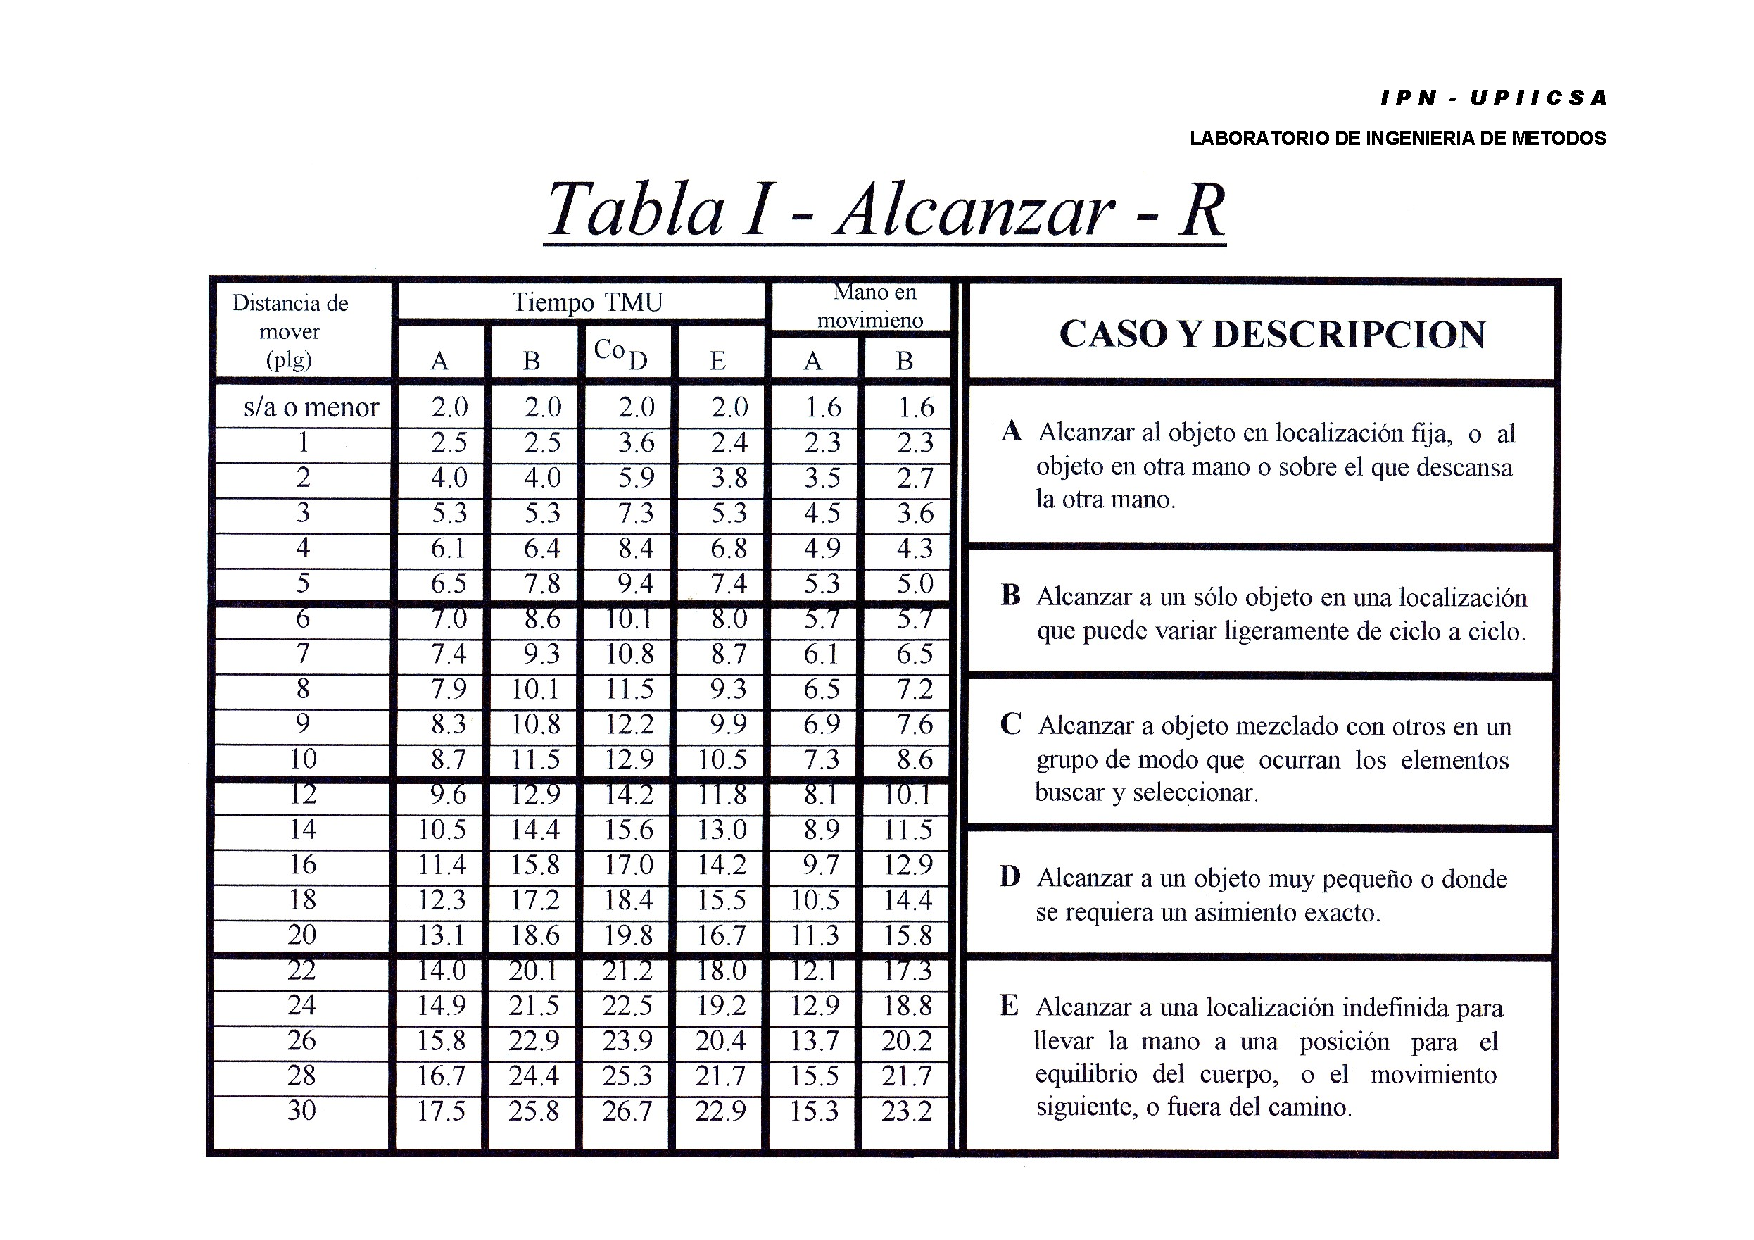
\includegraphics[scale=0.150]{21/img/tabla1AlcanzarR.pdf}
        \caption{Tabla 1 Alcanzar R}
        \label{fig:tabla1AlcanzarR}
    \end{figure}
    
    Y de igual manera la acción de mover se subdivide en 3 casos
    
    \begin{figure}[H]
        \centering
        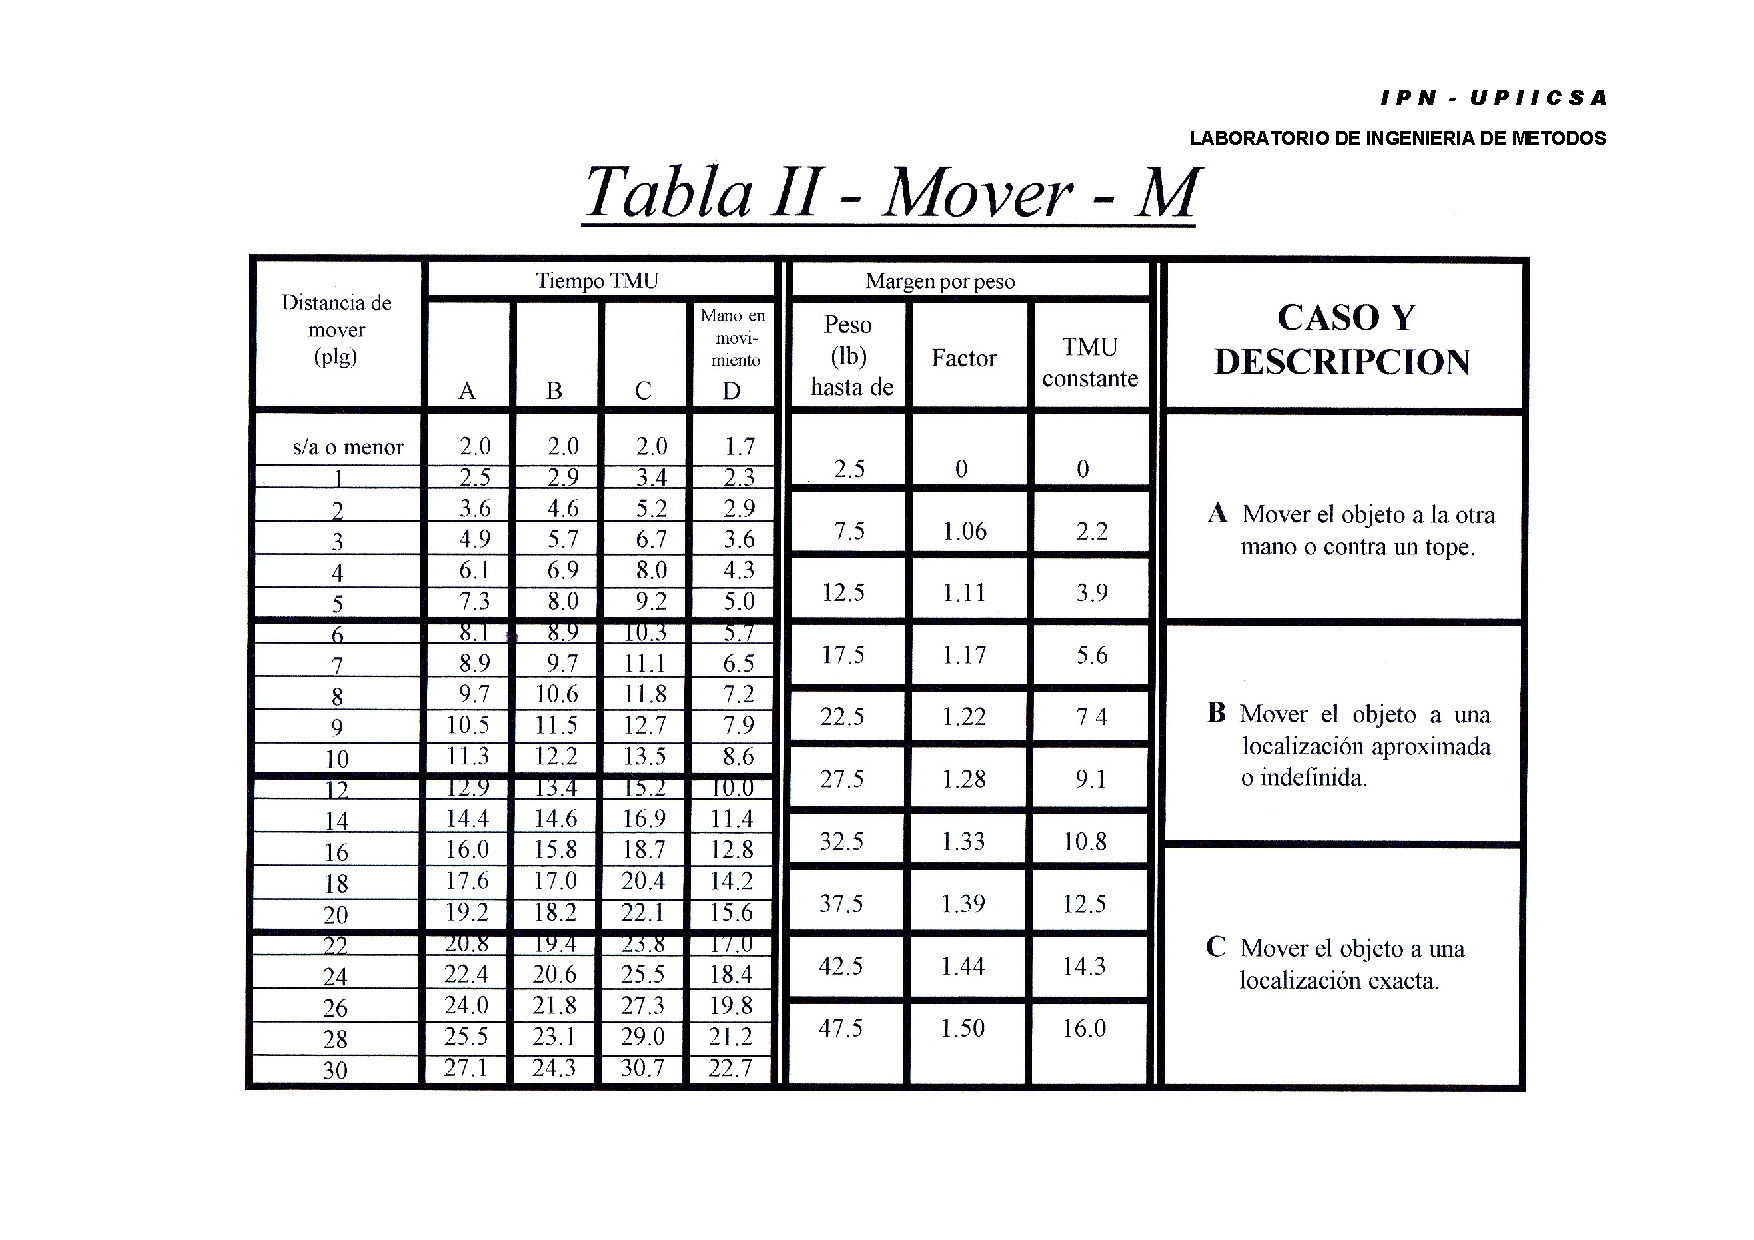
\includegraphics[scale=0.150]{21/img/tabla2MoverM.pdf}
        \caption{Tabla 2 Mover-M}
        \label{fig:tabla2MoverM}
    \end{figure}
    Y los TMU se dividen en las siguientes unidades de medida de tiempo: 
    \begin{figure}[H]
        \centering
        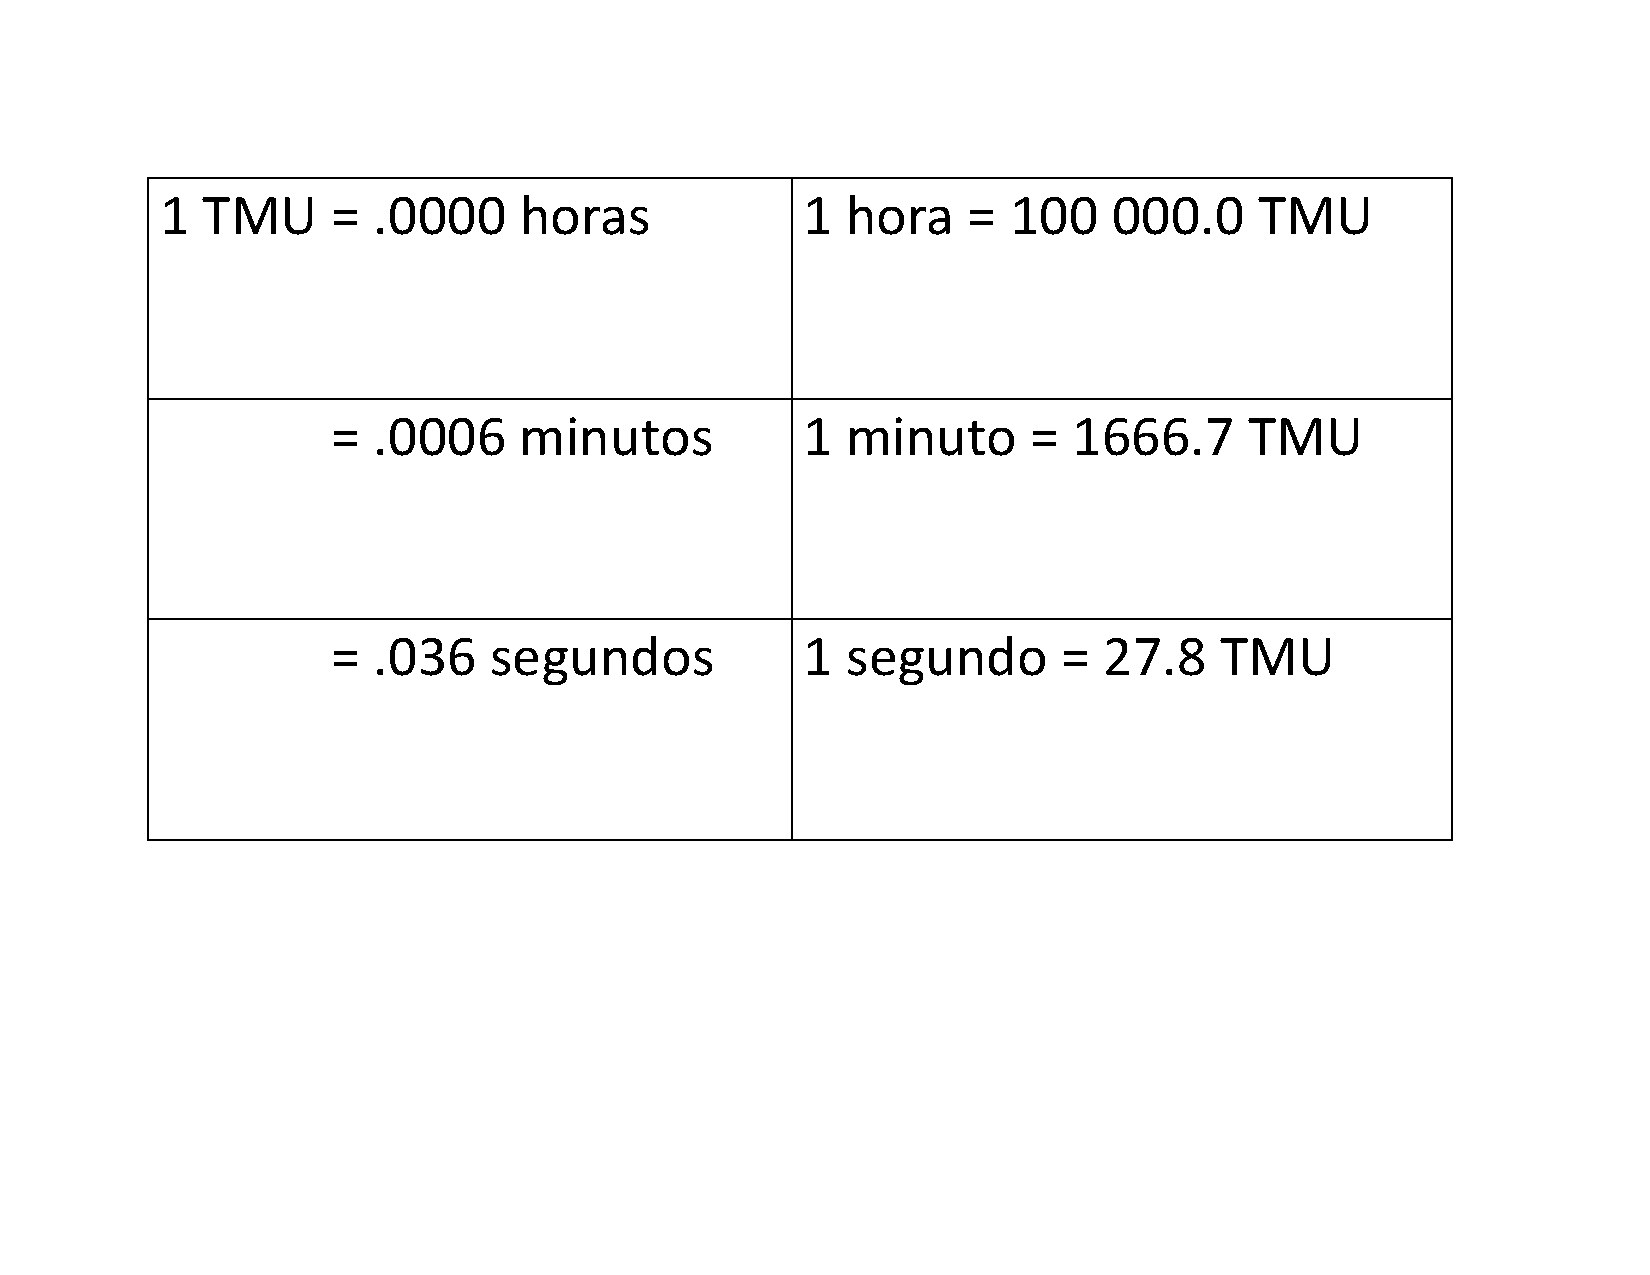
\includegraphics[scale=0.200]{21/img/unidadesMedidaTiempoTMU.pdf}
        \caption{Unidades de Medida de Tiempo (TMU)}
        \label{fig:unidadesMedidaTiempoTMU}
    \end{figure}
    
    
    
    \subsubsection{Desarrollo del muestreo del trabajo}
    
    % 
    \subsubsection{Corrección por balanceo de procesos}
    La corrección por balanceo de procesos es una técnica empleada en la gestión de operaciones y la ingeniería industrial para optimizar la distribución del trabajo a lo largo de una línea de producción o ensamblaje. El objetivo principal del balanceo de procesos es minimizar los tiempos de inactividad y los desequilibrios entre estaciones de trabajo, asegurando que cada estación tenga una carga de trabajo equilibrada y que el flujo de producción sea lo más continuo y eficiente posible. En el proyecto integrador, la aplicación del balanceo de procesos es esencial para mejorar la eficiencia y la productividad.
    % 
    \subsubsection{Datos estándar continuos y discretos}
    Los datos estándar continuos y discretos son dos formas de medir y representar el tiempo empleado en procesos de producción, como el ensamblaje electrónico. Cada tipo de datos estándar tiene características específicas y se utiliza en diferentes contextos .
    \begin{itemize}
    \item Datos Estándar Continuos: Estos datos representan el tiempo en unidades continuas, como minutos o segundos. Se utilizan para medir tareas que fluyen de manera continua y no pueden dividirse fácilmente en partes discretas. Por ejemplo, el tiempo necesario para ensamblar un componente electrónico puede medirse en minutos o segundos.
    
    \item Datos Estándar Discretos: Estos datos representan el tiempo en unidades discretas, como unidades de trabajo o movimientos individuales. Se utilizan para medir tareas que pueden descomponerse en pasos o movimientos separados. Por ejemplo, el tiempo necesario para conectar un cable en un ensamblaje.
    \end{itemize}
    %\begin{figure}[H]
      %  \centering
       % 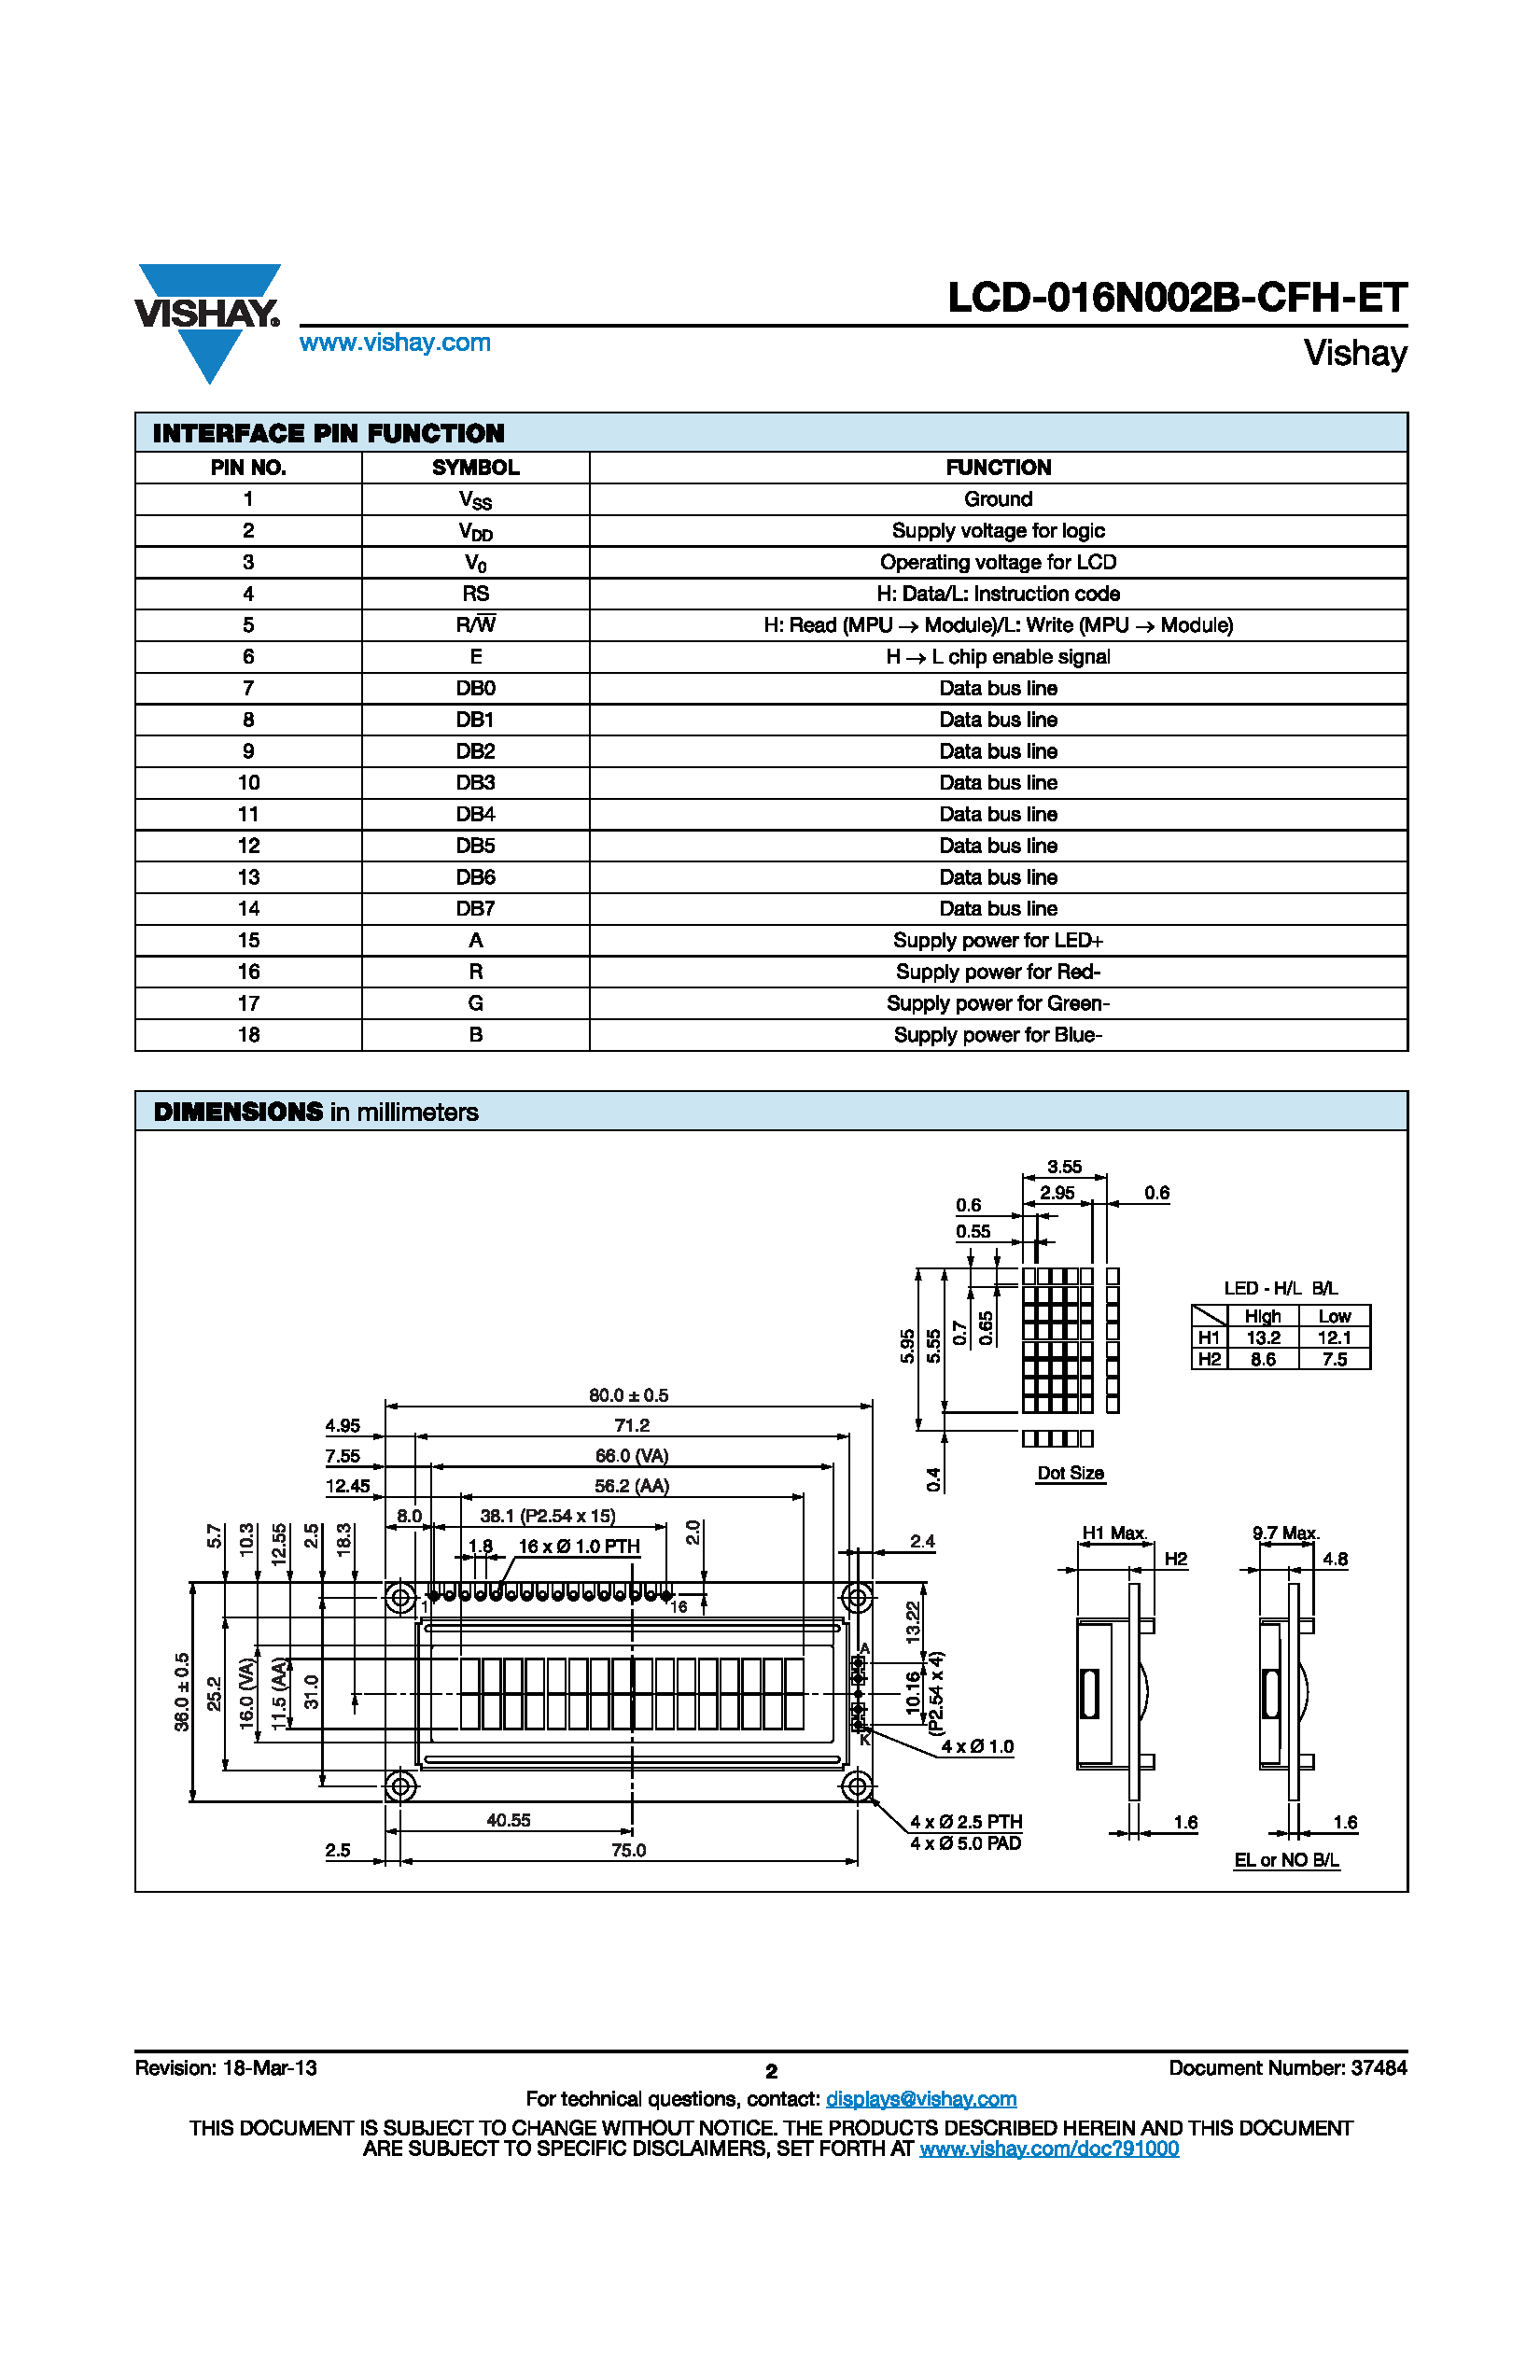
\includegraphics[trim = {30mm 65mm 90mm 250mm},clip,scale=0.5]{6/Img/lcd-16x2.pdf}
        %\caption{Esquema LCD de 16x2}
        %\label{fig:lcd-16x2}
    %\end{figure}
    % 
    % 
    
    % 
    % 
    \subsection{Diseño de la forma más económica de realizar el trabajo}
    
    El diseño de la metodología más costo-efectiva para la ejecución del trabajo se enfoca en identificar la estrategia más eficiente y rentable para llevar a cabo las tareas necesarias en un proyecto o proceso. Esto implica la selección y utilización de métodos, materiales y recursos que minimicen los costos sin comprometer la calidad del producto final. Este diseño es fundamental para maximizar la eficiencia y reducir los costos asociados con el ensamblaje de circuitos electrónicos. Se requiere un análisis exhaustivo de cada fase del proceso de ensamblaje para identificar oportunidades de optimización en términos de costos de materiales y recursos utilizados.
    % 
    % 
    \subsection{Normalización de los métodos, materiales, herramientas e instalaciones}
    
    % 
    % 
    \subsection{Determinación del tiempo estándar para que una persona competente realice el trabajo con marcha normal}
    
    La determinación del tiempo estándar para que una persona competente realice un trabajo con marcha normal implica los siguientes pasos:
    
    1. Selección del trabajo: Elegir la tarea específica que se va a cronometrar.
    2. Registro de tiempos: Observar y registrar el tiempo que varias personas competentes tardan en completar la tarea bajo condiciones normales.
    3. Promedio del tiempo observado: Calcular el tiempo promedio de las observaciones registradas.
    4. **Aplicación de factores de ajuste**: Ajustar el tiempo promedio considerando factores como la fatiga, las pausas y las demoras inevitables para obtener el tiempo normal.
    5. Incorporación del suplemento: Añadir un suplemento por factores adicionales como necesidades personales y demoras inevitables, obteniendo así el tiempo estándar.
    
    El tiempo estándar es el tiempo total que una persona competente necesita para realizar el trabajo con una marcha normal, incluyendo todos los ajustes y suplementos necesarios.
    
     El calculo del tiempo estándar se realiza con la siguiente formula: 
    
     \begin{figure}[H]
        \centering
        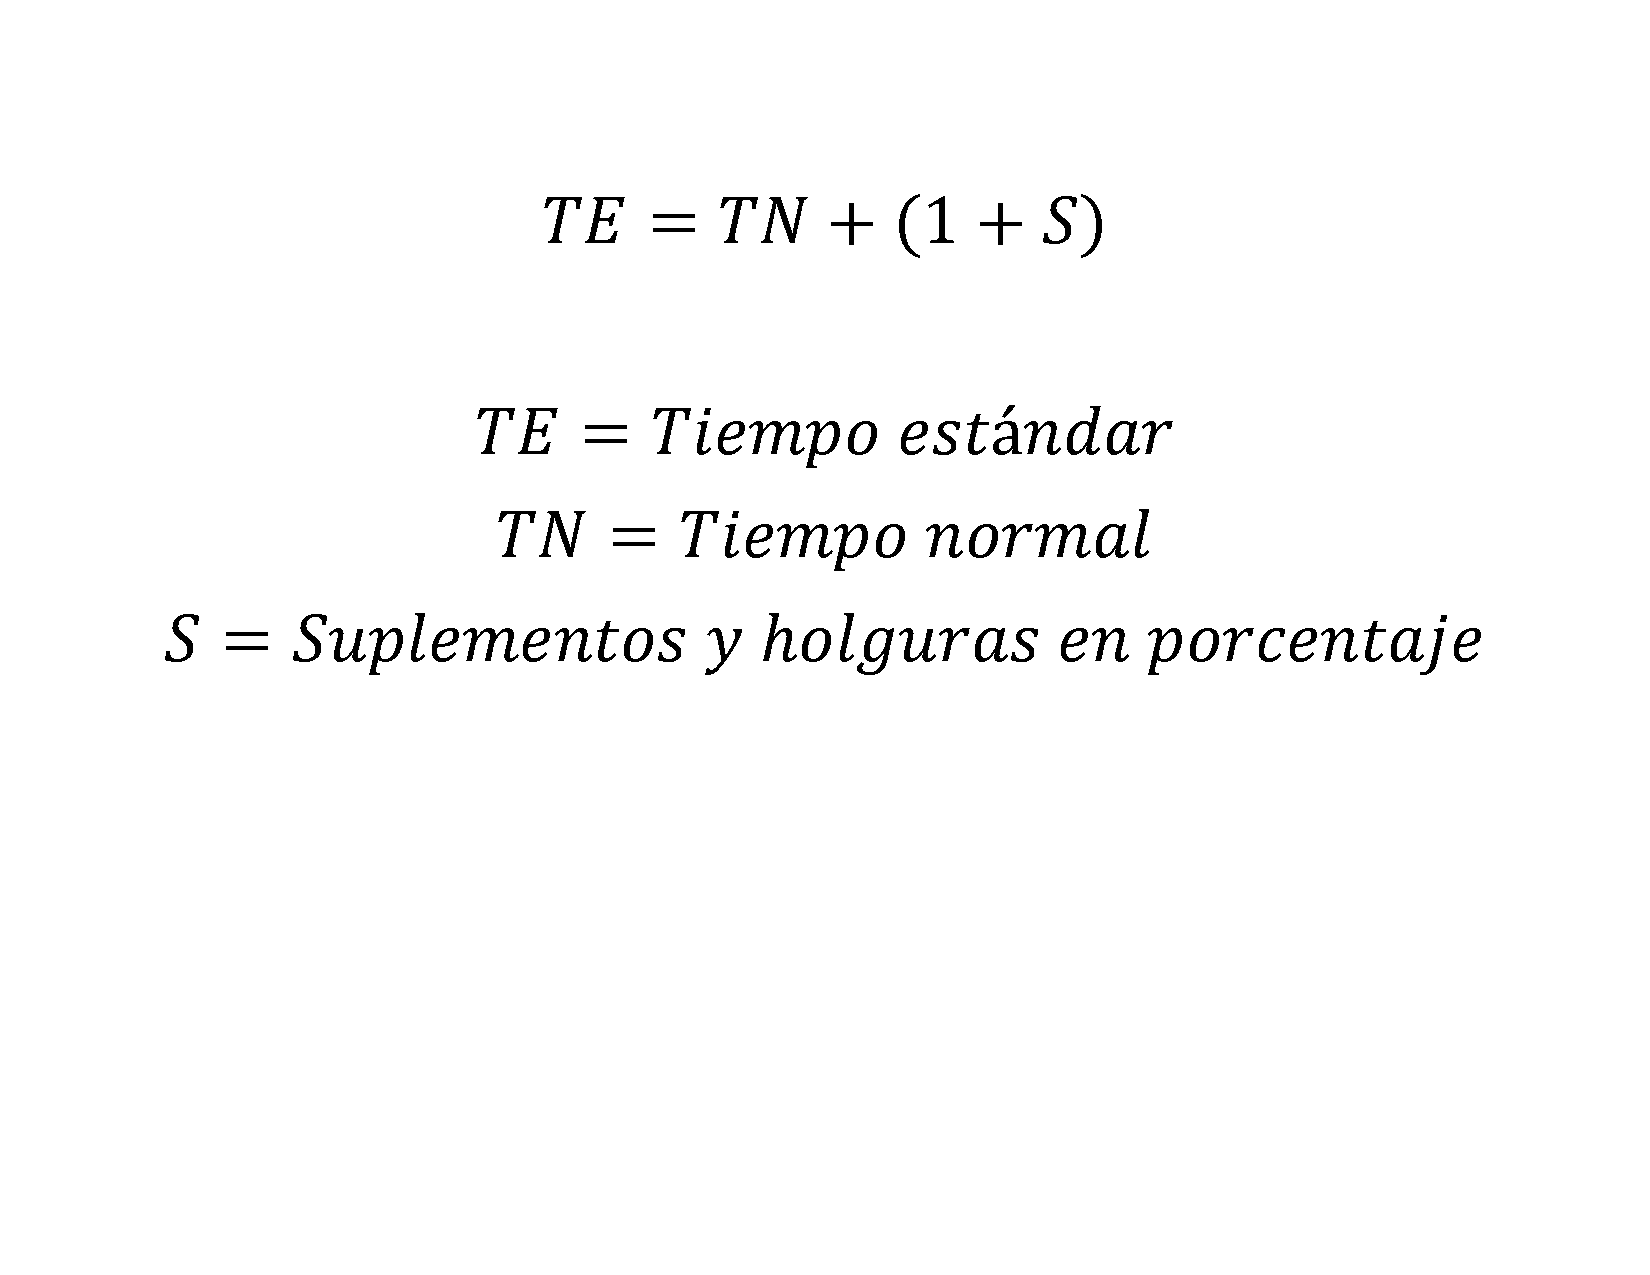
\includegraphics[scale=0.181]{21/img/formulaTiempoEstandar.pdf}
        \caption{Formula Tiempo Estándar.}
        \label{fig:formulaTiempoEstandar}
    \end{figure}
    
    Y las holguras se calculan con la ayuda de las siguientes tablas:
    
    \begin{figure}[H]
        \centering
        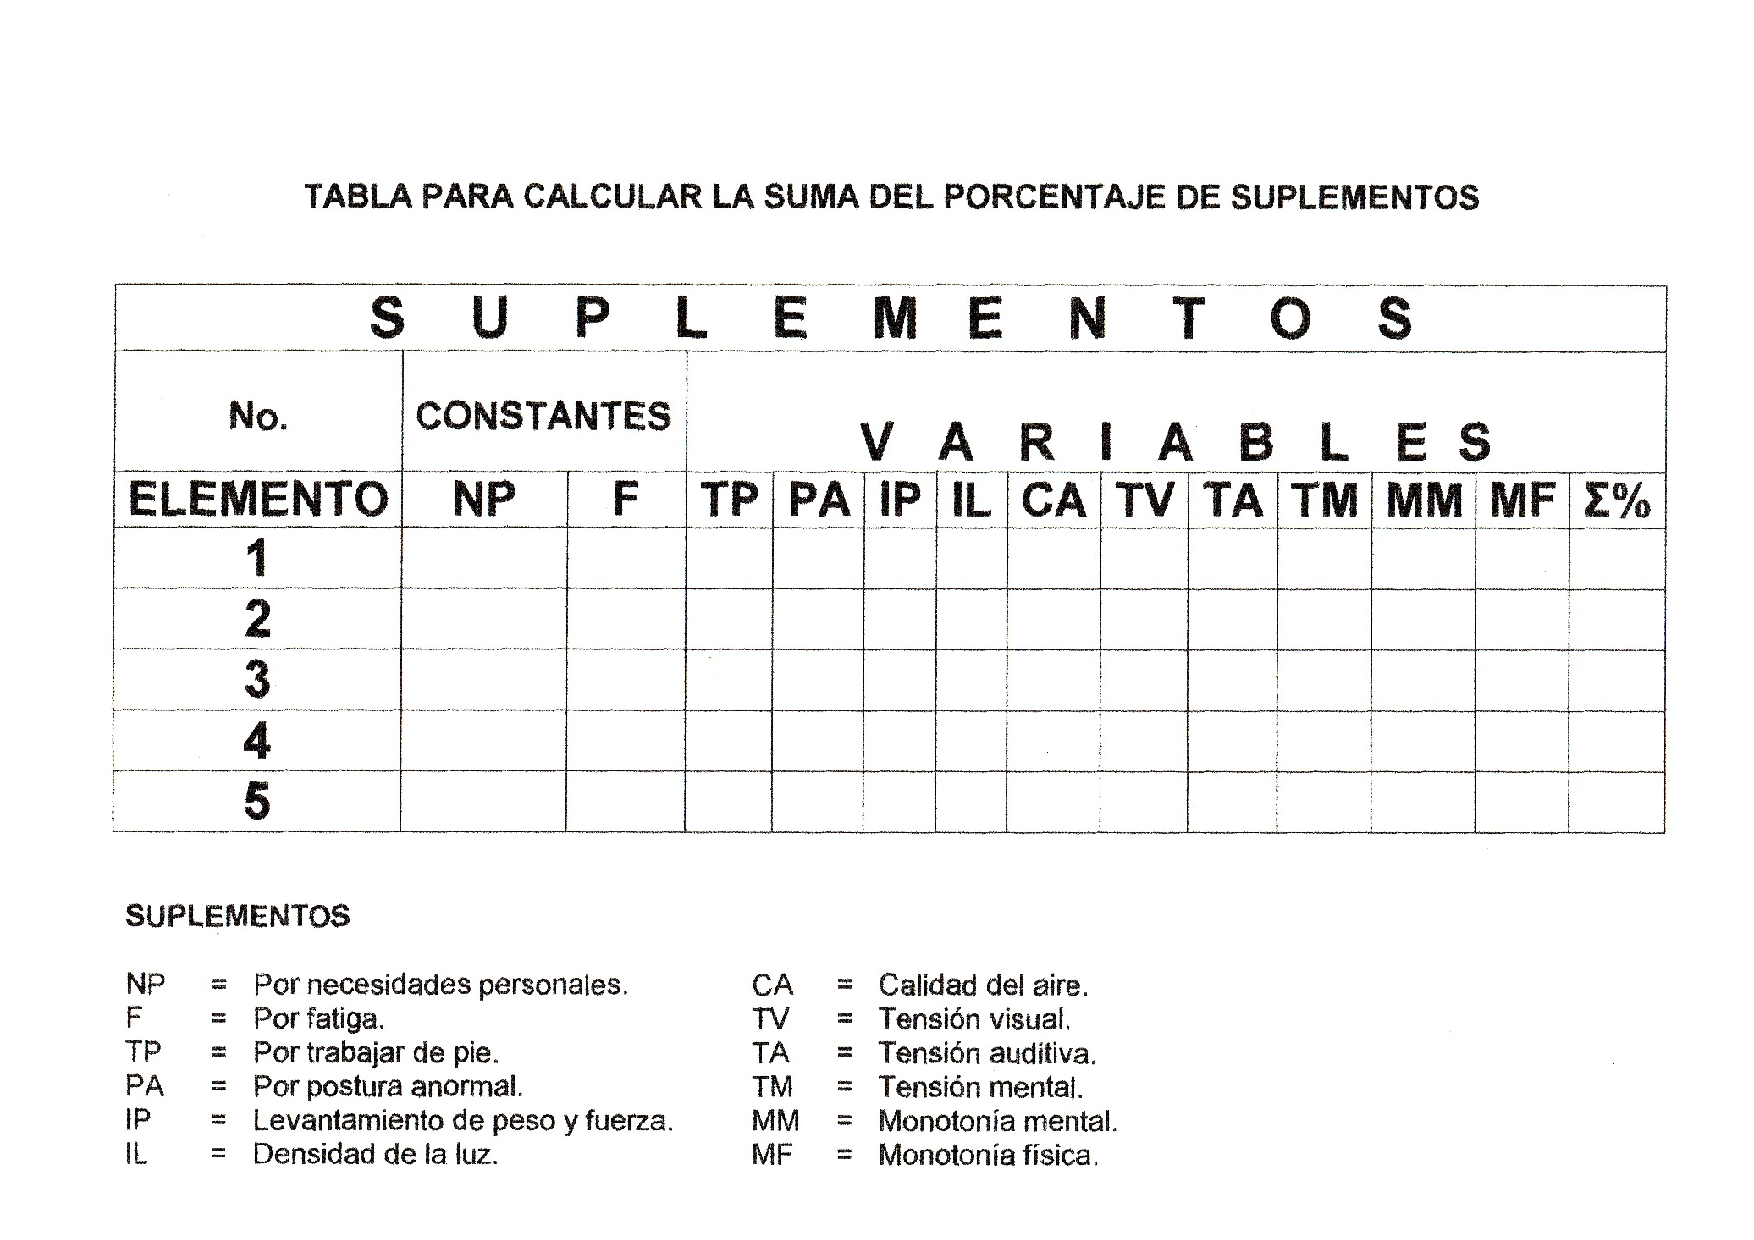
\includegraphics[scale=0.181]{21/img/tablaHolgurasCalculo.pdf}
        \caption{Tabla Calculo Holguras.}
        \label{fig:tablaHolgurasCalculo}
    \end{figure}
    
    \begin{figure}[H]
        \centering
        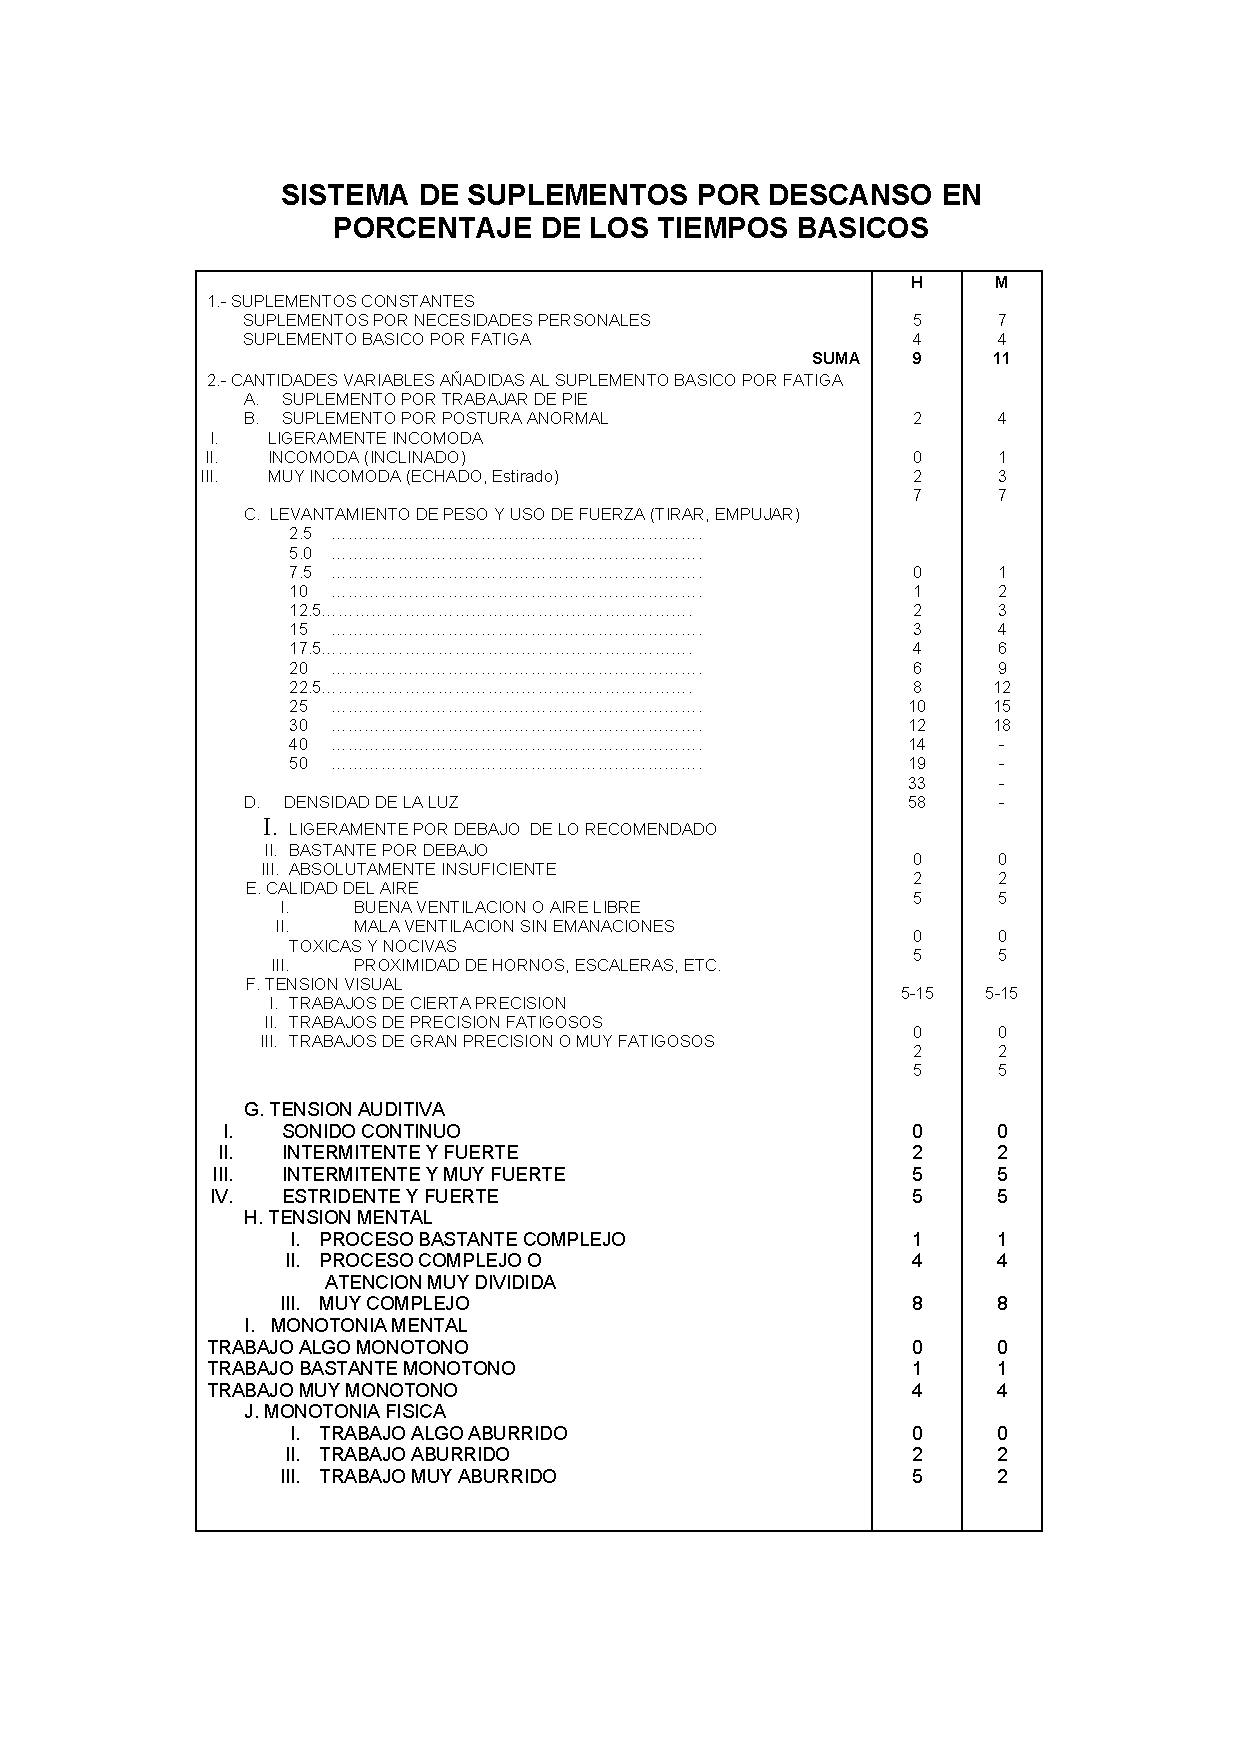
\includegraphics[scale=0.181]{21/img/tablaHolguras.pdf}
        \caption{Tabla Holguras}
        \label{fig:tablaHolguras}
    \end{figure}
    % 
    % \subsection{Acrónimos y Abreviaciones}
    
    % Los acrónimos y abreviaciones deberán ser definidos únicamente la primera vez que aparecen en el texto, esto para que el lector entienda lo que significan.
    
    % \subsection{Ecuaciones}
    
    % Las ecuaciones son una excepción a las especificaciones prescritas de esta plantilla. 
    % Deberá determinar si su ecuación debe escribirse o no utilizando la fuente Adobe Devangari. 
    % Para crear ecuaciones multinivel, puede ser necesario tratar la ecuación como un gráfico e insertarla en el texto después de aplicar el estilo de la platilla.
    % Las ecuaciones serán enumeradas de manera consecutiva, y el número de ecuación, entre paréntesis, se colocan al ras de la derecha, utilizando una tabulación derecha.
    % 
    % \begin{equation}
    %     \label{eq1}
    %     x + y = z 
    % \end{equation}
    % 
    % Es importante asegurarse de que los símbolos de la ecuación sean definidos antes o inmediatamente después de la ecuación. Utilice “(1)”, en vez de “Eq. 1” al enumerar las ecuaciones, excepto al principio de una oración: “La ecuación (\ref{eq1}) es…”
    
    \section{Resultados y discusión}
    
    \subsection{Desarrollo de la guía de plan de Emergencia}
    
    Con esta guía buscamos disminuir en su totalidad las emergencias de riesgo de incendio, así como el riesgo de accidentes en el Instituto Tecnológico de Querétaro \ref{fig:mapaUbicacion} identificando al personal que cuente con capacitación de por lo menos una vez al año para que en caso de emergencia se tome la mejor decisión para salvaguardar la integridad física de clientes internos y externos, así como de las instalaciones
    Evaluando cada riesgo interno por un rango para dar prioridad en las acciones véase Tabla %\ref{tab:nivelesRiesgos}..
    
    %\begin{figure}[H]
     %   \centering
     %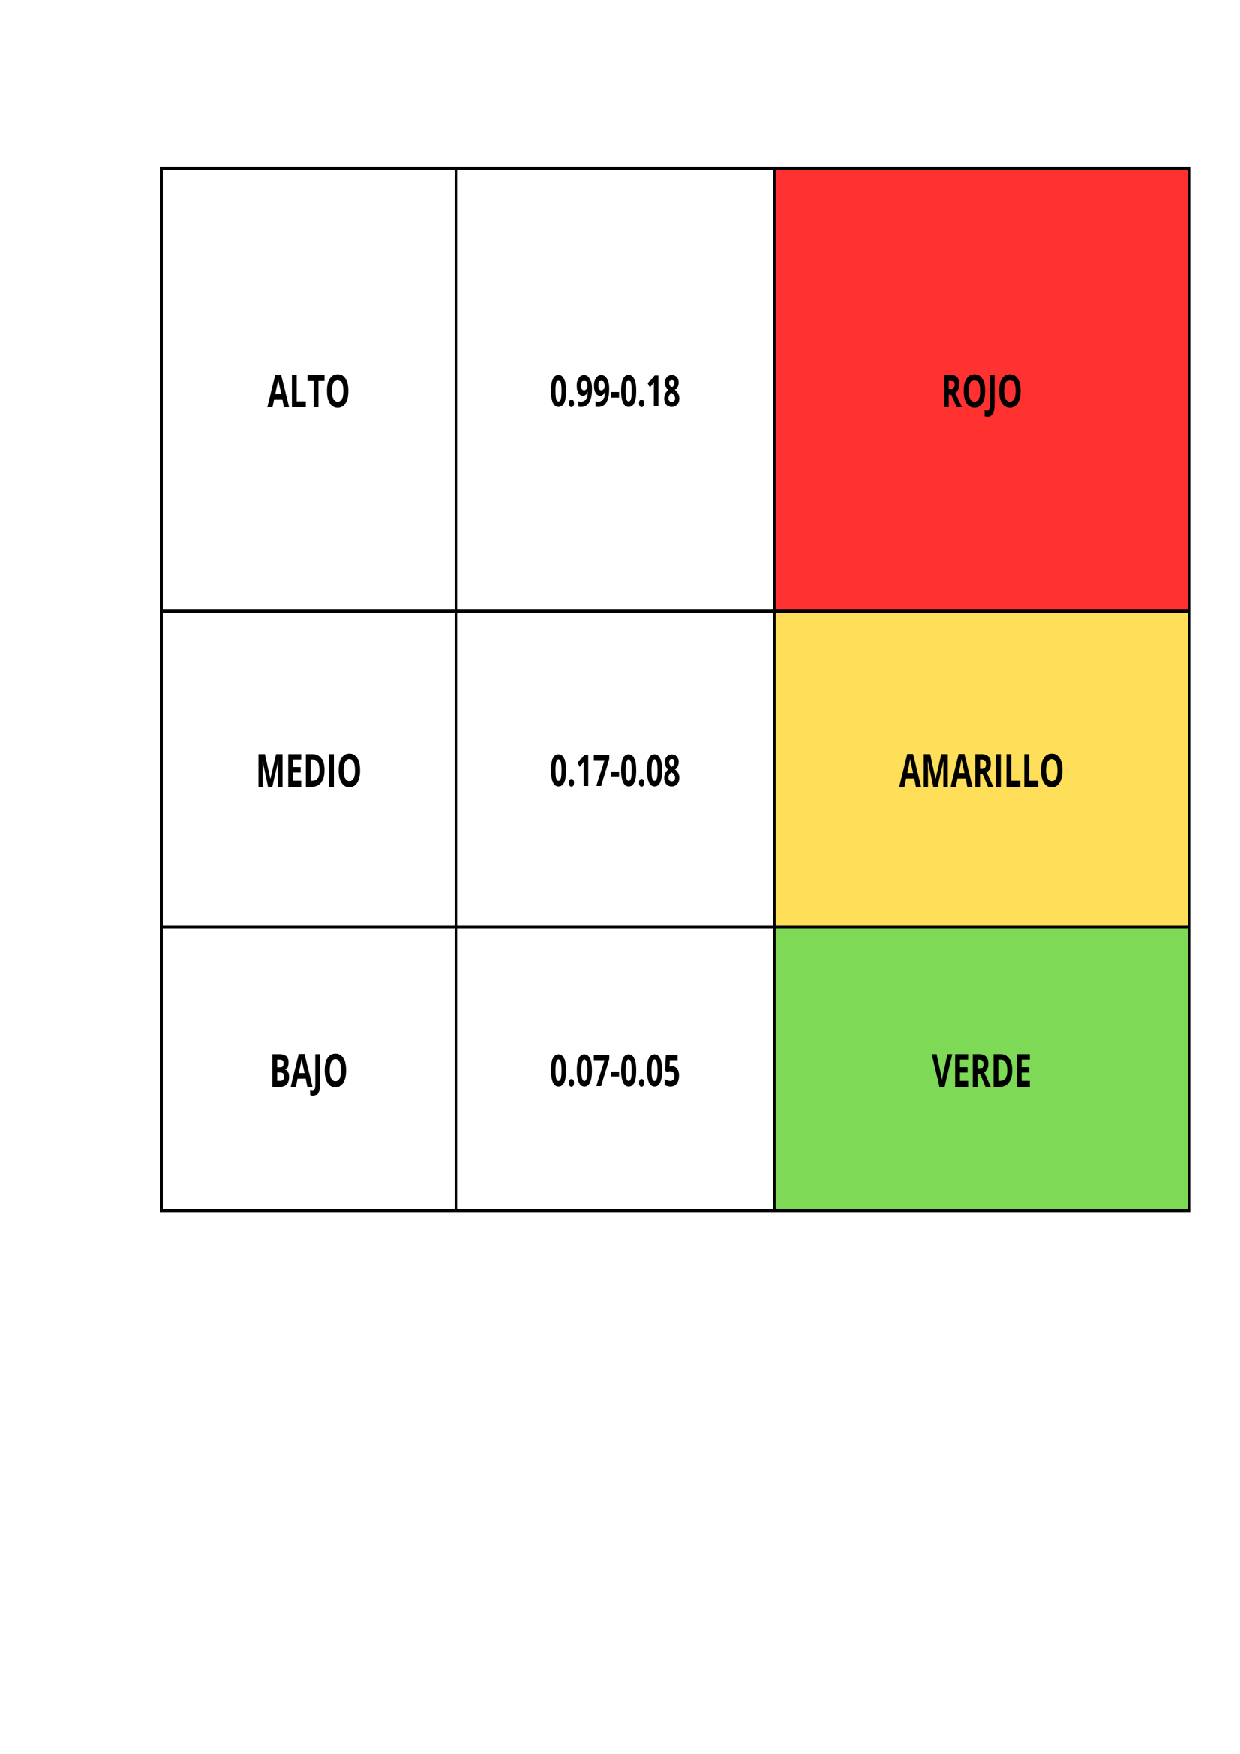
\includegraphics[scale=0.150]{21/img/nivelesRiesgos.pdf}
      %  \caption{Niveles de Riesgo}
       % \label{fig:nivelesRiesgos}
    %\end{figure}
    
    \begin{figure}[H]
        \centering
        \includegraphics[scale=0.150]{21/img/mapaUbicacion.pdf}
        \caption{Tecnológico Nacional de México, Instituto Tecnológico de Querétaro, Av. Tecnológico S/N, Centro Histórico, Centro, 76000, Querétaro, Qro., 4422274400 Ext. 4423}
        \label{fig:mapaUbicacion}
    \end{figure}
    
    % 
    \subsubsection{Identificación del riesgo}
    
    Estamos comprometidos a mantener todos los días un programa interno de prevención de riesgos, así como una retroalimentación por parte de clientes internos y externos en los riesgos que se presentan en las actividades constantes por su parte invitamos a utilizar el equipo de trabajo \ref{fig:matriz}.
    
    \begin{figure}[H]
        \centering
        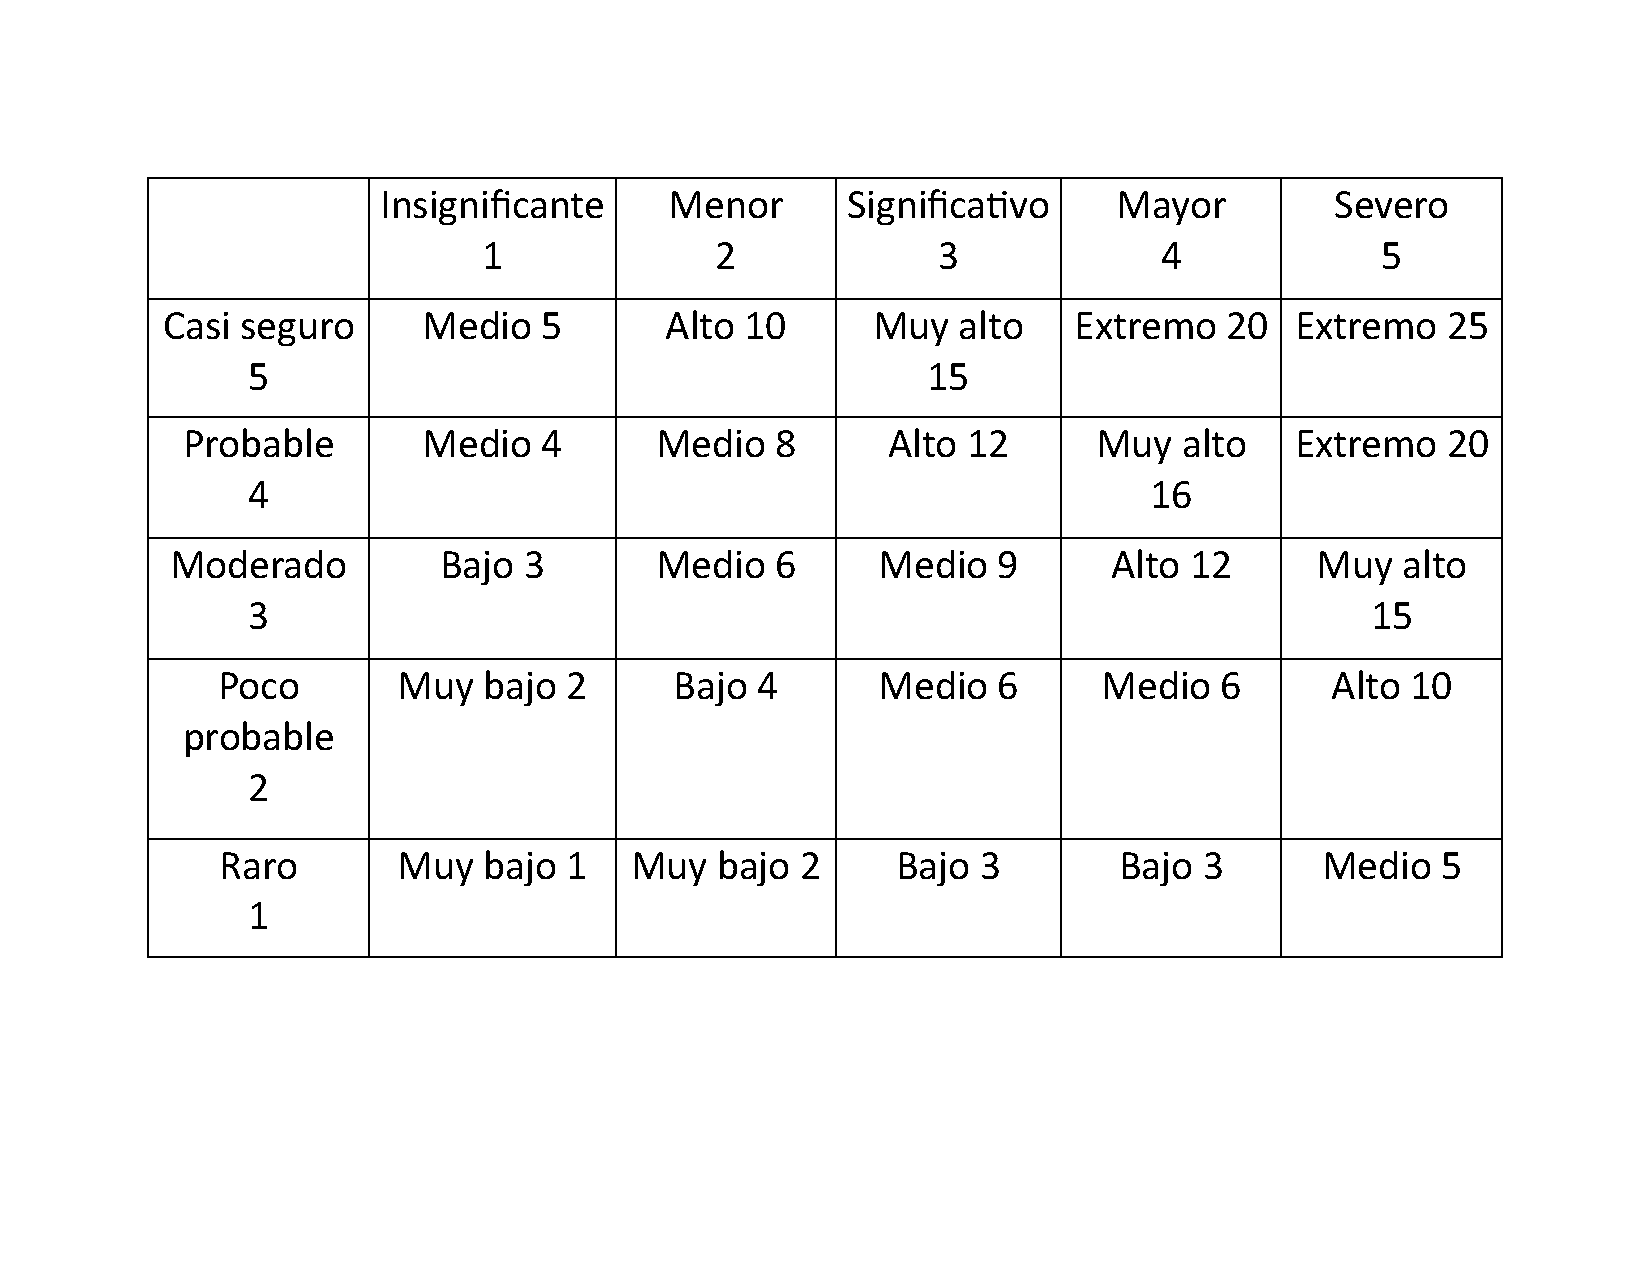
\includegraphics[scale=0.28]{21/img/matriz.pdf}
        \caption{Matriz de riesgos}
        \label{fig:matriz}
    \end{figure}
    
    % 
    \subsubsection{Riesgos internos}
    
    El riesgo se define como la posibilidad de que algo suceda o no suceda en otras palabras es la proximidad de un daño, el siguiente diagrama definirá la determinación de dichos riesgos, véase Figura \ref{fig:diagramaIdentificacionRiesgos}. 
    
    \begin{figure}[H]
        \centering
        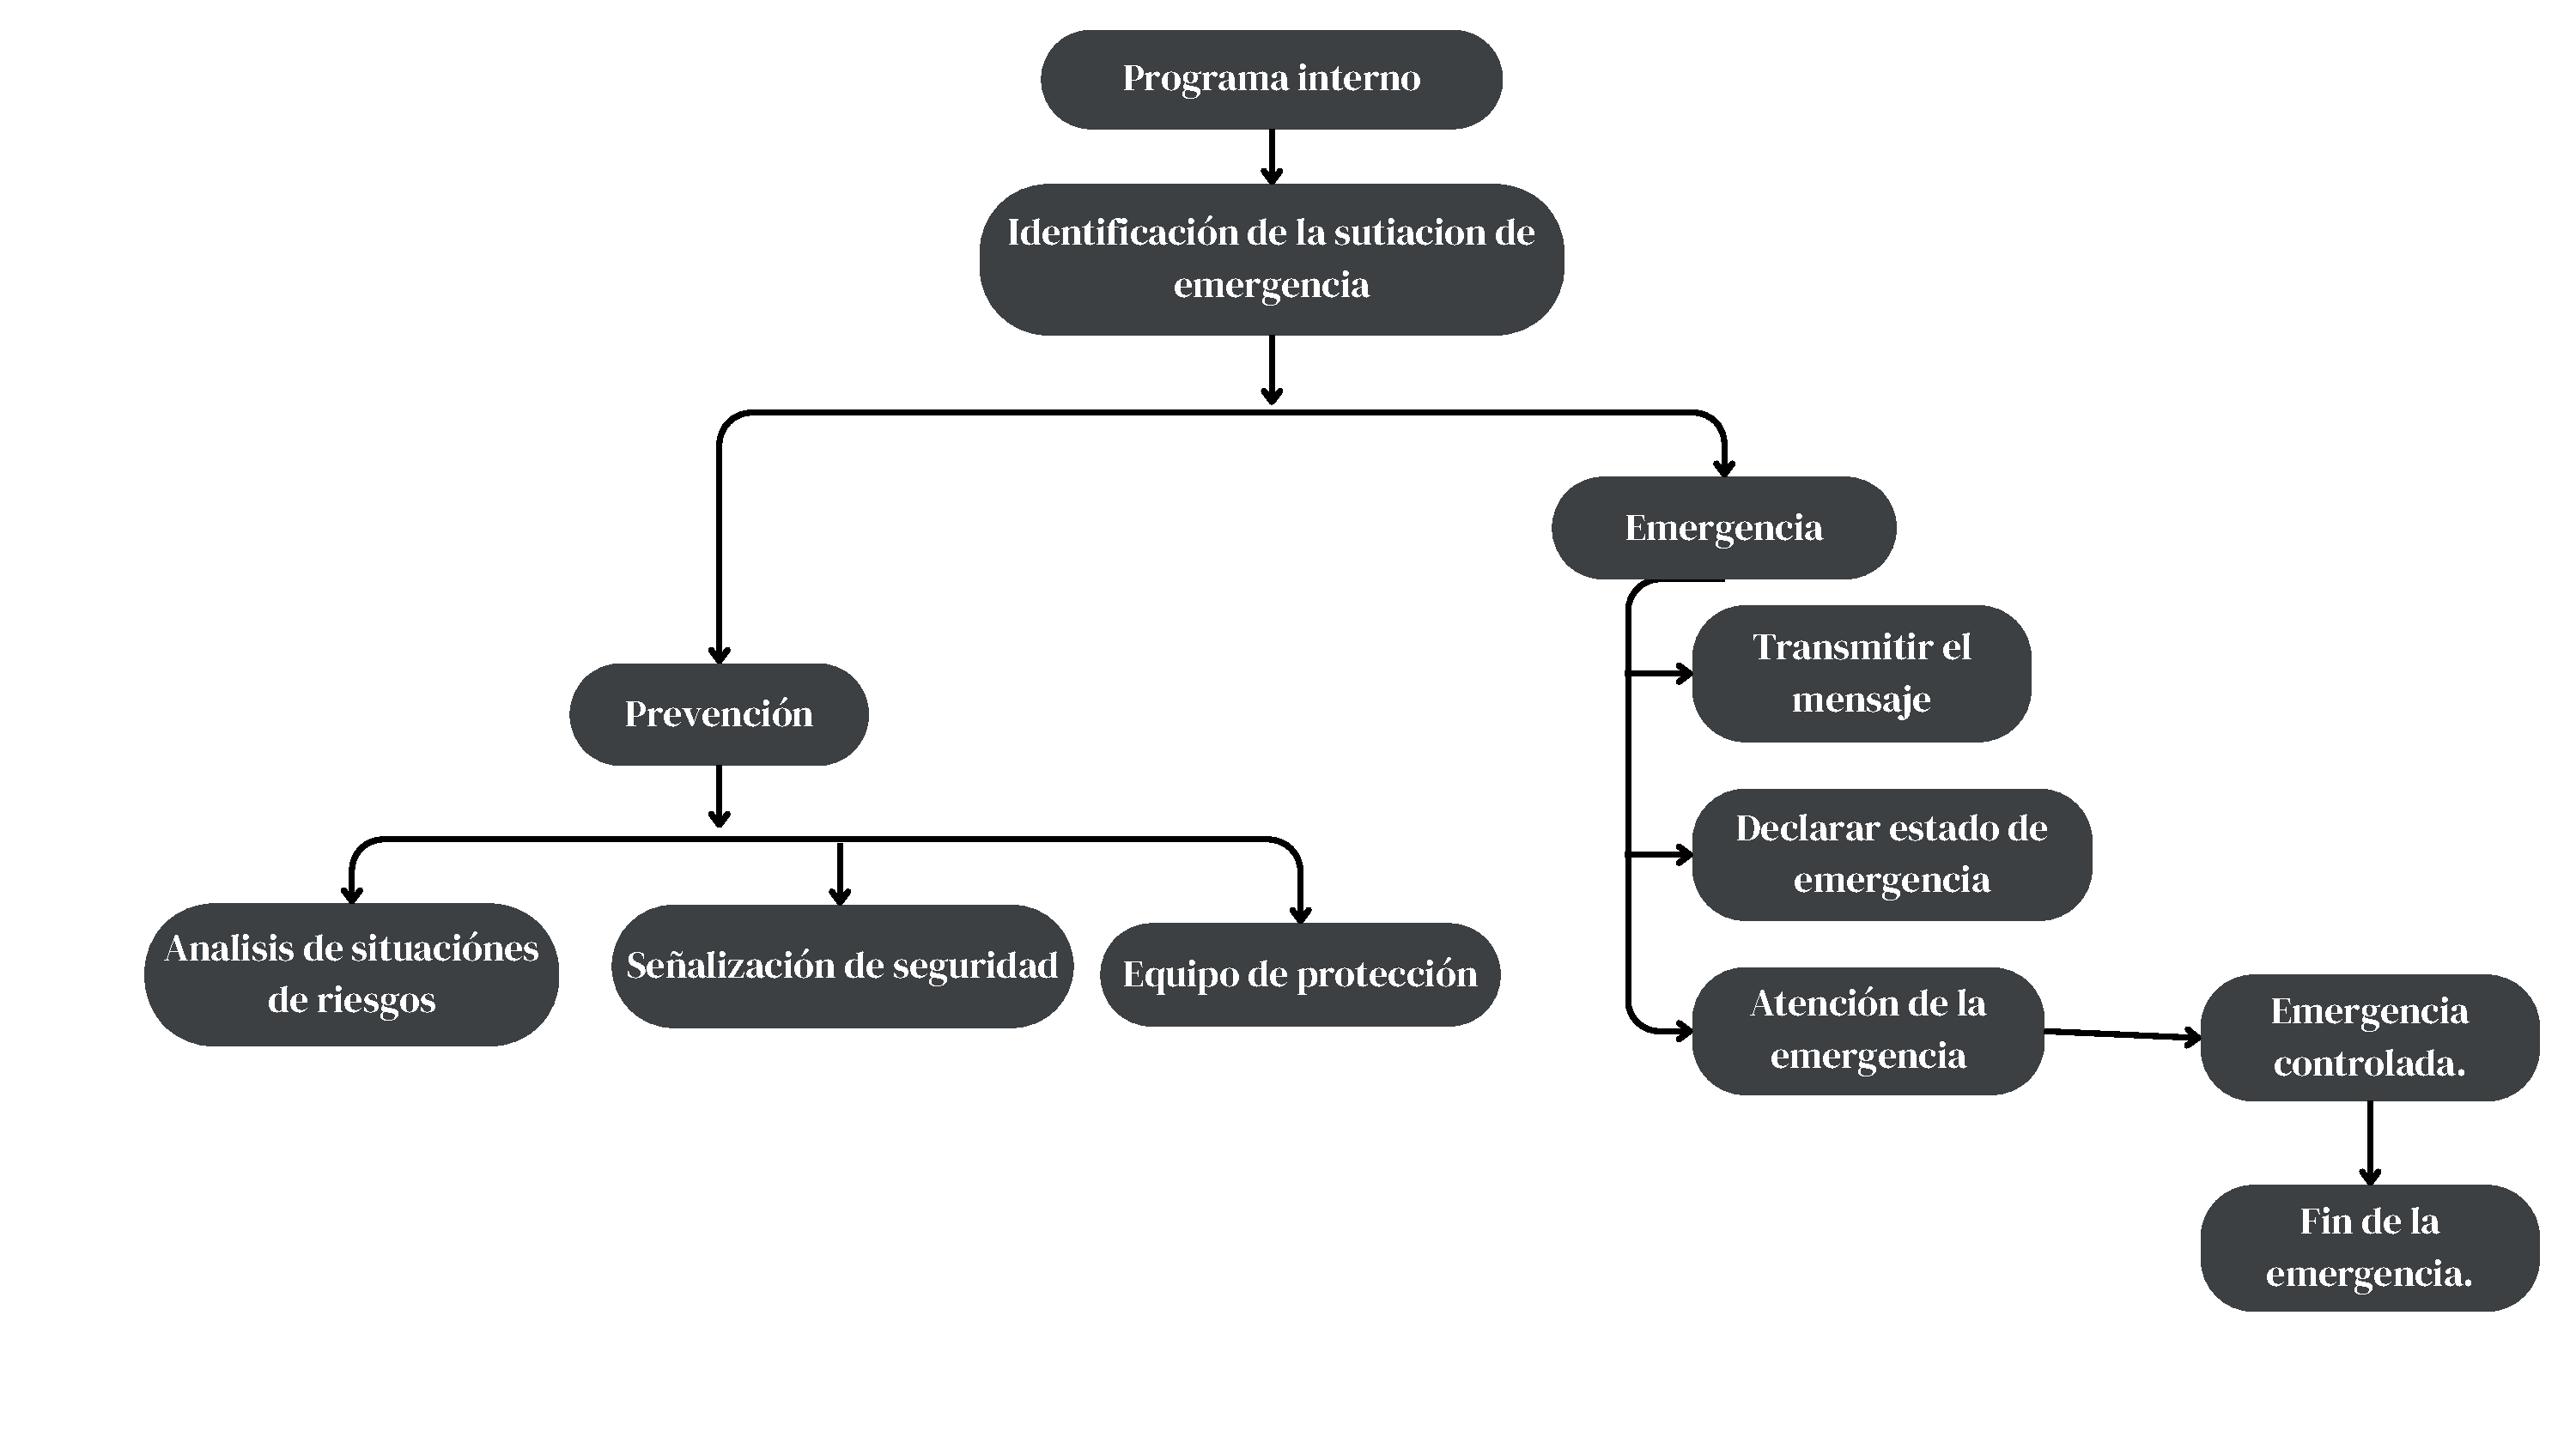
\includegraphics[scale=0.150]{21/img/diagramaIdentificacionRiesgos.pdf}
        \caption{Diagrama de identificación de riesgos}
        \label{fig:diagramaIdentificacionRiesgos}
    \end{figure}
    
    El riesgo operativo interno lo definimos como la posibilidad de que sufre la empresa derivado de los fallos naturales en su propio funcionamiento, mostrándose en la siguiente tabla \ref{fig:riesgosInternos} los riesgos internos que se determinaron en base a el diagrama anteriormente mostrado.
    % 
    \begin{figure}[H]
        \centering
        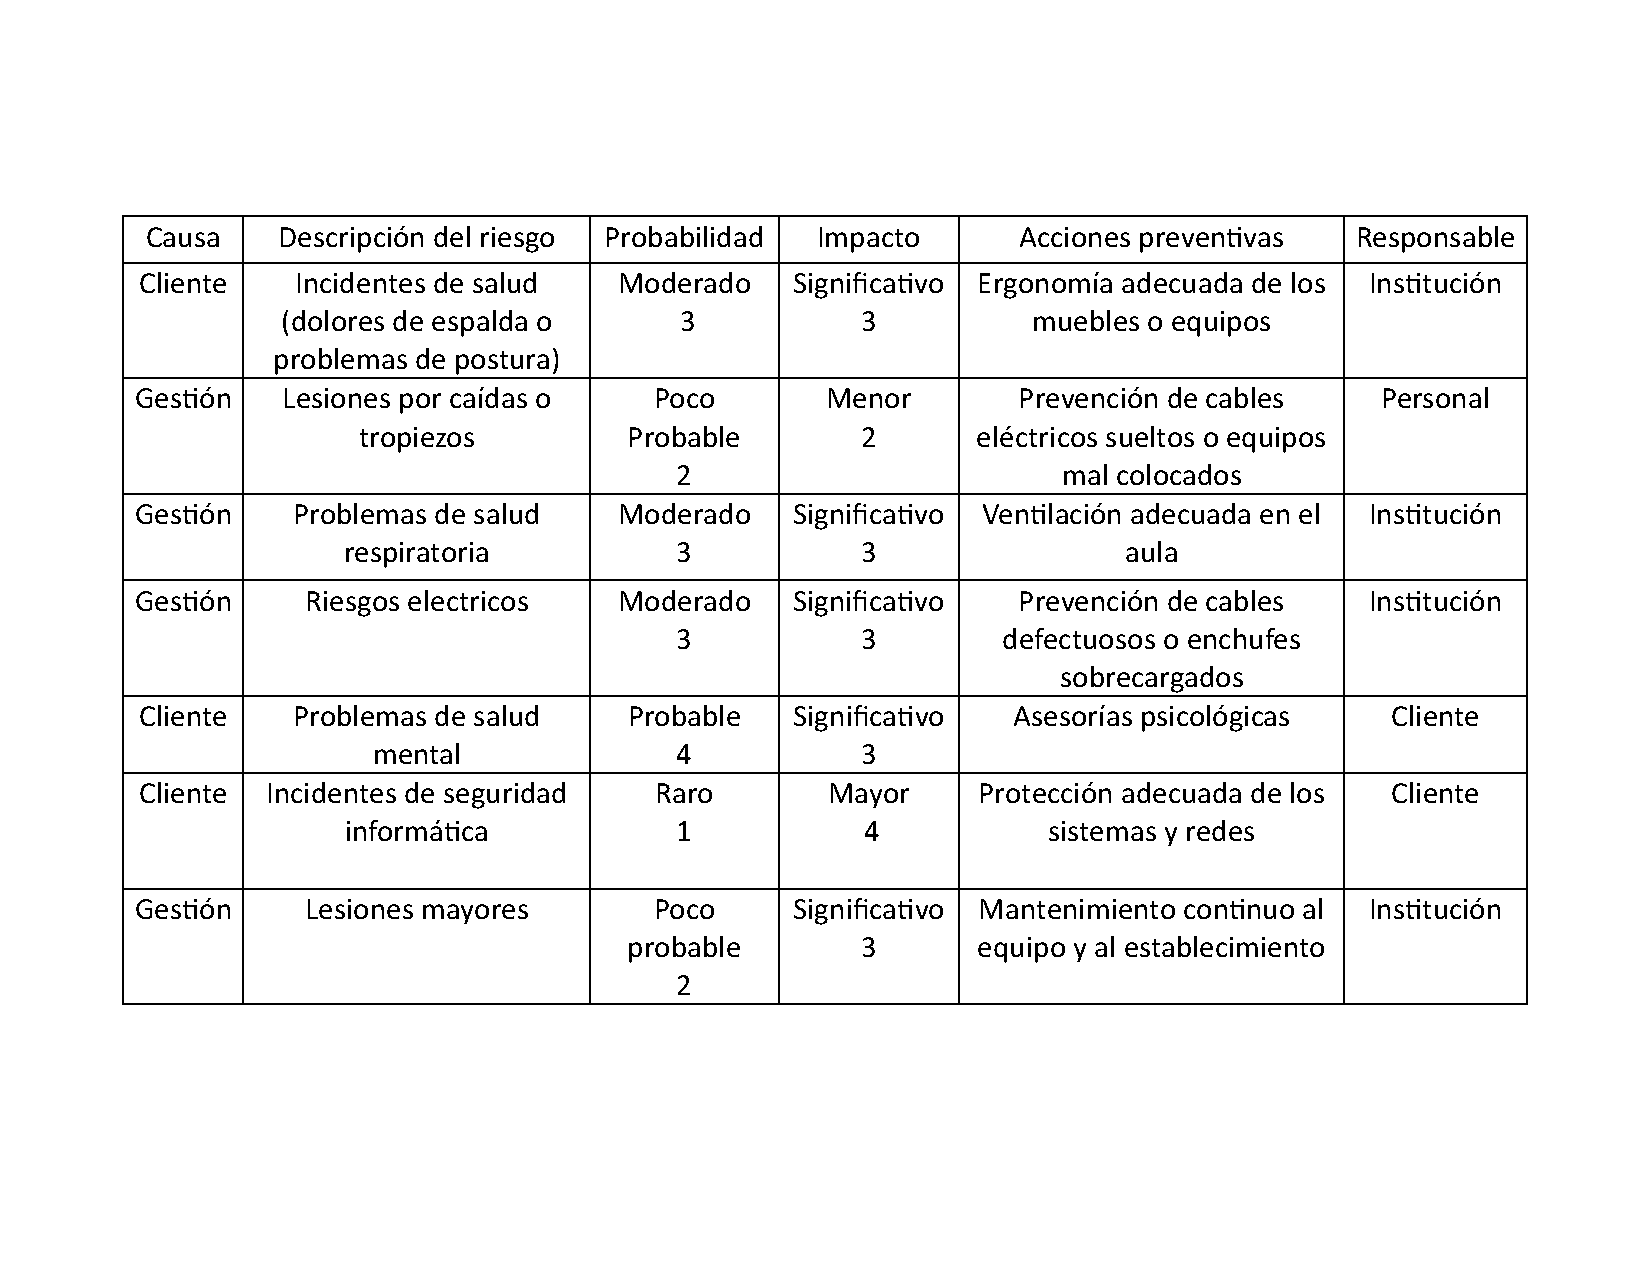
\includegraphics[scale=0.3]{21/img/tablaRiesgosInternos.pdf}
        \caption{Riesgos Internos}
        \label{fig:riesgosInternos}
    \end{figure}
    
    
    
    % 
    \subsubsection{Riesgos externos}
    
    Descripción de los riesgos externos.
    % 
    % 
    \subsubsection{Programa de actividades de prevención y auxilio}
    
    Declarando las diferentes acciones de lo que se piensa hacer cuando ocurra un riesgo interno o externo. 
    Las actividades de preparación y disposición que se hace anticipadamente en el ITP para evitar riesgos sea internos o externos.
    % 
    % 
    \subsubsection{Plan de acción}
    
    
    Es el conjunto unitario de instrucciones que permite al ITQ realizar funciones diversas, como la resolución de problemas referentes a el manejo de riesgos internos \ref{tfig:accionesRiesgosInternos} y externos \ref{tab:accioionesRiesgosExternos}.
    
    \begin{figure}[H]
        \centering
        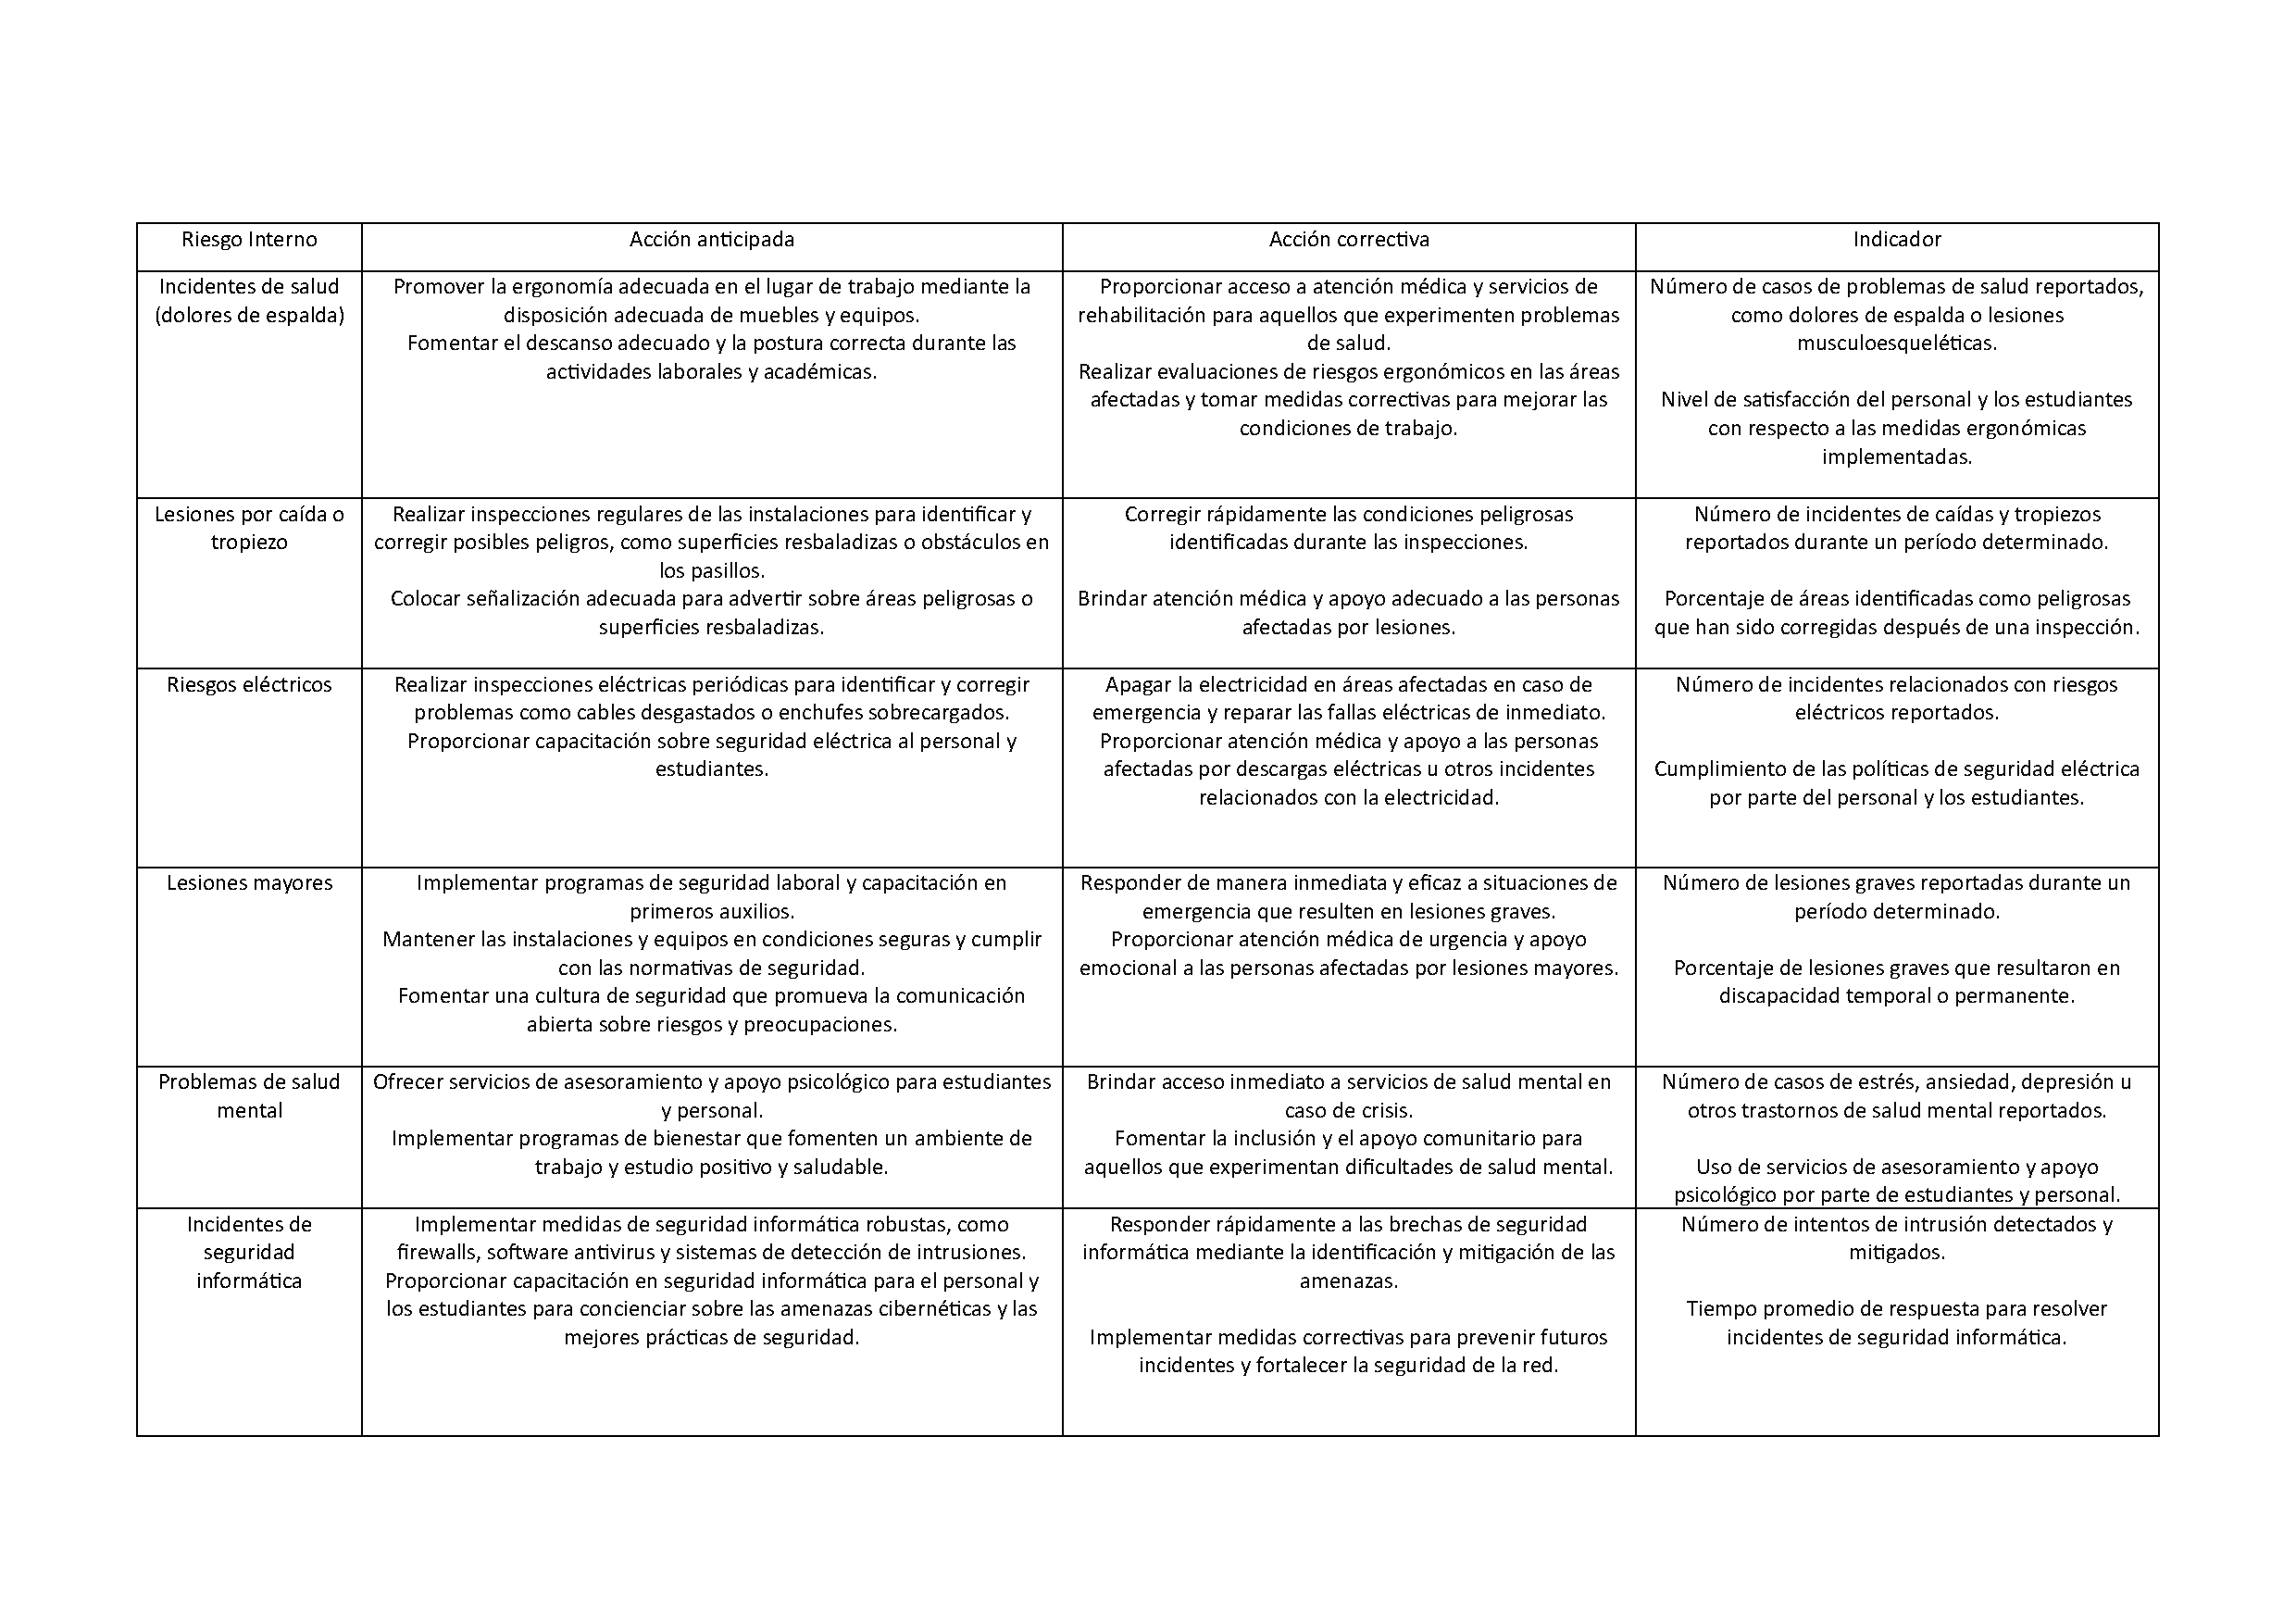
\includegraphics[scale=0.150]{21/img/accionesRiesgosInternos.pdf}
        \caption{Acciones para los riesgos Internos}
        \label{fig:accionesRiesgosInternos}
    \end{figure}
    
     
    \begin{figure}[H]
        \centering
        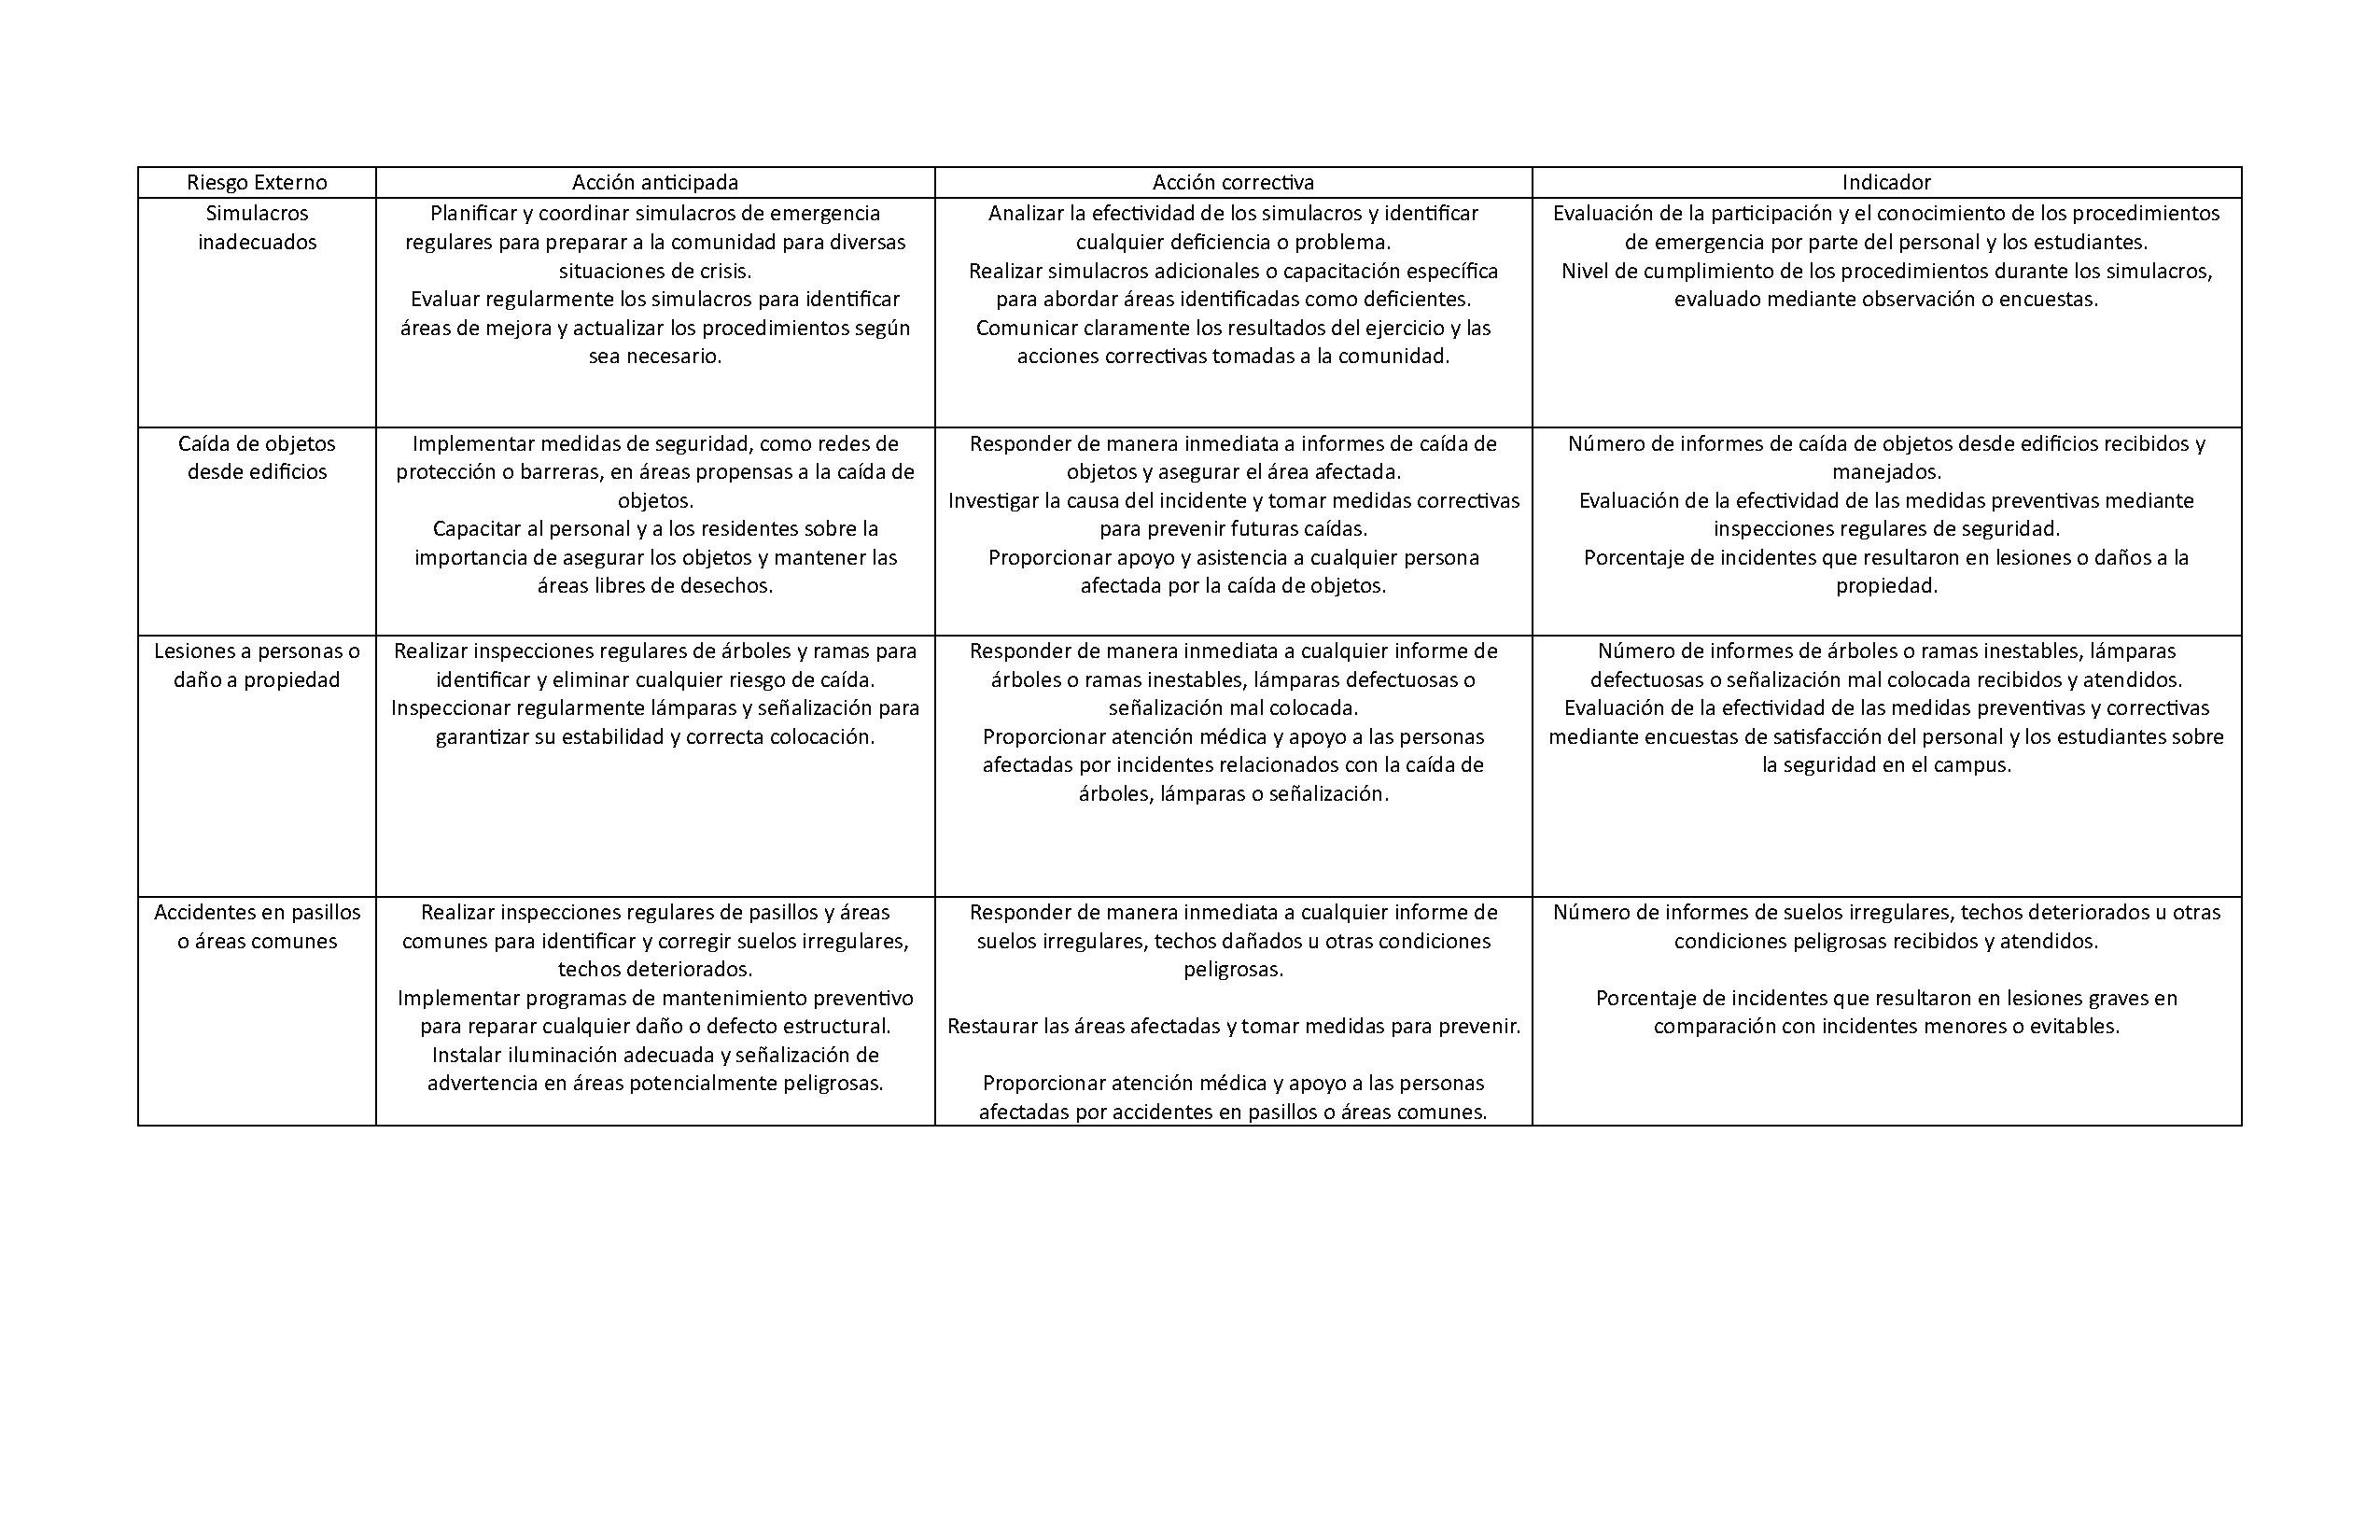
\includegraphics[scale=0.150]{21/img/accionesRiesgosExternos.pdf}
        \caption{Acciones para riesgos Externos.}
        \label{fig:accionesRiesgosExternos}
    \end{figure}
    
    % 
    % 
    
    % 
    \subsubsection{Identificación de capacidades}
    
    
    
    % 
    % 
    \subsubsection{Plano de localización de recursos}
    
    % 
    % 
    
    % 
    % 
    \subsubsection{ Identificación de apoyos externos}
    
    % Lugares que servir´andeapoyoenunsituaci´on
     %deemergencia.
    
    % 
    \subsubsection{Identificación de puntos de reunión}
    
    %\Zonaseguraencasodeunaevacuaci´ ondeemer
    %gencia.
    % 
    \subsubsection{Brigada de evacuación}
    
    %Acciones asignadas a cada integrante del equipo
     %de trabajo en caso de una evacuaci´ on de emer
    %gencia o repliegue.
    % 
    % 
    \subsubsection{Directorio de telefónicos de emergencia}
    
    Listado telefónico de instituciones de atención de emergencias y otras instituciones que intervengan para el seguimiento y control de las mismas las cuales se pueden observar en la siguiente Figura \ref{fig:directorioEmergencias}.
    
    \begin{figure}[H]
        \centering
        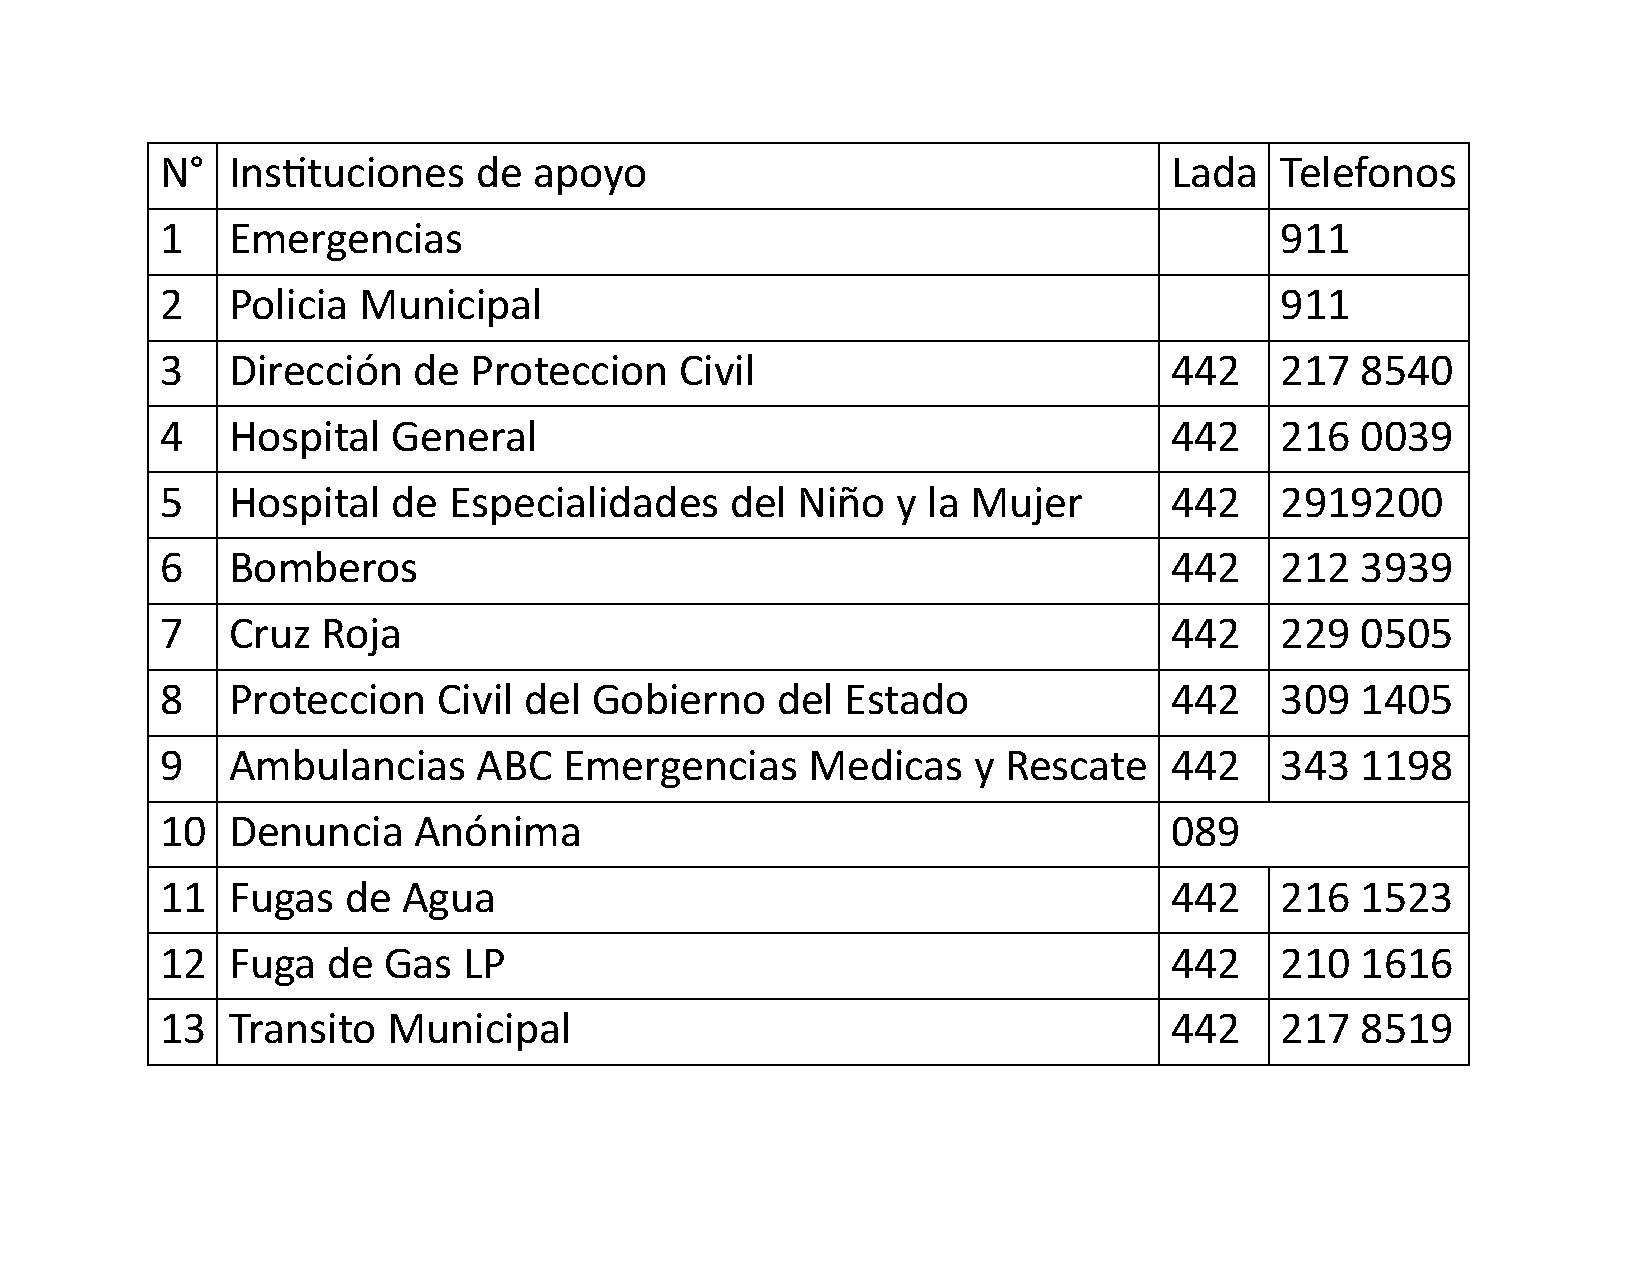
\includegraphics[scale=0.3]{21/img/directorioEmergecias.pdf}
        \caption{Directorio Telefónico de Emergencias.}
        \label{fig:directorioEmergencias}
    \end{figure}
    
    % 
    \subsection{Análisis de los métodos, materiales, herramientas e instalación utilizada en la ejecución del ensamble de un circuito electrónico}
    
    \subsubsection{Verificación}
    
    Costos de no calidad.
    % 
    % 
    \subsubsection{Desarrollo del sistema de tiempos predeterminado}
    \begin{figure}[H]
        \centering
        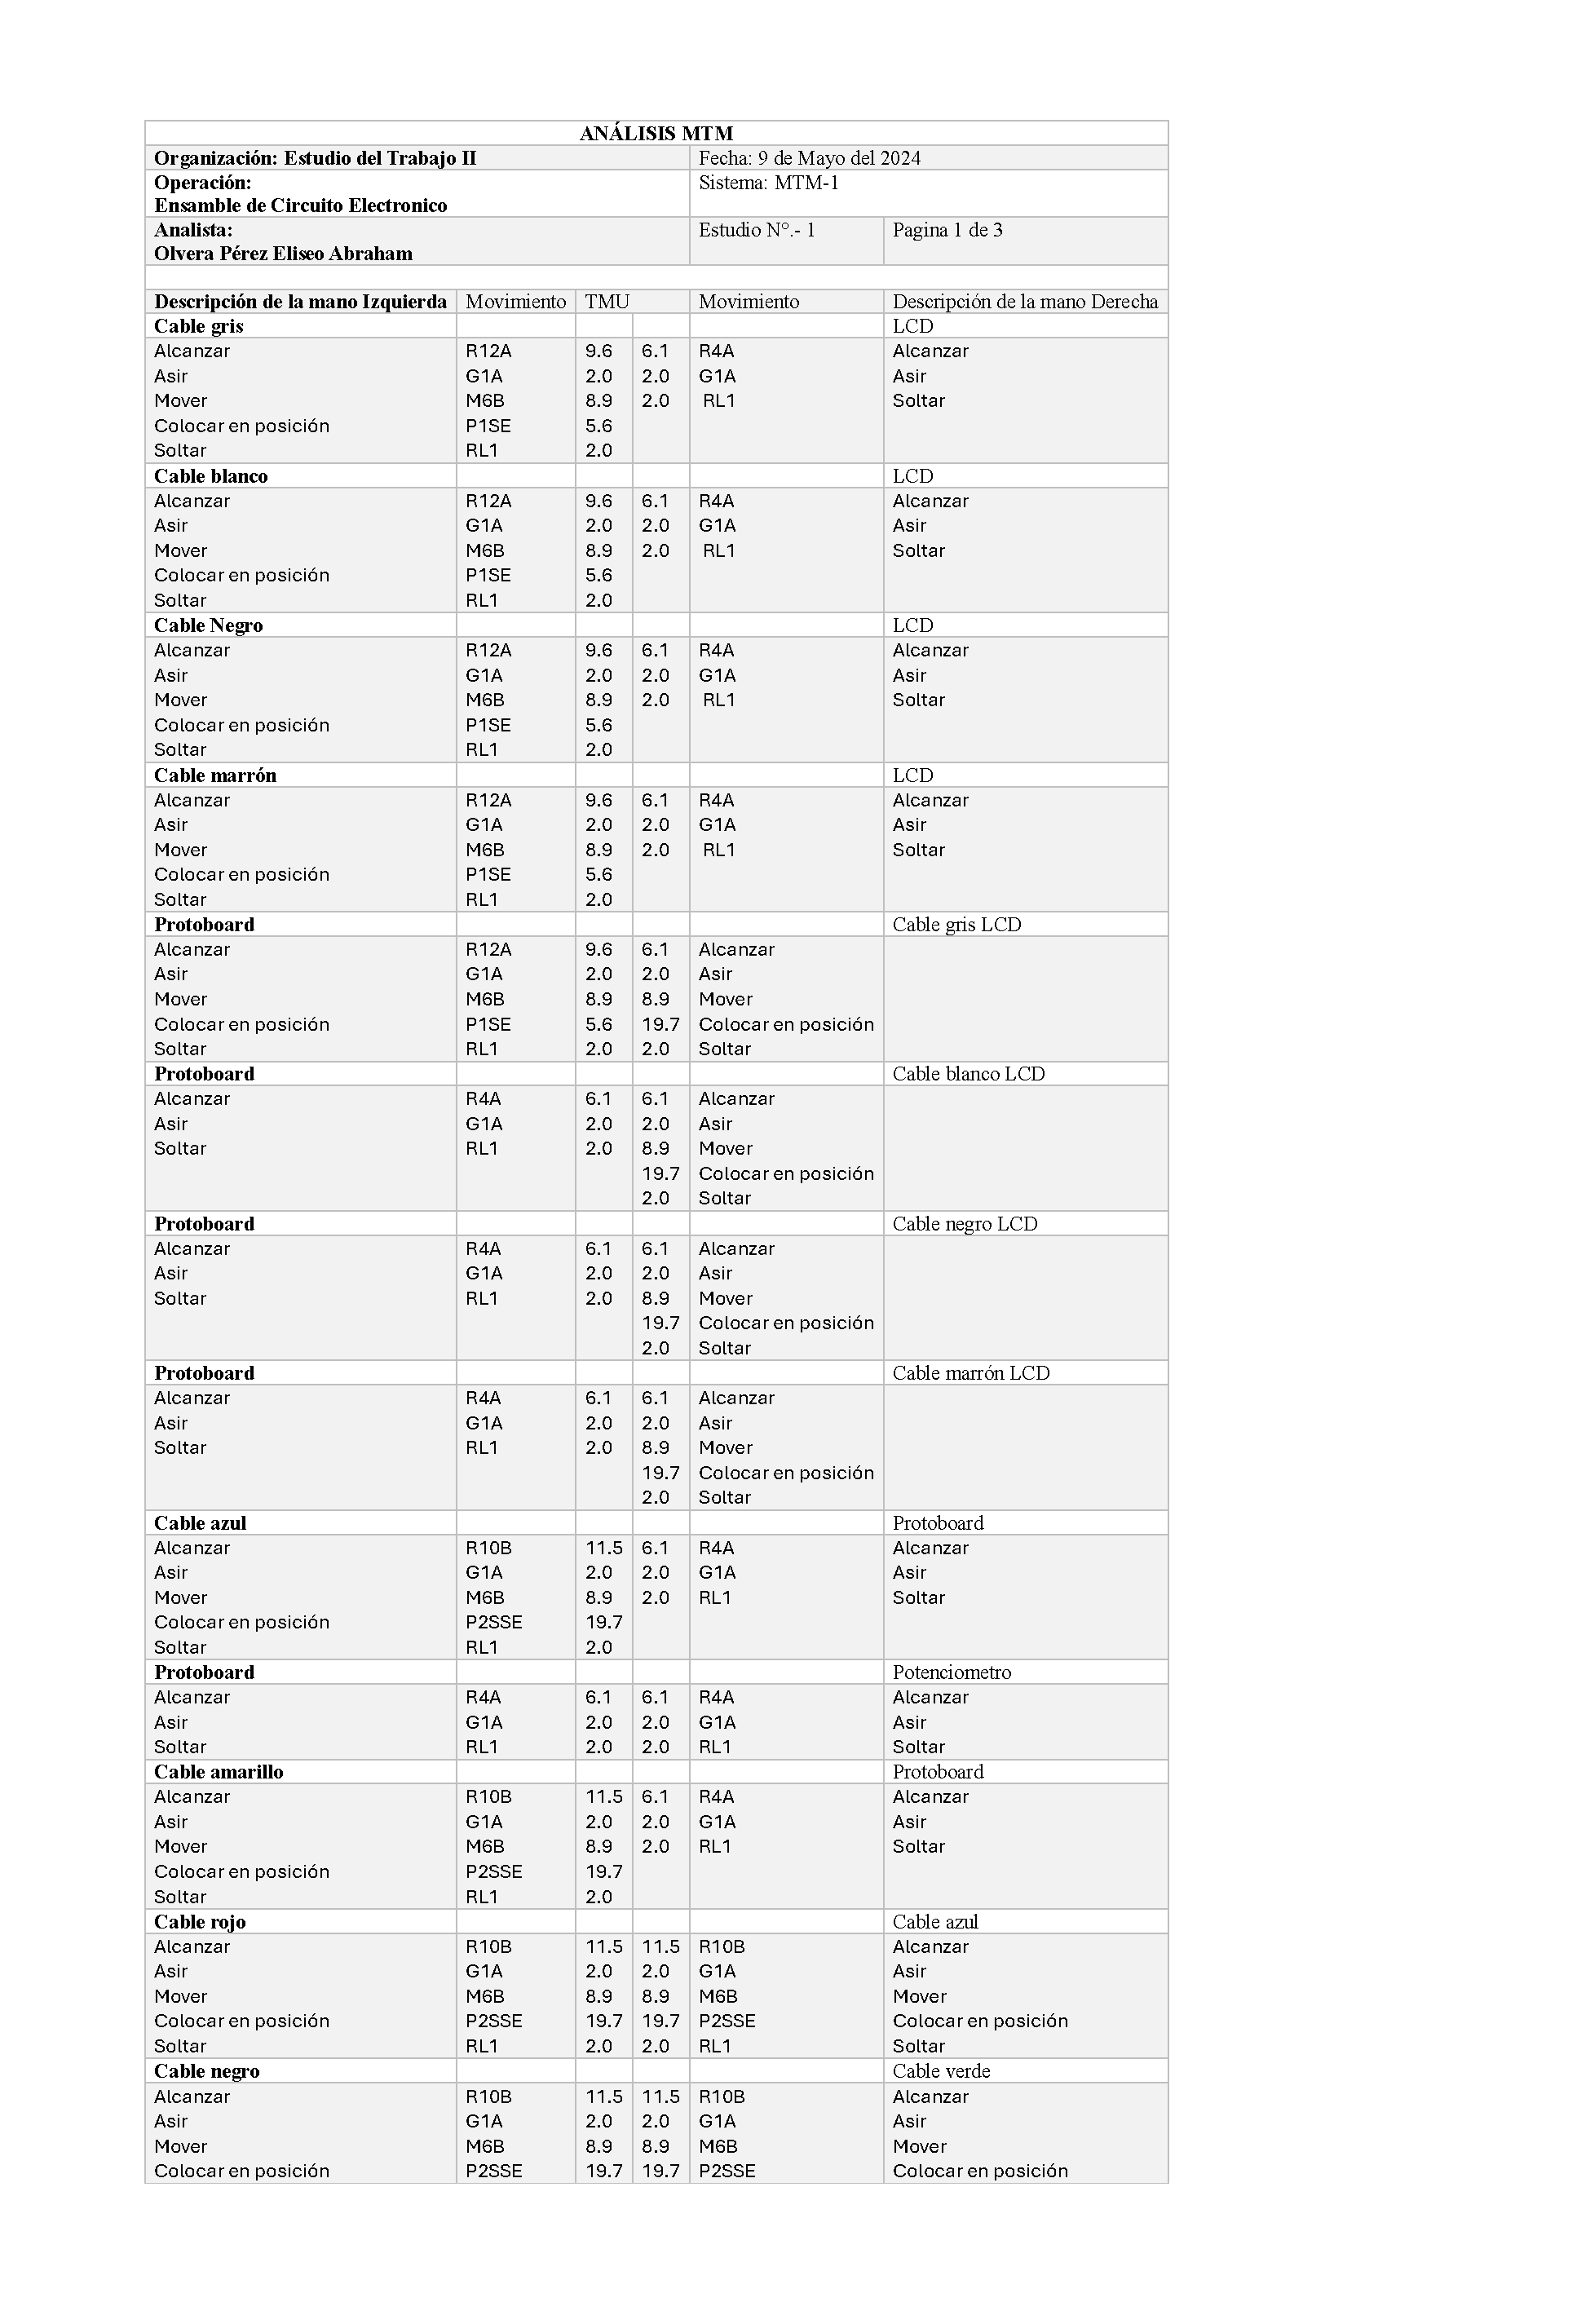
\includegraphics[scale=0.250]{21/img/analisisMTM.pdf}
        \caption{Sistema de tiempos predeterminados}
        \label{fig:analisisMTM}
    \end{figure}
    % 
    \subsubsection{Desarrollo del muestreo del trabajo}
    % 
    % 
    \subsubsection{Corrección por balanceo de procesos}
    % 
    % 
    \subsubsection{Datos estándar continuos y discretos}
    % 
    % 
    \subsection{Diseño de la forma más económica de realizar el trabajo}
    
    Una vez realizado la evaluación de materiales basado en su función e importancia para el ensamble, se pudo realizar una comparativa en la siguiente tabla, en la cual se muestra el conjunto de materiales que se usaron para realizar el "Ensamble defensor" y los nuevos materiales del "Ensamble retador".
    
    \begin{figure}[H]
        \centering
        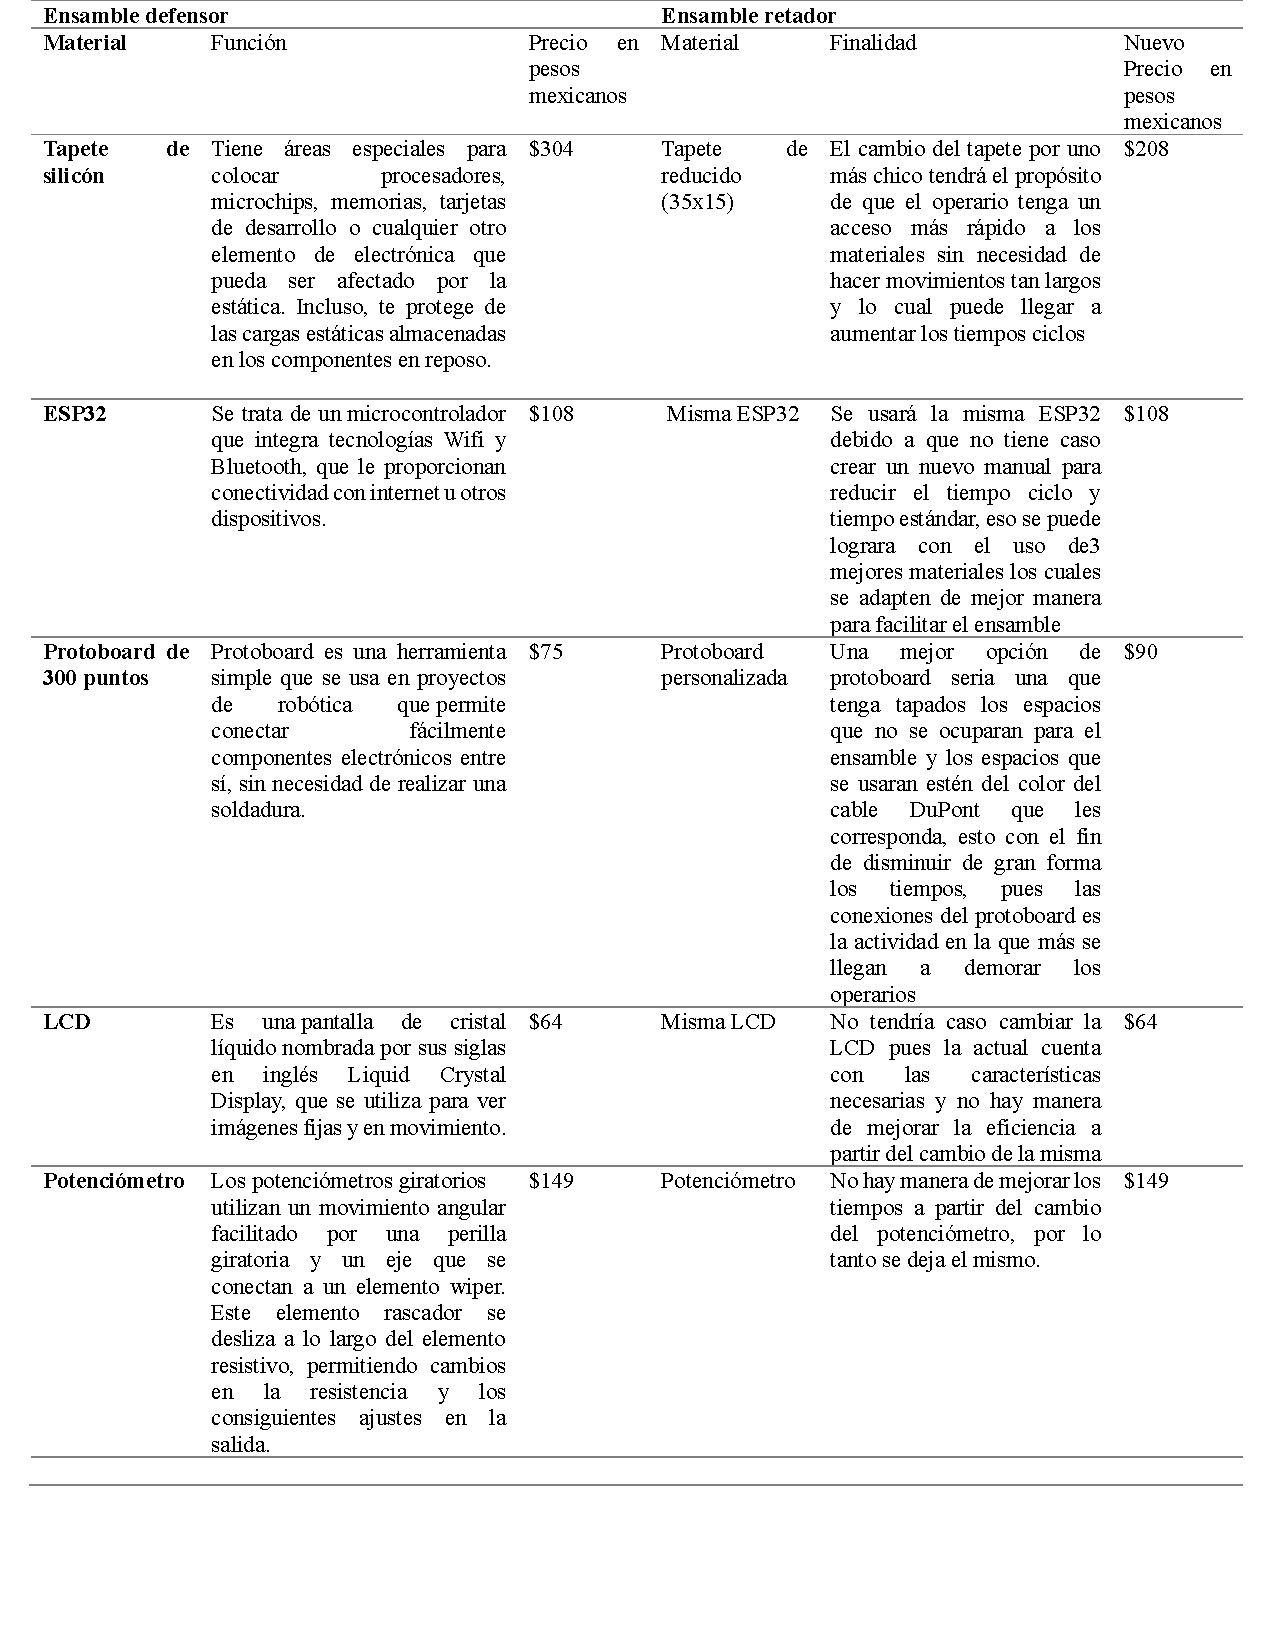
\includegraphics[scale=0.181]{21/img/comparacionPrecios.pdf}
        \caption{Tabla Comparatiba de precios de ensambles.}
        \label{fig:comparacionPrecios}
    \end{figure}
    
    Con esto podemos determinar que es mejor implementar el ensamble retador, ya que representa una disminución en el costo de los materiales.
    
    
    % 
    % 
    \subsection{Normalización de los métodos, materiales, herramientas e instalaciones}
    
    % 
    % 
    \subsection{Determinación del tiempo estándar para que una persona competente realice el trabajo con marcha normal}
    Los resultados del calculo del tiempo estándar para persona competente realice el trabajo con marcha normal de equipo y de los demás alumnos que forman parte de la clase de Estudio del Trabajo ll son:
    
    \begin{figure}[H]
        \centering
        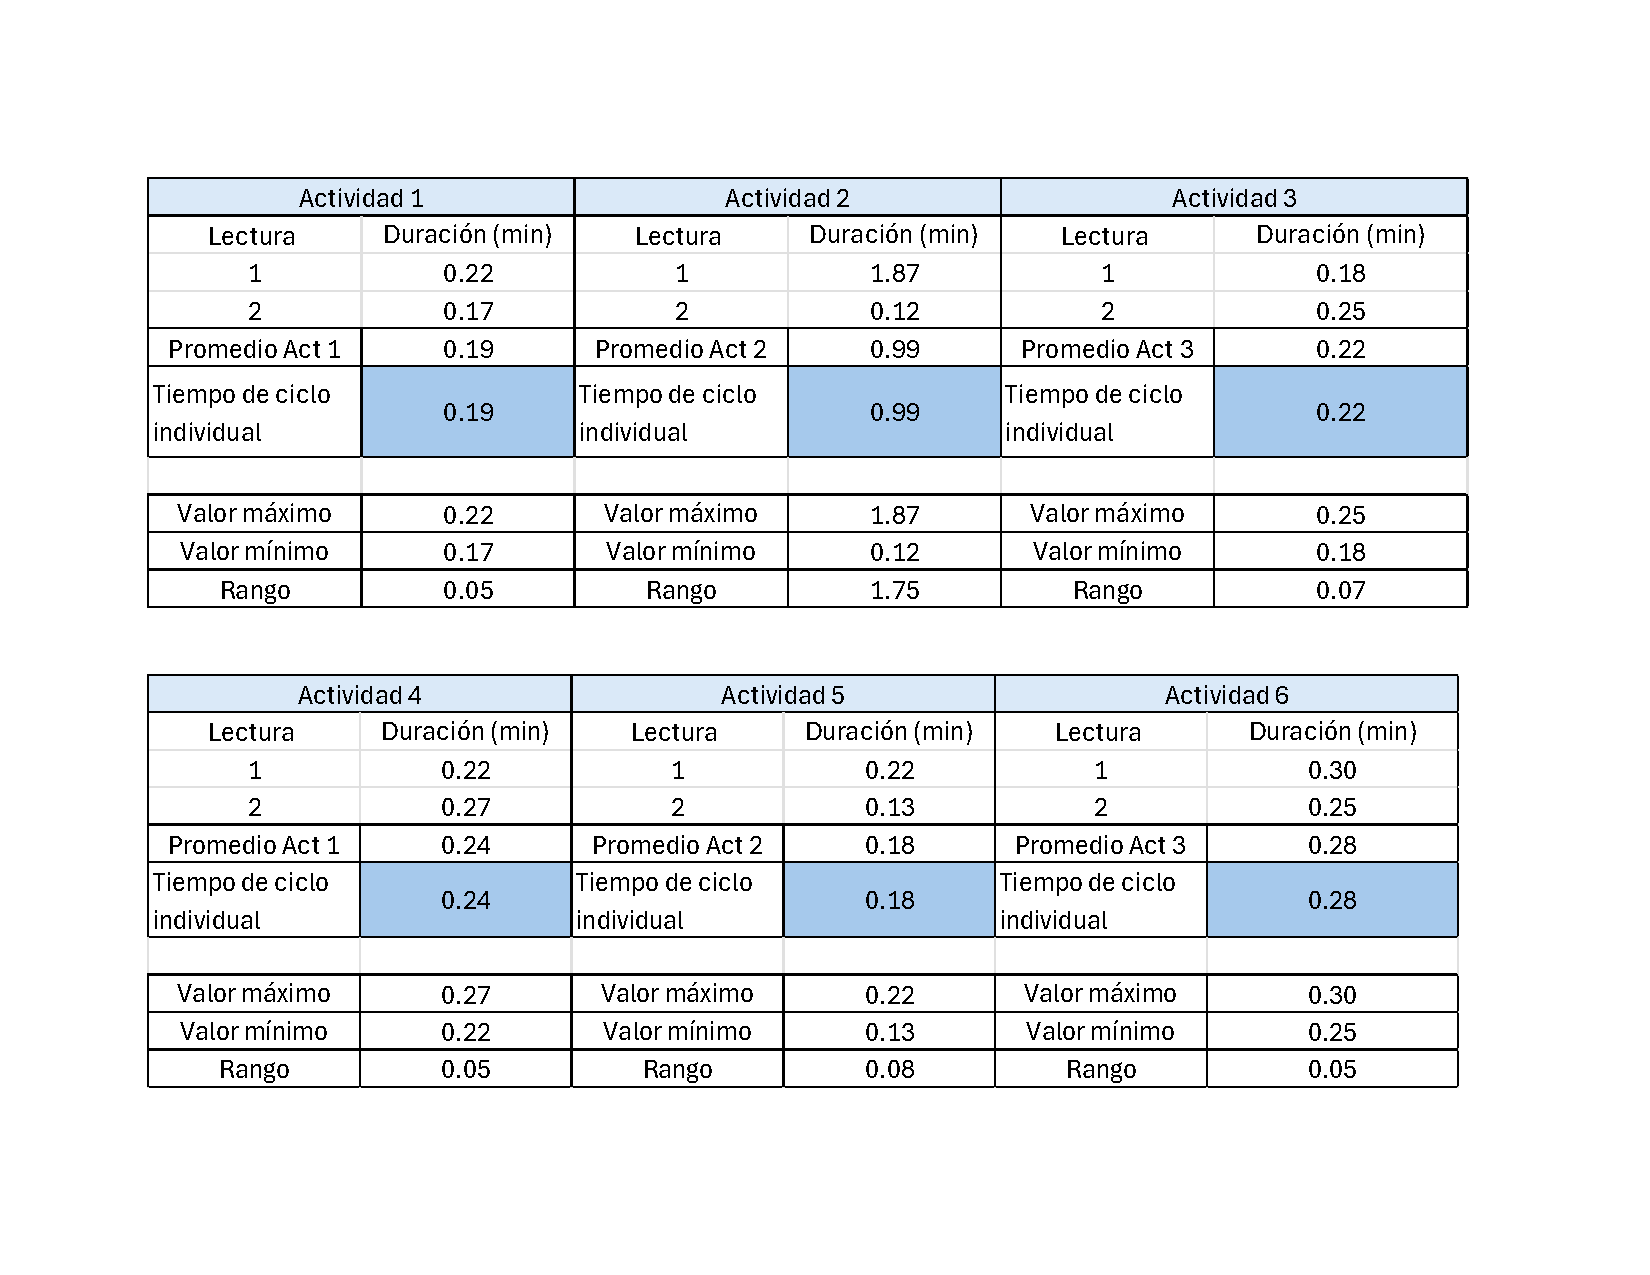
\includegraphics[scale=0.300]{21/img/tablasResultadosHolguras1.pdf}
        \caption{TablasResultadosHolguras1}
        \label{fig:tablasResultadosHolguras1}
    \end{figure}
    \begin{figure}[H]
        \centering
        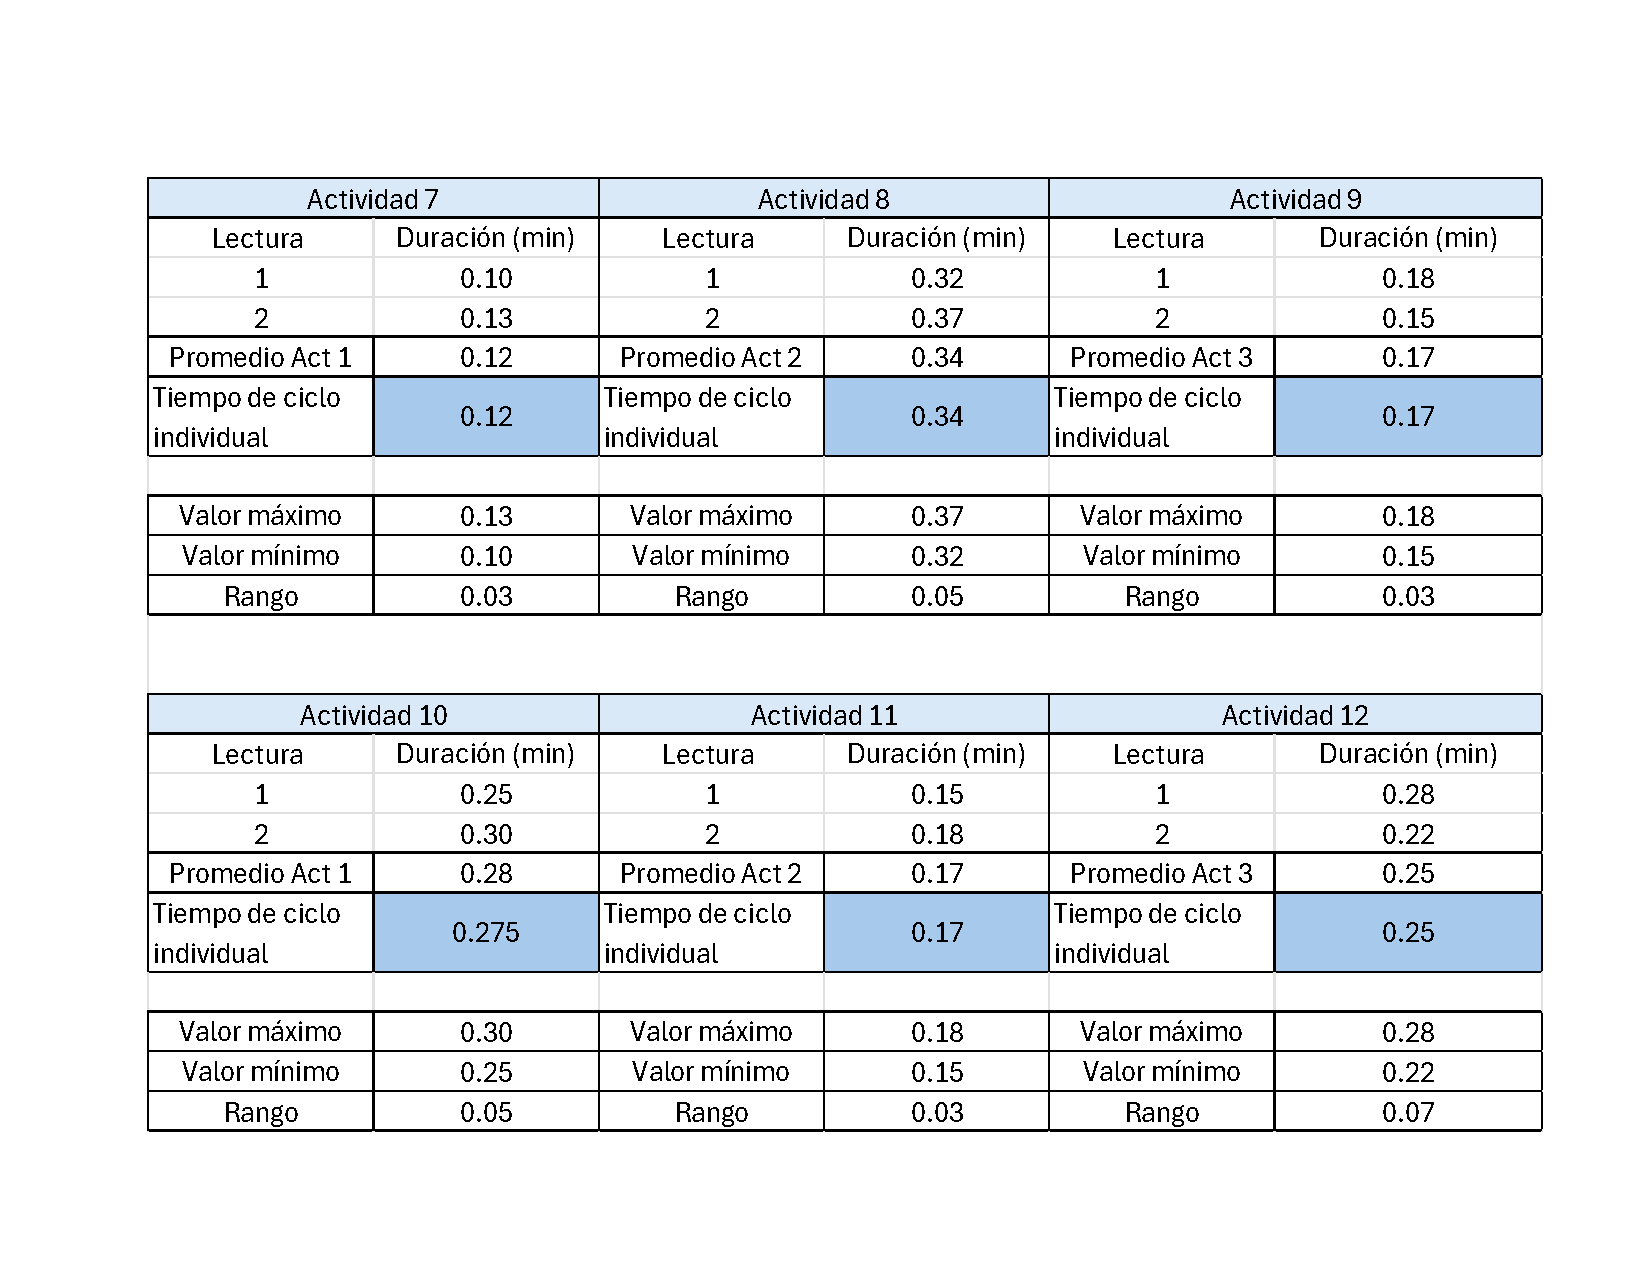
\includegraphics[scale=0.300]{21/img/tablasResultadosHolguras2.pdf}
        \caption{TablasResultadosHolguras2}
        \label{fig:tablasResultadosHolguras2}
    \end{figure}
    \begin{figure}[H]
        \centering
        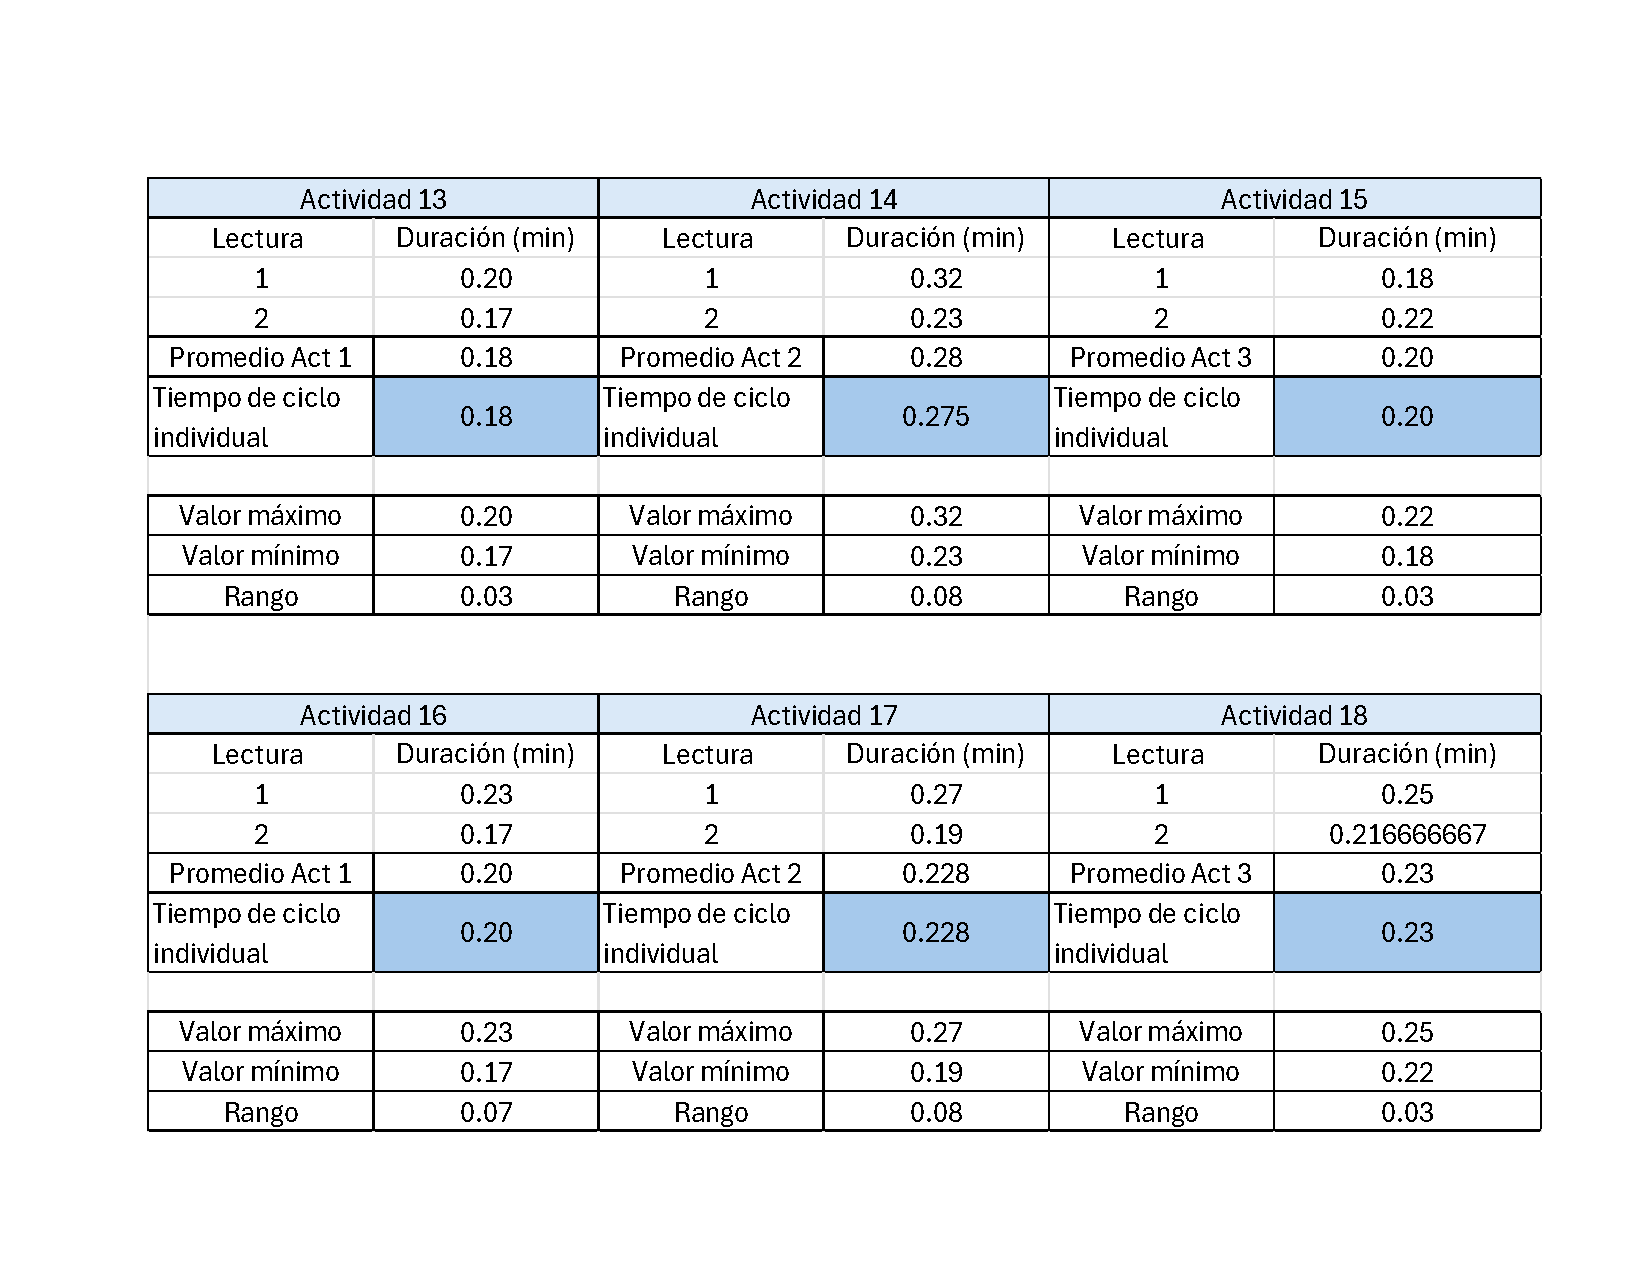
\includegraphics[scale=0.300]{21/img/tablasResultadosHolguras3.pdf}
        \caption{TablasResultadosHolguras3}
        \label{fig:tablasResultadosHolguras3}
    \end{figure}
    \begin{figure}[H]
        \centering
        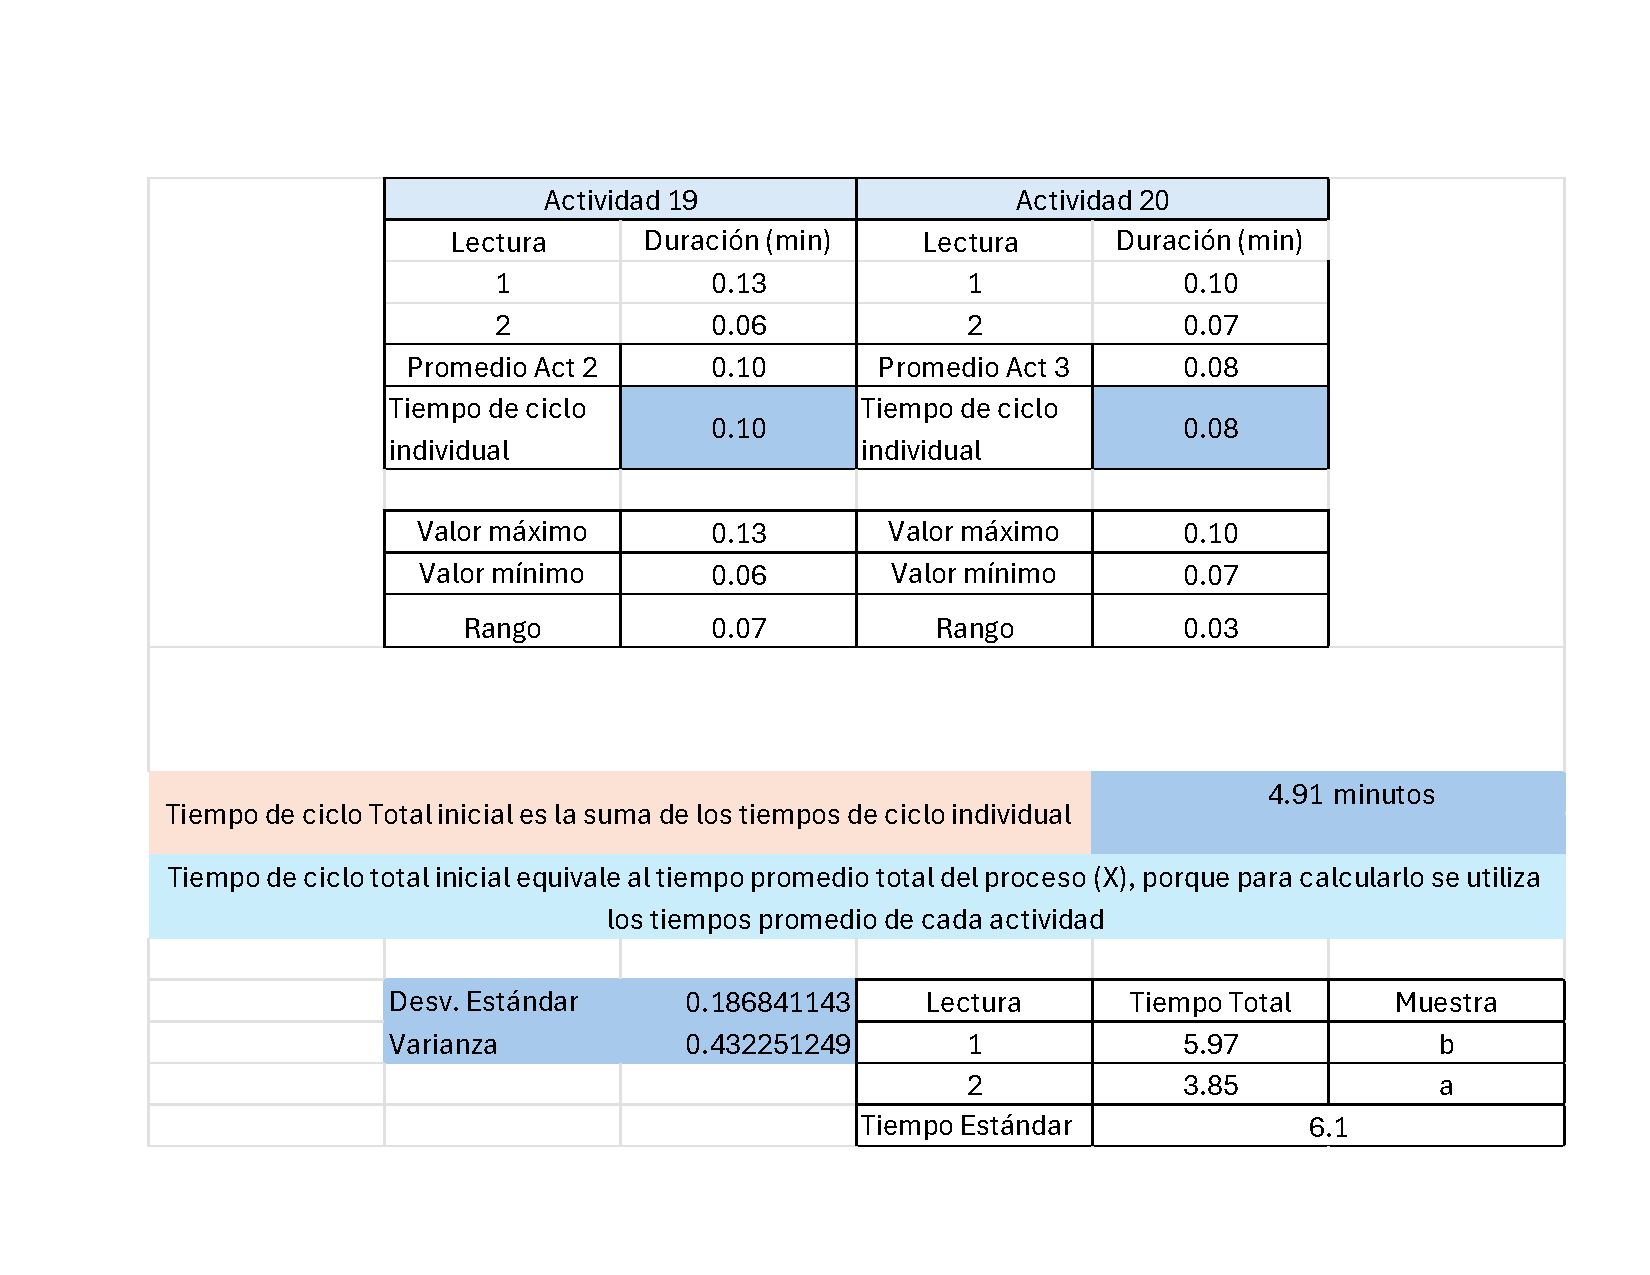
\includegraphics[scale=0.300]{21/img/tablasResultadosHolguras4.pdf}
        \caption{TablasResultadosHolguras4}
        \label{fig:tablasResultadosHolguras4}
    \end{figure}
    
    Y teniendo un tiempo estándar calculado de la siguiente manera: 
    
    \begin{figure}[H]
        \centering
        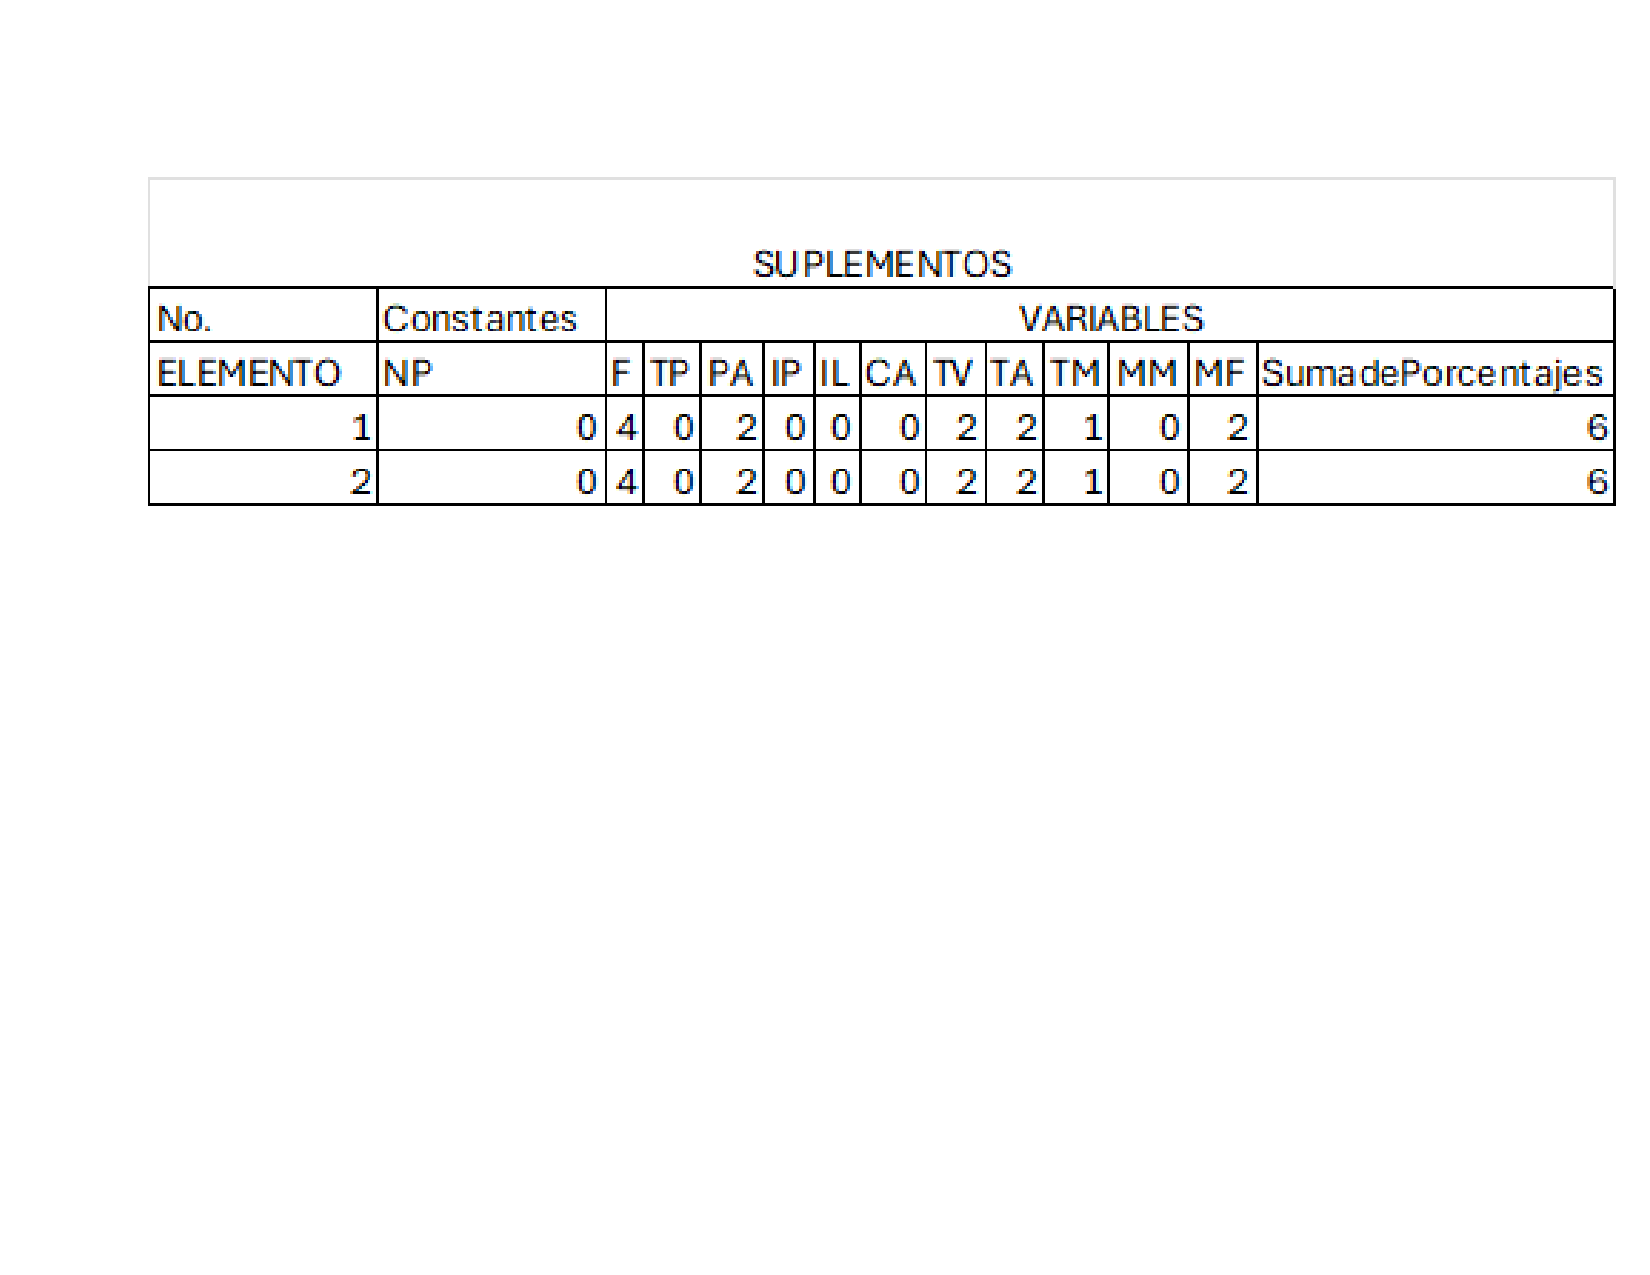
\includegraphics[scale=0.300]{21/img/suplementosResultados.pdf}
        \caption{TablasResultadosHolguras}
        \label{fig:suplementosResultados}
    \end{figure}
    
    \begin{figure}[H]
        \centering
        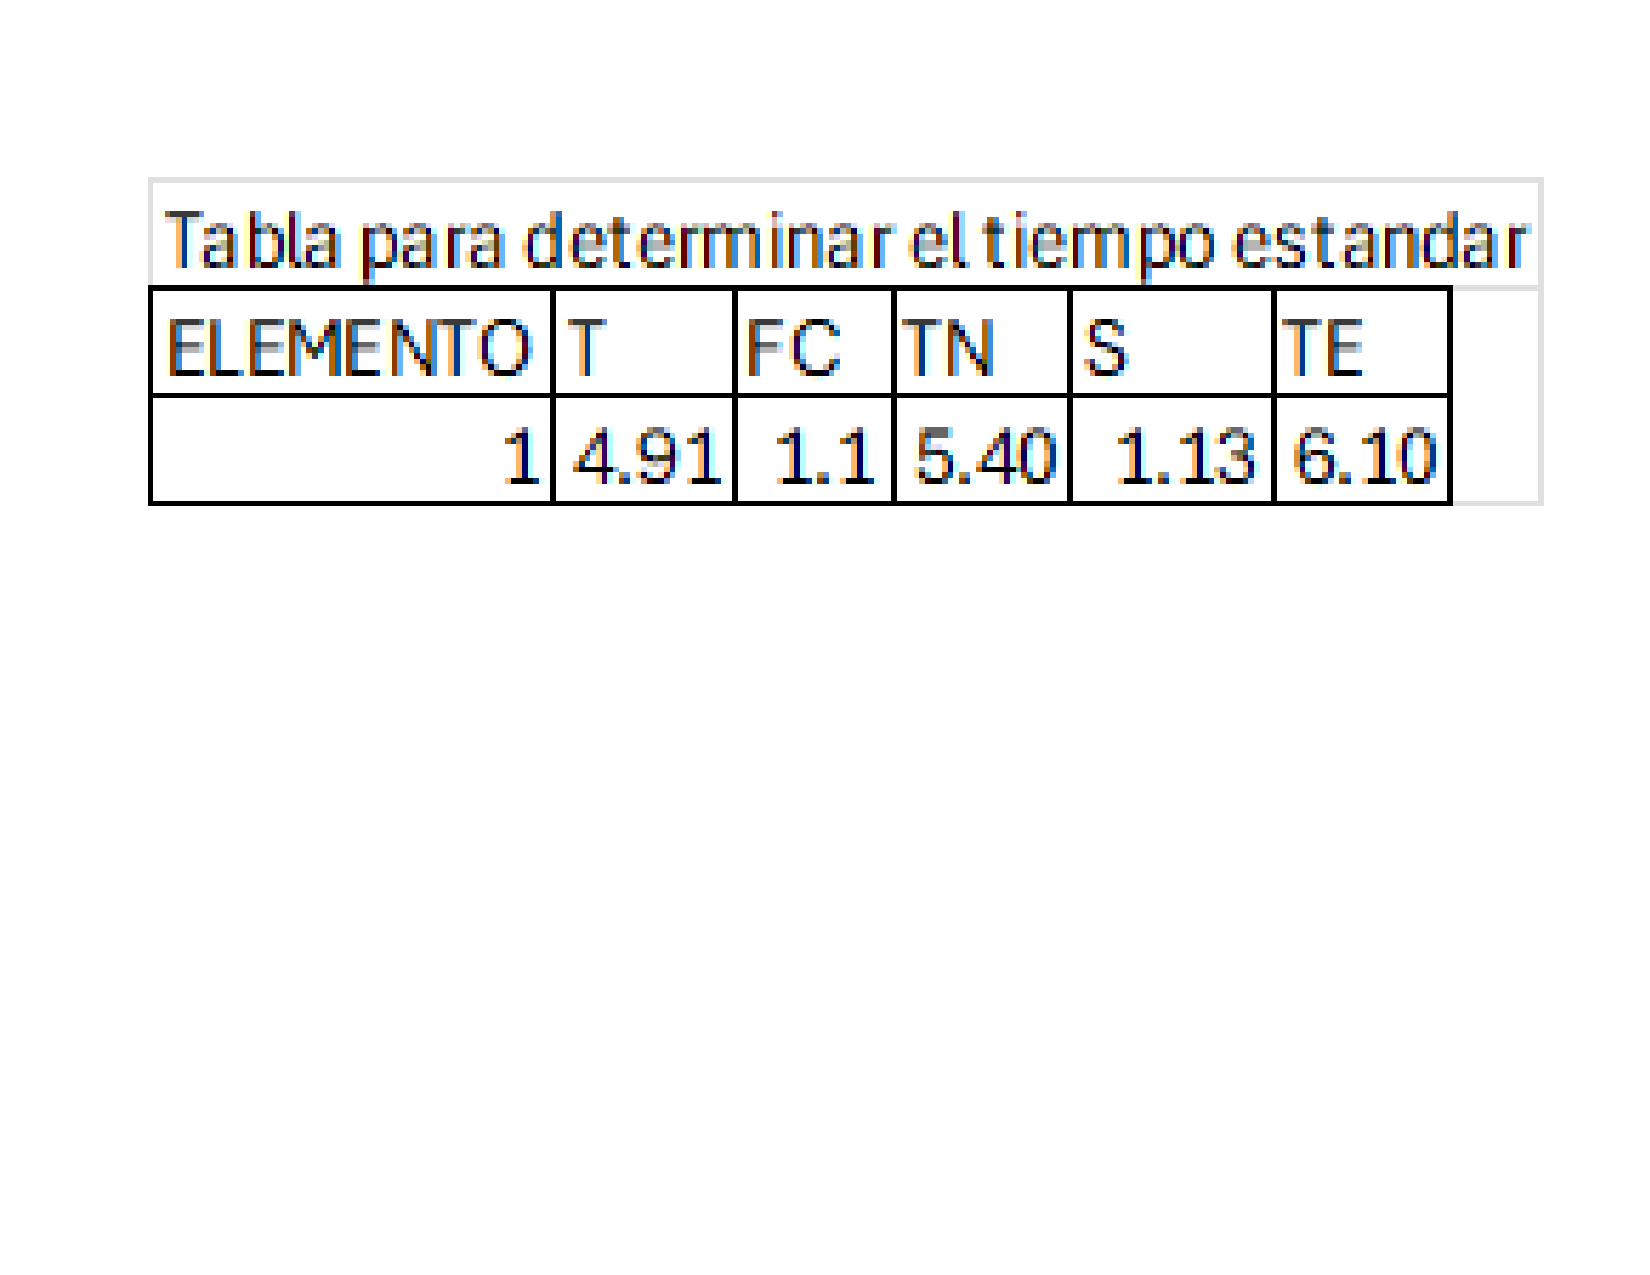
\includegraphics[scale=0.300]{21/img/suplementosResultados2.pdf}
        \caption{TablasResultadosHolguras}
        \label{fig:suplementosResultados2}
    \end{figure}
    
    De igual manera se realizo e calculo del tiempo estándar para 10 lecturas correspondientes a los demás alumnos, que son las siguientes: 
    \begin{figure}[H]
        \centering
        \includegraphics[scale=0.300]{21/img/tiempoEstandarCompañeros1.pdf}
        \caption{Tiempo Estándar en Conjunto}
        \label{fig:tiempoEstandarCompañeros1}
    \end{figure}
    
    \begin{figure}[H]
        \centering
        \includegraphics[scale=0.300]{21/img/tiempoEstandarCompañeros2.pdf}
        \caption{Tiempo Estándar en Conjunto}
        \label{fig:tiempoEstandarCompañeros2}
    \end{figure}
    \begin{figure}[H]
        \centering
        \includegraphics[scale=0.300]{21/img/tiempoEstandarCompañeros3.pdf}
        \caption{Tiempo Estándar en Conjunto}
        \label{fig:tiempoEstandarCompañeros3}
    \end{figure}
    %
    \begin{figure}[H]
        \centering
        \includegraphics[scale=0.300]{21/img/tiempoEstandarCompañeros4.pdf}
        \caption{Tiempo Estándar en Conjunto}
        \label{fig:tiempoEstandarCompañeros4}
    \end{figure}
    \begin{figure}[H]
        \centering
        \includegraphics[scale=0.300]{21/img/tiempoEstandarCompañeros5.pdf}
        \caption{Tiempo Estándar en Conjunto}
        \label{fig:tiempoEstandarCompañeros5}
    \end{figure}
    
    \begin{figure}[H]
        \centering
        \includegraphics[scale=0.300]{21/img/tiempoEstandarCompañeros6.pdf}
        \caption{Tiempo Estándar en Conjunto}
        \label{fig:tiempoEstandarCompañeros6}
    \end{figure}
    
    
    
    \section{Conclusiones}
    
    El objetivo de este trabajo fue desarrollar un proyecto integrador basado en el ensamblaje de un circuito. Para su realización, fue necesario aplicar todos los conocimientos adquiridos a lo largo del semestre, incluyendo el estudio de movimientos y tiempos, así como muestras continuas y discretas. Este proyecto no solo requería el dominio de los conceptos de estudio del trabajo II, sino que también se complementaba con conocimientos de otras materias, tales como probabilidad y estadística, higiene y salud, y estudio del trabajo I.
    
    Nuestro principal objetivo era diseñar, mejorar e integrar sistemas productivos de bienes y servicios, aplicando tecnologías para su optimización y determinando el tiempo estándar en el ensamblaje del circuito. No obstante, el proyecto integrador no pudo completarse debido a complicaciones surgidas durante el semestre, como retrasos relacionados con la ESP32 y otros factores. Sin embargo, el trabajo realizado no fue en vano, ya que aprendimos mucho sobre la normalización de procesos a nivel profesional y cómo los conocimientos de distintas materias se complementan en proyectos específicos.
    
    Diseñamos un ensamblaje electrónico y creamos un manual para capacitar a operarios sin experiencia en este tipo de ensamblajes. Realizamos dos pruebas de ensamblaje y desarrollamos un análisis para identificar oportunidades de optimización y cambios en los materiales utilizados, con el fin de reducir costos y aumentar la eficiencia del ensamblaje, facilitando así el trabajo del operario. También utilizamos herramientas como Overleaf, GitHub y Visual Studio, que son comunes en la industria, adquiriendo un conocimiento preliminar sobre su uso.
    
    A través de estos pasos y la aplicación conjunta de metodologías, herramientas y conocimientos, logramos determinar un tiempo estándar a partir de los tiempos de ciclo de las diferentes actividades del ensamblaje. No solo obtuvimos un tiempo estándar individual, sino que también conseguimos un tiempo estándar colectivo gracias a las distintas mediciones de tiempos de diversos operarios.
    
    Aunque el proyecto integrador no se completó en su totalidad, se alcanzaron la mayoría de los objetivos y se corroboró la hipótesis casi en su totalidad. Este trabajo nos permitió vislumbrar los desafíos que enfrentaremos como futuros ingenieros industriales y nos proporcionó aprendizajes valiosos que serán de gran utilidad, superando el simple hecho de aprobar una materia.
    
    \section{Agradecimientos}
    
    Es importante darles su debido reconocimiento a los laboratorios, instituciones, organizaciones, entre otros que han sido participes para la culminación de este trabajo. También es importante mencionar, fondos, proyectos, becas, entre otros que se le han otorgado al o los autores para realizar el trabajo de investigación. Ejemplo: “Los autores agradecen al Concejo Nacional de Ciencia y Tecnología por los recursos otorgados…”
    
    % \section*{Referencias}
    
    % Para esta platilla, se solicita al autor enumerar las citas de manera consecutiva entre corchetes \cite{YLi2013}. 
    % La puntuación de la oración que sigues sería \cite{Mesaelides2011}. 
    % Refiérase simplemente al número de referencia, como en \cite{Morales2012}, no utilice “Ref. [3]” o “referencia [3]” excepto al principio de una oración: “La referencia [3] fue la primera…”
    % Enumere las notas al pie por separado en superíndices. Coloque la nota de pie de en la parte inferior de la columna en la que se citó. No coloque notas al pie en la lista de referencias. Utilice letras para las notas al pie de la tabla.
    % A menos de que haya tres autores o más; no utilice “et al.”. Los trabajos que no hayan sido publicados, incluso si han sido presentados para su publicación, deben ser citados como “inéditos”. Los trabajos que han sido aceptados para su publicación deben de citarse como “en prensa”. Poner en mayúscula sólo la primera palabra de un título, excepto los nombres propios y los símbolos de elemento. 
    % Otros ejemplos \cite{LAAngeles2021}, \cite{LAAngelesConni}. 
    % Véase el link \cite{prueba}, Véase el Apéndice \ref{anexo:pines}.
    
    % Ejemplo
    %  @Article{article,
    % 	author = "Author1 LastName1 and Author2 LastName2 and Author3 LastName3",
    % 	title = "Article Title",
    % 	volume = "30",
    % 	number = "30",
    % 	pages = "10127-10134",
    % 	year = "2013",
    % 	doi = "10.3389/fnins.2013.12345",
    % 	URL = "http://www.frontiersin.org/Journal/10.3389/fnins.2013.12345/abstract",
    % 	journal = "Frontiers in Neuroscience"
    % }
    
    % @book{book,
    %   author    = {Author Name}, 
    %   title     = {The title of the work},
    %   publisher = {The name of the publisher},
    %   address   = {The city},
    %   year      = 1993,
    % }
    
    % @incollection{chapter,
    %   author       = {Bauthor Surname}, 
    %   title        = {The title of the work},
    %   editor       = {Editor Name},
    %   booktitle    = {The title of the book},
    %   publisher    = {The name of the publisher},
    %   address      = {The city},
    %   year         = 2002,
    %   pages        = {201-213},
    % }
    
    % @InProceedings{conference,
    %   author = {Cauthor Name and Dauthor Surname and Fauthor LastName},
    %   title = {The title of the work},
    %   booktitle = {The title of the conference proceedings},
    %   year = 1996,
    %   publisher = {The name of the publisher},
    %   editor = {Editor Name1 and Editor Name2},
    %   pages = {41-50},
    % }
    
    % @book{cho,
    %   author       = {Gauthor Name1}, 
    %   title        = {The title of the work},
    %   publisher = {Country code and patent number},
    %   address      = {Patent Country},
    %   year = 2013
    % }
    
    % @book{patent,
    %   author    = {Hauthor Surname1}, 
    %   title     = {The title of the work},
    %   publisher = {Patent number},
    %   address   = {Patent country},
    %   year      = 2010,
    % }
    
    % % please use misc for datasets
    % @misc{dataset, 
    % 	author = "Author1 LastName1 and Author2 LastName2 and Author3 LastName3",
    % 	title = "Data Title",
    % 	year = "2011",
    % 	doi = "10.000/55555",
    % 	URL = "http://www.frontiersin.org/",
    % }
    
    \bibliographystyle{ieeetr}
    \bibliography{21/referencias}
    % 
    % 
    %%%%%%%%%%%%%%%%%%%%%%%%%%%%%%%%%%
    \appendix
    %%%%%%%%%%%%%%%%%%%%%%%%%%%%%%%%%%
    % 
    % 
    % \centering{\section[\appendixautorefname{}]{Apéndice}}\label{anexo:pines}
    % \includepdf[pages=-]{6/Img/pines.pdf}
    %%%%%%%%%%%%%%%%%%%%%%%%%%%%%%%%%%%%%%%%